\documentclass[11pt]{report}
\usepackage[a4paper, margin=1in]{geometry}
\usepackage{setspace}
\usepackage{graphicx}
\usepackage{amsmath}
\usepackage{amssymb}
\usepackage{float}
\usepackage{caption}
\usepackage{svg}
\usepackage{braket}


\usepackage{tikz}
\usetikzlibrary{matrix, arrows.meta, positioning, calc}


\usepackage{subcaption}


\usepackage{xcolor}
\definecolor{ethblue}{HTML}{215CAF}
\definecolor{ethpetrol}{HTML}{00596D}
\definecolor{ethgrey}{HTML}{575757}



\usepackage{hyperref}
\hypersetup{
    colorlinks=true,
    linkcolor=ethpetrol,
    citecolor=ethpetrol,
    urlcolor=ethpetrol
    }



\usepackage{titlesec}
\titleformat{\chapter}[display]
  {\normalfont\huge\bfseries}
  {\color{ethgrey}\chaptertitlename\ \thechapter}
  {20pt}
  {\Huge}

\titleformat{\section}
  {\normalfont\Large\bfseries}
  {\color{ethgrey}\thesection}
  {1em}{}

\titleformat{\subsection}
  {\normalfont\large\bfseries}
  {\color{ethgrey}\thesubsection}
  {1em}{}

\titleformat{\subsubsection}
  {\normalfont\normalsize\bfseries}
  {\thesubsubsection}
  {1em}{}



\usepackage{fancyhdr}
\pagestyle{fancy}
\fancyhf{}

\fancyhead[L]{\color{ethgrey}\nouppercase{\leftmark}}
\fancyfoot[C]{\color{ethgrey}\thepage}

\renewcommand{\headrulewidth}{0.4pt}
\renewcommand{\headrule}{\color{ethgrey}\hrule width\headwidth height\headrulewidth}
\renewcommand{\footrulewidth}{0pt}

\renewcommand{\chaptermark}[1]{\markboth{\thechapter.\ #1}{}}



\usepackage[style=numeric-comp,citetracker=true]{biblatex}
\addbibresource{bibliography.bib}
\setlength{\bibitemsep}{1.2\itemsep}
%\AtEveryBibitem{%
%  \ifciteseen
%    {}
%    {\color{red}}
%}


\AtEveryBibitem{%
  \ifboolexpr{ test {\iffieldundef{doi}} }
    {}
    {\clearfield{url}}% doi present -> drop url
}

\AtEveryBibitem{\clearfield{isbn}\clearfield{issn}\clearfield{month}}




\newcommand{\checkthis}[1]{{\color{red}\bfseries [ #1 ]}}
\newcommand{\question}[1]{{\color{green}\bfseries [??? #1 ???]}}

\begin{document}


    \begin{titlepage}

        
\includegraphics[width=0.4\textwidth]{plots/eth-logo-pos.png}\par
        \centering 
        \vspace*{4cm}
        {\LARGE \bfseries Fractional Topological Phases in Two-Dimensional Moir\'e Systems \par}
        \vspace{1.5cm}
        {\Large Bartłomiej Leks \par}
        \vspace{0.5cm}
        {\large Master's Thesis \par}
        \vspace{0.3cm}
        {\large Department of Materials Science, ETH Zurich \par}
        \vspace{1cm}
        {\large \textbf{Supervisors:} \par Dr.\ Glenn Wagner \par Prof.\ Peter Derlet}
        \vfill
        {\large \today \par}
    \end{titlepage}

    \begin{abstract}
      abstract
    \end{abstract}
    \tableofcontents
    \newpage

    \chapter{Introduction}\label{ch:introduction}
        \section{Moir\'e materials \& Transition metal dichalcogenides}
    
    Moir\'e materials are two-dimensional heterostructures formed by stacking atomically thin materials, with a small lattice mismatch or a twist angle between them. Due to this misalignment, a spatial interference pattern is formed between the two lattices, which leads to a formation of an artificial crystal with a substantially larger lattice constant --- Moir\'e lattice. In small angle approximation the moire lattice constant is $a_m \approx \frac{a_0}{\theta}$, leading to an increase of the lattice constant by an order of magnitude for typical twist angles of $\theta \in (0, 4^\circ)$.
This in turn leads to effective folding of the Brillouin zone (BZ) of the original material and emergence of Moir\'e bands in the band structure. The separation of length scales between the Moir\'e lattice and the original lattice and the Moir\'e unit cell, leads to a significant enhancement of the effects of interaction relative to the kinetic energy, leading to a plethora of strongly correlated phases of matter.

    Owing to this trait and the unique wide tunability the properties, the field of Moir\'e materials has sparked a revolution in modern condensed matter physics.
    Specifically, the properties can be tuned through:
    \begin{itemize}
        \item A wide choice of constituent 2D materials: graphene, transition metal dichalcogenides (TMDs), transition metal oxides~\cite{li2025twist} and their combinations into multilayer structures
        \item Control over the twist angle between the layers --- changing the Moir\'e lattice constant $a_m$, hybridization between the layers, and in effect the band structure
        \item Strain engineering~\cite{escudero2024designing}
        \item Screening of Coulomb interactions through dielectric environment engineering~\cite{zhao2023probing}
        \item Continuous \textit{in situ} control over the filling of unit cells--- controlling the electron filling of each Moir\'e unit cell
    \end{itemize}

    \begin{figure}[htbp]
        \centering
        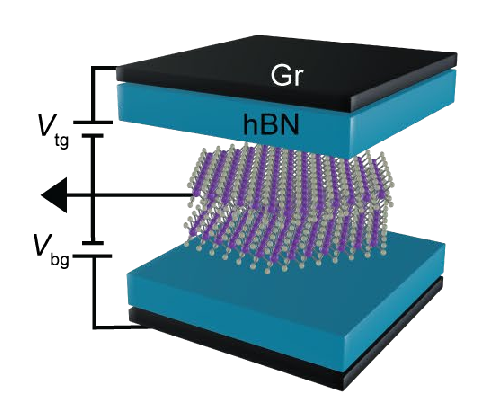
\includegraphics[width=0.5\textwidth]{plots/experimental_setup.png}
        \caption{Experimental setup of a Moir\'e material sandwiched between two spacers and two conducting gates, adapted from~\cite{Cai2023}.}\label{fig:experimental_setup}
    \end{figure}

    The last two points can be easily understood when one considers a typical experimental setup (Fig.~\ref{fig:experimental_setup}), where the material is sandwiched between two spacers and two conducting gates~\cite{Cai2023}. First, the dielectric properties of the spacer, and the distance of the gates from the sample directly affect the screening of electron-electron interactions within the active material. Second, when the gate potential is tuned, due the large periodicity of the material, the electron filling of each Moir\'e unit cell can be easily controlled --- enabling doping by an order of 10 electrons per unit cell.

    \subsection{Transition metal dichalcogenides}
    While the emergence of Moir\'e materials as a prolific research field was catalyzed by the discovery of superconductivity and correlated insulators in twisted bilayer graphene (TBG)~\cite{cao2018correlated, cao2018unconventional}, semiconductor materials joined the field soon after~\cite{mak2022semiconductor}. One of the important features of Moir\'e materials is the emergence of flat bands caused by the large lattice constant of Moir\'e lattice and folding of the brillouin zone --- effective confinement of electrons and suppression of the kinetic energy. However, in heterostructures made from graphene --- described by massless Dirac fermions~\cite{novoselov2005two} (no energy gap) --- the flat bands emerge only at special ``magic'' angles. On the other hand, in semiconductors due to their non-zero bandgap, the condition is relaxed~\cite{wu2018hubbard}. While magic angles can still be identified~\cite{devakul2021magic}, the material is gapped over a wide range of angles and the angle can be continuously tuned. In this class of materials, homobilayers of transition metal dichalcogenides (TMDs) are of particular interest due to
    \begin{itemize}
        \item Relatively simple structure (two layers of the same material)
        \item Relatively low disorder densities
        \item Direct bandgap
        \item Spin-valley locking~\cite{mak2022semiconductor}
    \end{itemize}

    \begin{figure}[htbp]
        \centering
        \begin{subfigure}[b]{0.1\textwidth}
            \centering
            
            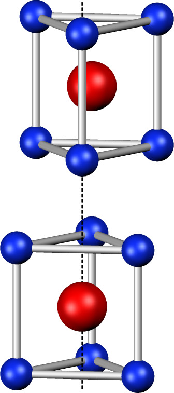
\includegraphics[width=1.0\textwidth]{plots/tmd1.png}
            \subcaption{}\label{fig:tmd_struct1}
        \end{subfigure}
        \hfill
        \begin{subfigure}[b]{0.3\textwidth}
            \centering
            
            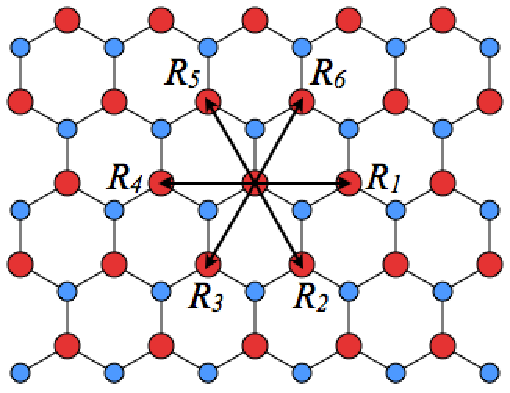
\includegraphics[width=1.0\textwidth]{plots/image8.png}
            \subcaption{}\label{fig:tmd_struct2}
        \end{subfigure}
        \hfill
        \begin{subfigure}[b]{0.4\textwidth}
            \centering
            
            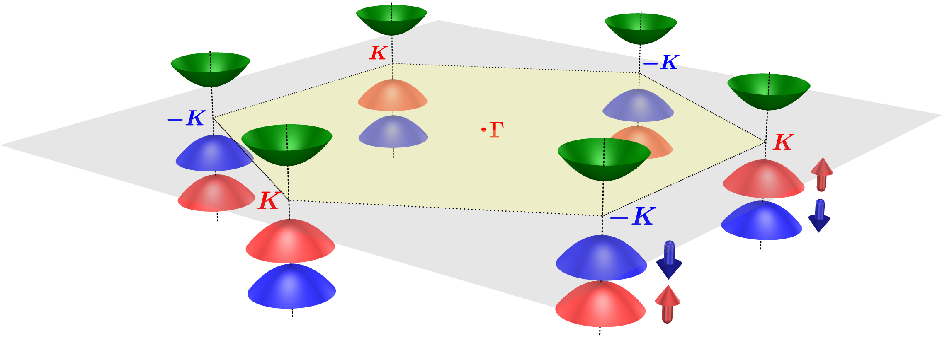
\includegraphics[width=1.0\textwidth]{plots/spin_valley.png}\label{fig:tmd_spin_valley}
            \subcaption{}
        \end{subfigure}
        \caption{Structure of a transition metal dichalcogenide monolayer. (a) Coordination of atoms in a TMD.\@Transition metal (red) is in trigonal prism coordination with chalcogen atoms (blue). (b) Top-view real space structure of a TMD monolayer in 2H phase. (c) Valence band maxima and conduction band minima of a TMD near the K and K' points of the Brillouin zone. Arrows indicate the spin of the electrons.}\label{fig:tmd_general}
    \end{figure}


\begin{figure}[htbp]
    \centering
    \begin{subfigure}[t]{0.55\textwidth}
        \centering
        \includesvg[width=\textwidth]{plots/moire.svg}
        \subcaption{}
        \label{fig:moire_real}
    \end{subfigure}
    \hfill
    \begin{subfigure}[t]{0.4\textwidth}
        \centering
        \includesvg[width=\textwidth]{plots/reciprocal1.svg}
        \subcaption{}
        \label{fig:moire_reciprocal}
    \end{subfigure}
    \caption{TMD --- real and reciprocal space structure, adapted from~\cite{pan2020band}. (a) Real space Moir\'e superlattice of a TMD. The dots in cyan, red and orange indicate $\mathcal{R}_M^M$, $\mathcal{R}_M^X$, $\mathcal{R}_X^M$ local stacking of the atoms (shown in inset). Moir\'e unit cell in blue. (b) Hexagonal Brillouin zone of a metal dichalcogenide monolayer (Red = Top, Blue = Bottom), and a twisted bilayer (Black hexagon), with twist angle $\theta$.}
    \label{fig:moire_structure}
\end{figure}

    TMD monolayers consist of 3 atomic planes --- a middle plane occupied by a transition metal and two outer planes occupied by chalcogen atoms. The two common structural phases are 1T and 2H, from which 2H is the stable one for most of the most commonly studied VI-group TMDs (Fig.~\ref{fig:tmd_struct1}). In 2H phase the transition metal is in a trigonal prism coordination, making up a honeycomb lattice with $\text{D}_\text{3h}$ symmetry (broken inversion symmetry) (Fig.~\ref{fig:tmd_struct2}). Similarly to graphene, the low energy properties can be described in the vicinity of two time-reversal conjugate corners K and -K of the hexagonal 1st Brillouin zone --- the points where the valence band maxima and conduction band minima are located~\cite{coehoorn1987electronic, kormanyos2015k}. It was theoretically modelled by Xiao et al.~\cite{xiao2012coupled} with a two band model, where electrons can be described as massive Dirac fermions. The band structure near the K-points was shown to consist of partially filled d orbitals of the transition metal, with
    \[
     | \phi_c \rangle = | d_{z^2} \rangle, \quad | \phi_v^\tau \rangle = \frac{1}{\sqrt{2}} (| d_{x^2 - y^2} \rangle + i \tau | d_{xy} \rangle)
    \]
    where $\tau = \pm 1$ is the valley index. And $v/c$ subscripts symbolize valence and conduction band respectively. While the conduction band with orbital angular number $L=0$ remains (approximately) spin-degenerate, the valence band built with $L=2$ wavefunctions is split by significant spin-orbit coupling (consequence of broken inversion symmetry), leading to spin-valley locking --- low energy physics of the valence band can be described by a single spin species, with inverse spin in each valley --- thus, the model is time-reversal invariant.
    Due to large distance between valleys in momentum space and due to the spin-valley locking, scattering between the valleys is effectively suppressed. This gives rise to a $U(1) \times U(1)$ symmetry --- charge conservation in each valley, allowing the valley index $\tau$ to be treated as a conserved good quantum number.


    \section{Hall effect and topological order}
        \subsection{Integer Quantum Hall effect}
        \begin{figure}[htbp]
            \centering
            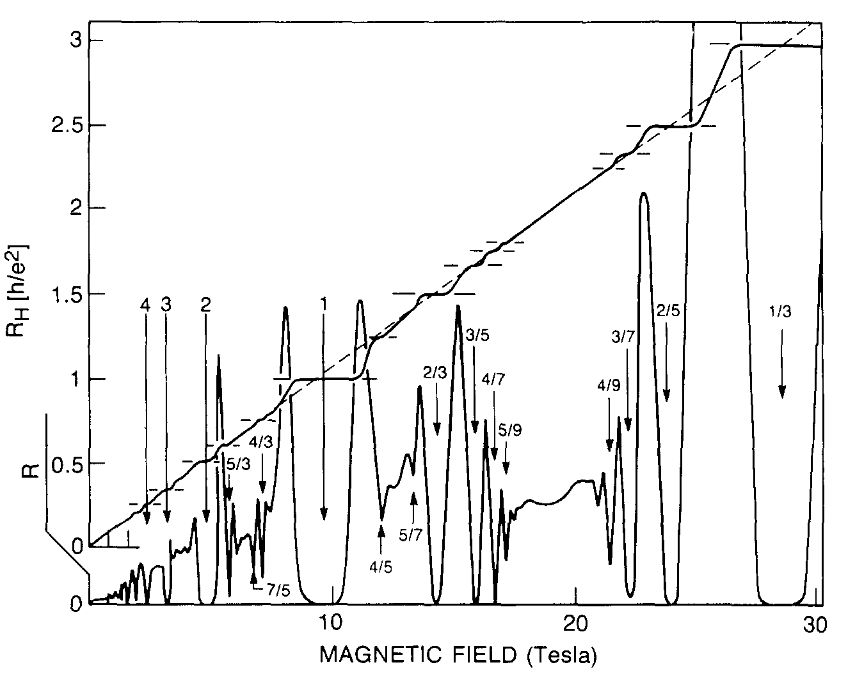
\includegraphics[width=0.5\textwidth]{plots/hall_effect.png}
            \caption{Quantum Hall Effect adapted from~\cite{stormer1992two}.}\label{fig:hall_effect}
        \end{figure}

        The physics of correlated phases in Moir\'e materials has proven in the last years to be very closely related to the physics of the quantum Hall effect --- a phenomenon experienced by a two-dimensional electron system placed in a perpendicular magnetic field, extremely important to the modern condensed matter physics. 
        While classically electrons moving in a 2D system inside a magnetic field simply experience a Lorenz force and and off-diagonal Hall conductivity $\sigma_{xy} \propto B$ can be measured, at low temperatures and in high magnetic fields quantum mechanics comes into play. Quantum mechanically, the magnetic field can be introduced into non-interacting electrons Hamiltonian via the vector potential:
        \[
            \hat{H} = \frac{1}{2m} {\left( \hat{\mathbf{p}} - e \mathbf{A} \right)}^2,\quad B = \nabla \times \mathbf{A}.
        \]
        Introducing appropriate gauge convention (e.g. Landau gauge $\mathbf{A} = (0, Bx, 0)$ or symmetric gauge $\mathbf{A} = (-\frac{1}{2}By, \frac{1}{2}Bx, 0)$), the Schr\"odinger equation can be solved, and the energy spectrum of the system is found to be quantized into equally spaced highly degenerate Landau levels (LLs). The degeneracy, or flatness of Landau levels (LLs) is equivalent to total quenching of the kinetic energy --- similar effect to the one observed in flat Moir\'e bands. This degeneracy of each Landau level is proportional to the number of flux quanta piercing the system, and the filling factor is defined as $\nu = \frac{N_e}{N_\phi}$ where $N_\phi$ is the number of flux quanta and $N_e$ is the number of electrons. In effect, change of the magnetic field changes the filling of LLs.
            Furthermore, via linear response theory, the Hall conductivity can be calculated to take quantized values, dependent directly on the filling $\sigma_{xy} = \nu \frac{e^2}{h},\, \nu \in \mathbb{Z}$, This effect was was discovered in 1980~\cite{von1986quantized} and manifests itself in chracteristic plateaus in the Hall conductivity as a function of magnetic field (Fig.~\ref{fig:hall_effect}). The effect was coined as Integer Quantum Hall Effect (IQHE).
        
        Importantly, physics of IQHE is robust against local disorder and perturbations as it turns out to be topological in nature --- the Hall conductivity can be directly related to the Chern number --- a topological invariant of the system.


        \subsection{Berry phase and Chern number}
        Let
        \[
            \hat{H}(\mathbf{R}(t))
        \]
        be a general Hamiltonian dependent on a time-dependent parameter set $\mathbf{R}(t)$, and
        \[
            \ket{\Psi(0)} = \ket{n(\mathbf{R}(0))}
        \]
        be a non-degenerate eigenstate of the Hamiltonian at time $t=0$, with an energy gap to all other eigenstates.
        The time evolution of the $\ket{\Psi}$ is given by the time-dependent Schr\"odinger equation.
        
        \[
            i \hbar \frac{\partial}{\partial t} \ket{\Psi(t)} = \hat{H}(\mathbf{R}(t)) \ket{\Psi(t)}
        \]
        
        Due to the adiabatic theorem, if the parameters of the Hamiltonian vary slowly enough (with characteristic frequency smaller than the energy gap to other eigenstates), the evolving $\ket{\Psi}$ will remain an instantaneous eigenstate of the Hamiltonian, up to a phase factor
        \[
            \ket{\Psi(t)} = e^{i \gamma(t)} \ket{n(\mathbf{R}(t))}
        \]
        where $\ket{n(\mathbf{R})}$ is the instantaneous eigenstate of the system at time $t$ and $\gamma(t)$ is a phase. Through solving the Schr\"odinger equation, the phase factor is
        \[
            \gamma(t) = -\frac{1}{\hbar} \int_0^t E_n(\mathbf{R}(t')) dt' + \int_{\mathbf{R}(0)}^{\mathbf{R}(t)} \mathbf{A}(\mathbf{R}) \cdot d\mathbf{R}.
        \]

        The first term is a dynamical phase  --- due to the energy of the eigenstate and time evolution itself. The second term is a geometric Berry phase --- it is independent of the time evolution, however, it depends on the path taken in parameter space. The Berry phase can be expressed as a line integral of the Berry connection
        \[
        \mathbf{A}(\mathbf{R}) = i \langle \Psi(\mathbf{R}) | \nabla_\mathbf{R} | \Psi(\mathbf{R}) \rangle
        \]
        Additionally, the Berry curvature is defined as $\mathbf{\Omega}(\mathbf{R}) = \nabla_\mathbf{R} \times \mathbf{A}(\mathbf{R})$.
        Importantly when the path taken in the parameter space is closed, the system returns to its initial state, thus, the Berry phase can only differ by a multiple of $2\pi$. The Berry curvature can be expressed as a surface integral of the Berry curvature over the surface enclosed by the path, $\gamma = \int_S \mathbf{\Omega}(\mathbf{R}) \cdot d\mathbf{S} = 2\pi C$, where $C$ is the Chern number taking integer values. The Chern number is a topological invariant of the system --- since it takes integer values it cannot change continuously, and it can change only when the gap of the system closes. While in general Berry phase is gauge dependent, when the path is closed, Berry phase and thus Chern number are both gauge invariant quantities.. As such it is robust against perturbations. While the notion introduced here is general, in the case of electrons in magnetic field, the Berry curvature corresponds to the magnetic field, the Berry connection to its vector potential, the Berry phase to the Aharonov-Bohm phase and the Chern number to the number of flux quanta piercing the system. Using linear response theory, the Chern number can be shown to be directly related to the Hall conductivity, $\sigma_{xy} = C \frac{e^2}{h}$, so in this case $C = \nu$.~\cite{tong2016lectures}

        These notions can be generalized to treat a degenerate subspace --- the Berry connection becomes a matrix over the degenerate subspace, and the \textit{First} Chern number (which now is one of a bigger group of topological invariants) is defined as $C_1 = \frac{1}{2\pi} \int_S \text{Tr}(\mathbf{\Omega}(\mathbf{R})) \cdot d\mathbf{S}$, where $\mathbf{\Omega}(\mathbf{R}) = \nabla_\mathbf{R} \times \mathbf{A}(\mathbf{R}) - i \mathbf{A}(\mathbf{R}) \times \mathbf{A}(\mathbf{R})$ is the non-abelian Berry curvature.~\cite{tong2016lectures}




        \subsection{Fractional quantum hall effect}
        In clean samples at strong magnetic fields, additional quantum Hall plateaus were detected --- at magnetic fields corresponding to fractional fillings of Landau levels --- effect coined as Fractional Quantum Hall Effect (FQHE) (Fig.~\ref{fig:hall_effect}). While IQHE can be explained by non-interacting electrons, the FQHE is a direct consequence of electron-electron interaction. Such interaction breaks the degeneracy of many-body states within LLs.
        
        Similarly, to IQHE, the FQHE can be related to the (first) Chern number, however the degeneracy of the fractional state has to be taken into account.
        
        The most notable plateaus reside at filling of $\nu = \frac{1}{q}$ with $q \in \mathbb{N_{\text{odd}}}$ (Fig.~\ref{fig:hall_effect}). While an analytical explanation is intractable for Coulomb interaction, an ansatz wavefunction --- Laughlin wavefunction~\cite{laughlin1983anomalous} --- was shown to capture the essential physics. While it is strictly the exact ground state of a simplified pseudopotential Hamiltonian, numerical studies have shown it maintains a remarkably high overlap with the ground states of realistic interactions.

        For such states, and more generally for filling $\nu = \frac{p}{q},\, p\in \mathbb{N},\, q\in \mathbb{N}_{\text{odd}},\,\gcd(p, q) = 1$, due to the algebra of (magnetic translation) operators~\cite{bernevig2012emergent}, the ground state degeneracy is $q^g$ where g is the genus of the manifold under study. A common choice, used also in this thesis, is a torus with $g=1$. Due to the non-abelian Berry connection construction, each of the degenerate states contributes equally to the Chern number and to the Hall conductivity, resulting in the fractional quantization of the Hall conductivity $\sigma_{xy} = \frac{1}{q} \frac{e^2}{h}$ for each of the ground states.
        
        Beyond quantized conductivity, the FQHE is also characterized by the presence of anyonic excitations --- the elementary quasiparticle and quasihole excitations can possess fractional charge (fraction of the charge of an electron), and fractional statistics.
        During a spatial exchange of two quasiparticles, due to their indistinguishability, their wavefunction can only change by a phase factor, $\Psi \to e^{i \theta} \Psi$. For fermions the phase is $\pi$ corresponding to a minus sign, while for bosons the phase is $0$. In 3D, if one particle takes a path around the other and returns to its starting position, the path can be continuously deformed to one where the particle does not move --- thus, double the phase factor has to be a multiple of $2\pi$. However, in 2D this is not the case --- a closed path encompassing another particle is topologically distinct from one that does not encompass any. Thus, the end state need not have the same phase as the starting state, and the exchange phase factor can take any value $\theta \in [0, 2\pi)$. The quasiparticles acquiring this general phase are called abelian anyons.
        However, if the Hilbert space of a single quasiparticle has more than one dimension, the exchange of two quasiparticles can correspond to a more general unitary transformation $\mathbf{U}$ in this local space $\Psi \to \mathbf{U} \Psi$. In this case, the exchange of different particles is non-commutative, and they are \textit{non-abelian} anyons. Since the topological nature of the FQHE is robust against perturbations, the anyonic statistics of the quasiparticles inherits this trait. This makes such topological materials favorable for topological quantum computing --- a notion of using the non-abelian anyons as qubits, where execution of quantum gates would correspond to simple spatial exchanges of the anyons --- ``braiding''~\cite{das2005topologically, nayak2008non}.

        In this aspect, Laughlin states in a FQH system have abelian statistics with the exchange phase $\theta = \frac{\pi}{q}$ for $\nu = \frac{1}{q}$.


\subsection{Composite fermions and the composite Fermi liquid}

    A complementary picture of the fractional quantum Hall effect (FQHE), particularly at even-denominator fillings such as $\nu = \frac{1}{2}$, is provided by composite fermions~\cite{jain1989composite}. In this framework, each electron binds an even number $2p$ of magnetic flux quanta, forming emergent fermionic quasiparticles. This flux attachment can be implemented formally via a singular gauge transformation, providing a mean-field description where the electrons are viewed as composite fermions moving in a reduced effective field
    \begin{equation}
        B_{\mathrm{eff}} = B - 2p\phi_0 n_e,
    \end{equation}
    where $n_e$ is the electron density and $\phi_0 = h/e$ is the flux quantum.
    At filling fractions
    \begin{equation}
        \nu = \frac{p}{2p \pm 1},
    \end{equation}
    the composite fermions fill an integer number of their own effective Landau levels, reinterpreting the FQHE of electrons as an integer quantum Hall effect of composite fermions~\cite{jain1989composite}.

    At the special filling $\nu = 1/2$ (and more generally $\nu = 1/(2p)$), the attached flux effectively cancels the external magnetic field ($B_{\mathrm{eff}} \to 0$), and composite fermions form a compressible, metallic state known as the composite Fermi liquid (CFL). This is confirmed by a definite lack of a plateau in the Hall conductivity at $\nu = 1/2$, in Fig.~\ref{fig:hall_effect}.

        \subsection{Higher Landau levels and non-abelian states}
        While non-abelian states can in principle be found in lowest Landau level, they have been shown to be mostly unattainable with Coulomb interaction\cite{storni2010fractional}. They are, however, found in higher Landau levels e.g. a prominent Hall plateau at $\nu = \frac{5}{2}$ (Fig,~\ref{fig:hall_effect})~\cite{willett1987observation}. 
        As an explanation, an ansatz Moore-Read wavefunction was soon devised~\cite{MOORE1991362}. Like Laughlin wavefunction, it is a ground state of a specific Hamiltonian, however, here the Hamiltonian is composed of 3-body interaction. It was shown numerically to be a good description of the ground state of quantum hall Hamiltonian at $\nu=\frac{5}{2}$. It is worth noting that this notation corresponds not to the half filling of $n=2$ landau level, but to the filling of the lowest Landau level by two spin species, and half filling of the $n=1$ Landau level by one of the species.
        For Coulomb interaction the state is not very robust --- lying close to competing phases --- and the interaction needs to be fine-tuned to stabilize the state~\cite{PhysRevLett.84.4685}.
        
        As Moore-Read state can be understood in terms of Cooper pairing of composite fermions, its ground state degeneracy shows characteristic dependence on the parity of the number of fermions in the system. For a genus $g$ manifold it is shown to be $3(M+1)^g$ for even number of fermions and $3M^g$ for odd number of fermions, where $M$ comes from the filling fraction $\nu=\frac{1}{M+1}$~\cite{bernevig2012emergent}.
        For states studied in the thesis, $g=1$ (torus/PBC) and $M=1\,(\nu=\frac{1}{2})$, expecting degeneracy of 6 and 2 for even and odd number of fermions respectively.~\cite{read2000paired, oshikawa2006fractionalization}

        \subsection{Spectral flow}
        In IQH system with periodic boundary conditions (on a torus), an additional magnetic flux can be inserted into the system through one of the cycles of the torus.
        Such flux insertion affects the energy spectrum of electrons --- effectively modifying the boundary condition while solving for the eigenstates of the system. It can be found, however, that the insertion of an integer number of flux quanta has to leave the spectrum invariant as it can be gauged away. Crucially equality of the spectrum does not mean equality of the eigenstates. Using the magnetic translation operators it was shown that --- the states permute within the degenerate ground state manifold under flux insertion --- a phenomenon called spectral flow.

        The ground state degeneracy and spectral flow were shown to be sufficient conditions to identify a topological nature of phases of matter if the spectral gap does not close in thermodynamic limit~\cite{regnault2011fractional}.


        \section{Topology of Moire materials}

        While the QHE stems from strong magnetic fields, its topological description in terms of Chern number does strictly require them. Impracticality of such strong fields led to a question of whether topological states can be realized in two-dimensional systems without a net magnetic field. First lattice models achieving that~\cite{PhysRevLett.61.2015} introduced explicit time reversal symmetry breaking by introducing a complex hopping term which effectively acts as an analogue of magnetic field and Aharonov-Bohm phase related to it. In result, for a specific parameter range the system's band structure possesses non-zero Chern number. This was later generalized to a more realistic model of graphene~\cite{PhysRevLett.95.226801}. Where the non-trivial hopping amplitude is directly caused by spin-orbit coupling.

        A topologically non-trivial phase with a non-zero Chern number that exhibits the integer or fractional quantum Hall effect without an external magnetic field is known as a Chern Insulator (CI) or Fractional Chern Insulator (FCI), respectively. Although these systems exhibit quantum Hall behavior, they explicitly break time-reversal symmetry. An analogous time-reversal-invariant state can be constructed by combining two time-reversed copies of a Chern insulator with opposite Chern numbers. Because the total Chern number vanishes and time-reversal symmetry is preserved, the net charge Hall conductance is zero. However, if the spin component $s_z$ is a conserved quantity, the system can exhibit a spin quantum Hall effect, where opposite spin channels carry counter-propagating currents with opposite conductances. In the more general case where spin conservation is broken by spin-orbit coupling, the system transitions into a topological insulator (TI), or a fractional topological insulator (FTI).  

    A similar mechanism operates in the effective continuum model of group-VI transition metal dichalcogenides in the $2H$ phase. Near the high-symmetry points $K$ and $-K$, the low-energy physics is described by a massive Dirac Hamiltonian:
    \[
        \hat{H}(\mathbf{k}) = \mathbf{\Delta}(\mathbf{k}) \cdot \mathbf{\hat{\sigma}}
    \]\cite{xiao2012coupled}
    This is analogous to a two-level system in a magnetic field, where the vector $\mathbf{\Delta}(\mathbf{k})$ corresponds to the magnetic field. Here, however, $\mathbf{\Delta}(\mathbf{k})$ acts as a valley pseudospin driven directly by strong spin-orbit coupling.As in the standard description of the Berry phase and Chern number, this two-level Hamiltonian is parametrized by momentum. The Chern number of its eigenstates can be calculated directly by treating the momentum components as parameters. Depending on the sign of the effective mass term, the Chern number of the valence band is $C = \pm 1$ for the $K$ and $-K$ valleys, respectively. In a multi-band continuum model, the global topology of the bands depends strongly on the twist angle. For $\text{MoTe}_2$ at a twist angle of $\theta \approx 1.89^\circ$, for example, it has been found that the two highest occupied bands and the conduction band all possess $C = 1$ and, combined with their flat dispersion, can closely emulate the physics of the three lowest Landau levels~\cite{xu2025multiple, li2025variational}.Consequently, Moir\'e materials provide an exceptionally promising platform for realizing topological phases of matter—including time-reversal-invariant topological insulators and fractional Chern insulators (FCIs) --- by leveraging the presence of two naturally time-reversal-conjugate valleys.


    \chapter{Model}\label{ch:model}
    The model used here is designed to emulate Moir\'e materials and is based on the work of Kwan et al.~\cite{kwan2025textured}. As motivated in \S\ref{sec:moire_topology}, the two valleys of a Moir\'e TMD carry opposite Chern number and can, near the relevant magic angle, closely emulate a pair of oppositely oriented Landau levels; we take this correspondence as the starting point of the model. For simplicity of implementation and interpretation, we work on a square lattice with lattice constant $a = \sqrt{2\pi}$, in units where the magnetic length is $l_B = 1$ and there is one flux quantum per unit cell. The magnitude of the primitive reciprocal lattice vector is then $Q = 2\pi/a = a = \sqrt{2\pi}$. The single-particle Hilbert space consists of two Landau levels carrying a valley index $\tau = \pm 1$, which experience opposite effective magnetic fields $B_\tau = \tau B$. To represent a generic Moir\'e material, the model combines a screened Coulomb interaction projected onto a single Landau level (i.e., neglecting Landau-level mixing) with a single-particle potential representing the Moir\'e potential of the real material. We work on a torus (periodic boundary conditions) and treat the magnetic vector potential in the periodic gauge. Relative to the original formulation of Kwan et al., the model is additionally modified to allow projection onto higher Landau levels, and to allow for an inverted single-particle dispersion in one of the two valleys.

\section{Interactions}\label{sec:interactions}
The interaction is modeled as a screened Coulomb density-density interaction projected onto the Landau level, with a tunable inter-valley coupling strength:
\begin{equation}
    H_{\text{int}} = \frac{1}{2A} \sum_{\substack{\mathbf{k} \in \text{BZ} \\ \mathbf{k}' \in \text{BZ} \\ \mathbf{q}}} \tilde{U}_{\tau \tau'}(\mathbf{q}) \, \Lambda_\tau(\mathbf{k}, \mathbf{q}) \, \Lambda_{\tau'}(\mathbf{k}', -\mathbf{q}) \, d^\dagger_{\mathbf{k}, \tau} \, d^\dagger_{\mathbf{k}', \tau'} \, d_{\lfloor \mathbf{k}' - \mathbf{q} \rfloor, \tau'} \, d_{\lfloor \mathbf{k} + \mathbf{q} \rfloor, \tau},
    \label{eq:interaction}
\end{equation}
where $A$ is the area of the system, $\tau, \tau'$ is the valley index and
\begin{equation}
    \tilde{U}_{\tau \tau'}(\mathbf{q}) = \frac{2\pi}{q (1 + l_{\text{RK}} q)} \tanh(q \, d_{\text{SC}}) \, (1 + \alpha \, \tau \tau')
    \label{eq:interaction_potential}
\end{equation}
is the interaction potential. The $l_{\text{RK}} = 0$ limit of Eq.~\eqref{eq:interaction_potential} is the screened Coulomb interaction of a charge held midway between two perfectly conducting plates separated by a distance $d_{\text{SC}}$. The Rytova--Keldysh correction $l_{\text{RK}} \neq 0$ additionally accounts for the dielectric environment and the polarizability of the sample itself~\cite{rytova2018screened, keldysh2024coulomb, cudazzo2011dielectric}. The parameter $\alpha \in [-1, 1]$ controls the relative strength of inter- and intra-valley interactions and is central to the calculations that follow: at $\alpha = 0$ the interaction is valley-isotropic with $\tilde{U}_{+, -} = \tilde{U}_{-, +} = \tilde{U}_{+, +} = \tilde{U}_{-, -}$; at $\alpha = 1$ only the intra-valley interaction survives, $\tilde{U}_{+, -} = \tilde{U}_{-, +} = 0$; and at $\alpha = -1$ only the inter-valley interaction survives.

The interaction is projected onto a Landau level through the form factor $\Lambda$, which, in the periodic gauge with $\mathbf{k} \in [0, Q) \times [0, Q)$ (the Brillouin zone), takes the following form for the lowest Landau level:
\begin{equation}
    \Lambda_\tau(\mathbf{k}, \mathbf{q}) = e^{-|\mathbf{q}|^2/4} \, e^{-i \tau \left( -q_x (k_y + q_y/2) \, - \, k_x k_y \, + \, \lfloor k_x + q_x \rfloor (k_y + q_y) \right)}
    \label{eq:form_factor_lll}
\end{equation}
following Kwan et al.~\cite{kwan2025textured}. Abouelkomsan and Fu~\cite{abouelkomsan2025non} further showed that projecting the interaction onto higher Landau levels amounts, in this formalism, to multiplying the lowest-Landau-level form factor by the Laguerre polynomial $L_n$ of the corresponding Landau-level index $n$:
\begin{equation}
    \Lambda_{n, \, \tau}(\mathbf{k}, \mathbf{q}) = \Lambda_\tau(\mathbf{k}, \mathbf{q}) \, L_n\!\left( \frac{|\mathbf{q}|^2}{2} \right).
    \label{eq:form_factor_general}
\end{equation}
The two Laguerre polynomials relevant to this work are $L_0(x) = 1$ and $L_1(x) = 1-x$, corresponding respectively to the lowest Landau level (LLL, $n=0$) and the first excited Landau level (1LL, $n=1$). The operator $\lfloor \cdot \rfloor$ denotes reduction modulo $Q$, mapping momenta back into the Brillouin zone.

Throughout this work we consider two variants of the interaction potential $\tilde{U}_{\tau \tau'}(\mathbf{q})$ defined in Eq.~\eqref{eq:interaction_potential}: the full interaction as given above, matching Kwan et al.~\cite{kwan2025textured}, and a modified variant with $\tilde{U}_{\tau \tau'}(\mathbf{q} = 0) = 0$ for all $\tau, \tau'$. 

\checkthis{The $U(q=0)=0$ might in fact be wrong -that's why I haven't described some of the results with it later on in the thesis. Going through the calculations, the fact that should be subtracted from the q=0 part I believe, could be only the part that couples to the total charge density, rather than the full q=0 component. The same is done in~\cite{abouelkomsan2025non}. Doing this in fact only shifts the \textit{total} energies of all of the states by a constant but the \textit{relative} energies of all the momentum sectors are unchanged. Which means, the ``normal'' interaction version would be a correct one anyway.}

\section{Single-particle dispersion}
The single-particle dispersion is modeled as a lowest-harmonic cosine potential, compatible with the choice of the magnetic unit cell, following Kwan et al.~\cite{PhysRevLett.124.166601} and Bultinck et al.~\cite{PhysRevLett.124.166601}:
\begin{equation}
    \epsilon_\tau(\mathbf{k}) = -\frac{W}{4} \left( \cos(k_x a) + \cos(k_y a) \right) \cdot \tau^{(1 - \mathrm{sgn}(W))/2}.
    \label{eq:dispersion}
\end{equation}
Relative to these references, we introduce the valley-dependent prefactor $\tau^{(1-\mathrm{sgn}(W))/2}$, which allows for an inverted dispersion in one of the two valleys. For $W>0$ the prefactor is $\tau^0=1$ and Eq.~\eqref{eq:dispersion} reduces to the same dispersion in both valleys, as in the original model; for $W<0$ the prefactor becomes $\tau^1 = \tau$, so that the dispersion is inverted in one of the valleys relative to the other.



  \chapter{Methods}\label{ch:methods}
    Having introduced the model Hamiltonian in Chapter~\ref{ch:model}, we now describe how it is solved numerically. All results in Chapter~\ref{ch:results}~and~\ref{ch:results_1LL} are obtained by exact diagonalization (ED) on finite tori, using the criteria for identifying topological order laid out at the end of this chapter.

\section{Exact diagonalization}\label{sec:ed}

The model Hamiltonian is solved using the DiagHam package for exact diagonalization~\cite{DiagHam}. On a torus geometry (periodic boundary conditions), the center-of-mass (COM) momentum is a good quantum number~\cite{bernevig2012emergent}, which allows an initial block-diagonalization of the Hamiltonian into sectors labeled by  the COM momentum $\mathbf{K} = (K_x, K_y)$, and the valley polarization $P_z = N_+ - N_-$ ($N_\tau$ being the occupation of the $\tau$ valley). Within each block, the Hamiltonian matrix is constructed explicitly, and its lowest few eigenvalues are found iteratively using the Lanczos algorithm~\cite{Lanczos1950}. The number of eigenvalues requested in each sector is chosen to exceed the maximum ground-state degeneracy expected for the filling under consideration.

\section{Momentum grid discretization and tilted boundary conditions}\label{sec:tilted_bc}

To construct the finite Hamiltonian matrix, the Brillouin zone $[0, Q) \times [0, Q)$ must be discretized into a finite set of momentum points. This grid is not unique: as shown by L\"auchli et al.~\cite{lauchli2013hierarchy} and Repellin et al.~\cite{repellin2014z} in the context of fractional Chern insulators, different admissible choices of a real-space cluster correspond to very different sampling of the same Brillouin zone, and this choice can noticeably affect the stability of the resulting topological phases.

The grid is constructed by first choosing two real-space spanning vectors,
\begin{equation}
    \mathbf{T}_1 = n_{x1}\mathbf{a}_1 + n_{y1}\mathbf{a}_2, \qquad
    \mathbf{T}_2 = n_{x2}\mathbf{a}_1 + n_{y2}\mathbf{a}_2,
    \label{eq:tilted_vectors}
\end{equation}
with integer coefficients $n_{x1}, n_{y1}, n_{x2}, n_{y2}$, where $\mathbf{a}_1, \mathbf{a}_2$ are the primitive lattice vectors of the underlying square lattice. These two vectors define the finite cluster on which the many-body problem is solved, enclosing $N_\phi = |n_{x1}n_{y2} - n_{x2}n_{y1}|$ unit cells (flux quanta).

Invariance of the many-body wavefunction under a translation by $\mathbf{T}_1$ or $\mathbf{T}_2$ forces the single-particle momentum $\mathbf{k}$ to satisfy $\mathbf{k}\cdot\mathbf{T}_1, \, \mathbf{k}\cdot\mathbf{T}_2 \in 2\pi\mathbb{Z}$. Equivalently, $\mathbf{k}$ must lie on the lattice spanned by the reciprocal vectors $\tilde{\mathbf{T}}_1, \tilde{\mathbf{T}}_2$ dual to $\mathbf{T}_1, \mathbf{T}_2$,
\begin{equation}
    \tilde{\mathbf{T}}_i \cdot \mathbf{T}_j = 2\pi \delta_{ij}, \qquad i,j = 1,2.
    \label{eq:dual_vectors}
\end{equation}
The admissible momenta are the $N_\phi$ points of this reciprocal lattice that fall within one Brillouin zone, i.e.\ they are defined modulo $\tilde{\mathbf{a}}_1$ and $\tilde{\mathbf{a}}_2$ (reciprocal vectors dual to $\mathbf{a}_1, \mathbf{a}_2$: $\tilde{\mathbf{a}}_i \cdot \mathbf{a}_j = 2\pi \delta_{ij}$). Concretely, we label them by two integers $(p,q)$,
\begin{equation}
    \mathbf{k}_{p,q} = p\,\tilde{\mathbf{T}}_1 + q\,\tilde{\mathbf{T}}_2 \pmod{\tilde{\mathbf{a}}_1, \tilde{\mathbf{a}}_2},
    \label{eq:tilted_momenta}
\end{equation}
choosing $p \in [0, N_1)$ and $q \in [0, N_2)$ with $N_1 N_2 = N_\phi$, such that every point is counted exactly once and no two choices of $(p,q)$ give equivalent momenta. In practice this means imposing $N_i\tilde{\mathbf{T}}_i \equiv 0 \pmod{\tilde{\mathbf{a}}_1,\tilde{\mathbf{a}}_2},\, i\in \{ 1,\,2\}$, and wrapping $\mathbf{k}_{p,q}$ back into the first BZ whenever it falls outside of it.


For a fixed $N_\phi$, this construction allows much more freedom in choosing the cluster shape than an untilted grid. L\"auchli et al.~\cite{lauchli2013hierarchy} mention that clusters with $|\mathbf{T}_1|/|\mathbf{T}_2| \gg 1$ tend to favor charge-density-wave states over the target topological phase; this was the main criterion used here for selecting the tilting, i.e.\ $\mathbf{T}_1, \mathbf{T}_2$ were chosen so that $|\mathbf{T}_1|/|\mathbf{T}_2|$ is as close to $1$ as possible. Among the remaining choices with comparable aspect ratio, the angle between $\mathbf{T}_1$ and $\mathbf{T}_2$ was further chosen to be as close as possible to $60^\circ$ (equivalently $120^\circ$), so that the resulting momentum-space sampling is most isotropic, i.e.\ closest to a uniform hexagonal grid.

For simplicity, however, unless stated otherwise, the calculations presented in this thesis use the conventional (untilted) boundary conditions $\mathbf{T}_i = N_i\mathbf{a}_i$, corresponding to a rectangular grid of momenta in the Brillouin zone. Tilted boundary conditions are used only where explicitly noted, primarily for the momentum-occupation calculations of Chapter~\ref{ch:results}, and in Chapter~\ref{ch:results_1LL}, where less stable non-abelian phases are expected.
\section{Twisted boundary conditions and flux insertion}\label{sec:flux_insertion}

To explicitly check for spectral flow, twisted boundary conditions are used, whereby an additional flux $\mathbf{\Phi} = (\Phi_1, \Phi_2)$ is inserted into the system through the two cycles of the torus. Because the two valleys experience opposite effective magnetic field (and carry opposite Chern number $C = \tau$), the flux is inserted with opposite sign in the two valleys,
\begin{equation}
    \mathbf{\Phi}_\tau = \tau\, \mathbf{\Phi}.
\label{eq:flux_valley_sign}
\end{equation}
This is equivalent to an effective uniform, valley-dependent shift of the momentum grid sampled in the Hamiltonian,
\begin{equation}
    \mathbf{k}_\tau = \mathbf{k}^0 + \tau\frac{\Phi_1}{2\pi} \tilde{\mathbf{T}}_1 + \tau\frac{\Phi_2}{2\pi} \tilde{\mathbf{T}}_2
\label{eq:flux_shift}
\end{equation}
where $\mathbf{k}^0$ is the original (untwisted) momentum. Here, $\Phi_i = 2\pi$ corresponds to one flux quantum --- it shifts the momentum grid by exactly one grid step in the corresponding direction, which further shows that the spectrum must be identical at $\Phi_i = 0$ and $\Phi_i = 2\pi$: the twisted grid coincides with the original one, merely relabeled.

This valley-antisymmetric choice is what makes flux insertion compatible with the symmetries of the Hamiltonian: time-reversal symmetry $\hat{T}$ at $W>0$ and the combined symmetry $\hat{C}\hat{T}\hat{C}^{-1}$ of \S\ref{sec:symmetries} at $W<0$.

Throughout the thesis the flux is inserted along $\tilde{\mathbf{T}}_1$ ($\Phi_2 = 0$), which corresponds to the $x$ axis for the untilted boundary conditions.

\section{Numerical identification of topological phases}\label{sec:recognition}

The nature of each ground-state phase is determined from the following characteristics.

First, the ground-state valley polarization is identified as the $P_z$ sector containing the lowest-energy eigenstate.

Second, the gaps between consecutive energy levels are computed. Exact diagonalization is performed for $10$ equally spaced flux values $\phi \in [0,2\pi]$. For a candidate $N$-fold degenerate ground-state manifold, we define the spectral gap as
\begin{equation}
    \Delta_N =
    \begin{cases}
        \min_{\phi} E_{N+1}(\phi) - \max_{\phi} E_N(\phi), & \text{if } {\{\mathbf{k}_n(\phi_1)\}}_{n=1}^{N} = {\{\mathbf{k}_n(\phi_2)\}}_{n=1}^{N} \ \ \forall\, \phi_1, \phi_2 \in [0, 2\pi], \\[4pt]
        0 & \text{otherwise.}
    \end{cases}
    \label{eq:spectral_gap}
\end{equation}
The gap is evaluated for every $N$ relevant to the filling under consideration. Here, $E_N(\phi)$ denotes the energy of the $N$-th state at flux $\phi$, with the spectrum ranked across all center-of-mass momentum and valley-polarization sectors, and $\mathbf{k}_n(\phi)$ denotes the center-of-mass momentum of that state. The spectral gap is therefore determined by the separation between the highest energy attained by the candidate ground-state manifold and the lowest energy attained by the first excited state over the full flux interval. This ensures that the entire $N$-fold manifold remains separated from higher-energy states throughout flux insertion. The second condition sets the gap to zero if the set of COM momenta spanning the candidate ground-state manifold changes with flux, which signals a level crossing between the candidate manifold and a state outside it and hence a closing of the gap.

Third, the variation of spectra under flux insertion is inspected visually for spectral flow between the states within the ground-state manifold.

As discussed in Chapter~\ref{ch:introduction}, spectral flow, ground-state degeneracy, and the absence of gap closing in the thermodynamic limit together constitute strong evidence for a gapped topological phase. Thus, additionally to probes above, a fully rigorous identification would require finite-size scaling. Due to the limited computational resources, such a systematic scaling analysis was not performed; the results presented here should therefore be understood as consistent with, rather than a definitive proof of, the identified phases.

Finally, for some systems the momentum-space occupation $n(\mathbf{k}) = |\langle \mathbf{k} | \psi_0 \rangle|^2$ of the ground state at zero flux is additionally computed, in order to distinguish the flat occupation characteristic of topological states (e.g.\ FCIs) or of gapless composite-Fermi-liquid-like states from the peaked occupation expected of a Fermi liquid.

The description of numerical criteria used for each phase is deferred until after the discussion of suspected phases at different fillings, and is done in Table~\ref{tab:lll-phases} for the LLL and Table~\ref{tab:1ll-phases} for the $n=1$ LL.

It is also worth noting that due to the lack of inter-valley tunneling in the model, the inter-valley coherence order parameter $\langle d^\dagger_{k,+} d_{k',-} \rangle$ is identically zero in all calculations, and hence cannot be directly used.

    \chapter{Results --- lowest Landau level}\label{ch:results}
    We now turn to results for the lowest Landau level. Phase-diagram calculations (ground-state valley polarization, spectral gaps, and flux insertion) are performed on a $3\times4$ system with the default (untilted) Brillouin-zone sampling, scanning $W$ and $\alpha$. The momentum-occupation calculations are instead performed on a tilted lattice, with the Brillouin-zone sampling shown in Fig.~\ref{fig:half_half_density_CFL}. Unless stated otherwise, $d_{\text{SC}} = 6a$ and $l_{\text{RK}} = 0$ are used as default parameters, following Kwan et al.~\cite{kwan2024could}.

To connect with previous theoretical and experimental work, and because they are the fillings at which topological phases are expected, we consider $\nu = \tfrac{1}{2}$, $\nu = \tfrac{2}{3}$, and $\nu = 1$.

\section{Anticipated phases}

\subsection{\texorpdfstring{$\nu = \frac{2}{3}$}{nu = 2/3} (\texorpdfstring{$\nu=\frac{1}{3}$}{nu = 1/3} per valley)}

At the decoupled limit $\alpha = 1$, $W=0$, the intra-valley repulsion favors a valley-unpolarized $\tfrac{1}{3} + \tfrac{1}{3}$ state, and the ground state is expected to be a fractional topological insulator (FTI) consisting of two time-reversal-conjugate copies of the Laughlin $\tfrac{1}{3}$ state, $\ket{\text{FTI}} = \ket{\text{FQH}} \otimes \overline{\ket{\text{FQH}}}$ (with overline denoting time-reversal conjugate state), with a characteristic $3\times 3 = 9$-fold ground-state degeneracy on the torus~\cite{chen2012interaction}. At low $\alpha$, the large inter-valley interaction should instead favor a valley-polarized phase, with a $\nu = \tfrac{2}{3}$ Laughlin-type fractional quantum Hall (FQH) state expected in a single valley, consistent with prior theoretical work at the same filling~\cite{crepel2023anomalous}. Experimentally, fractional Chern insulator states have been reported in twisted MoTe$_2$ at closely related fillings~\cite{cai2023signatures, xu2023observation, zeng2023thermodynamic, park2023observation}, supporting this general picture.

The nature of the states and transitions connecting the FQH and FTI phases as $\alpha$ is tuned is not well understood \emph{a priori}. Near the decoupled limit $\alpha \to 1$, McDonald and Haldane~\cite{mcdonald1996topological} studied a closely related problem of two-component quantum Hall states at $\nu_T = 2/3$ using a $K$-matrix Chern--Simons description, and found that increasing the inter-component coupling drives a transition from the decoupled $(3,3,0)$-type state (equivalent to our FTI) to a competing $(1,1,2)$ Halperin state. However, contrary to the literature, our two valleys carry opposite Chern number --- the standard holomorphic Halperin $(m,n,l)$ wavefunction construction does not directly apply. % chktex 8

Independently, the bandwidth $W$ is expected to compete against these interaction-favored ordered states: in the limit $W \to \infty$, kinetic energy favors a gapless, valley-unpolarized Fermi liquid ($\mathrm{FL}_{\text{unpol.}}$) state, so transitions that destroy both the valley polarization and the topological order of the low--$\alpha$ phases (FTI, FQH) are expected. While the nature of transitions out of gapped topological states has not been addressed in the literature, the valley-depolarization transition is expected to be Stoner-like and was treated with a mean-field approach in Ref.~\cite{raines2024unconventional}. That reference also notes that, depending on the inter-valley coupling, a similar Stoner mechanism can instead drive an FL$\to$inter-valley-coherent (IVC) transition rather than valley polarization; the IVC state is therefore also a candidate phase at intermediate $\alpha$.

\subsection{\texorpdfstring{$\nu = 1$}{nu = 1} (\texorpdfstring{$\nu=\frac{1}{2}$}{nu = 1/2} per valley)}

At $\alpha = 1$, $W = 0$, the ground state is expected to be a pair of decoupled composite Fermi liquids, $\ket{\text{CFL}} \otimes \overline{\ket{\text{CFL}}}$, consistent with exact-diagonalization studies of the continuum MoTe$_2$ model at the same filling~\cite{dong2023composite}.

At small $\alpha$, valley polarization is again expected, giving an integer quantum Hall (IQH) state. Since it corresponds to integer filling of the LLL, the Hilbert space at full valley-polarization is one-dimensional, and no other state is possible in this region. As before, increasing $|W|$ is expected to drive a Stoner-like depolarization transition to an $\mathrm{FL}_u$ state. Consistently with the Stoner treatment of Ref.~\cite{raines2024unconventional}, an IVC state is additionally expected to appear at intermediate $\alpha$, again transitioning to an $\mathrm{FL}_\mathrm{unpol.}$ state at large $|W|$. This IVC state was found directly in a Hartree--Fock treatment of the same model, in Ref.~\cite{kwan2025textured}. The transition between the IVC state and the decoupled CFL pair as $\alpha$ increases, however, has not been directly addressed in the literature. % chktex 8

The two-valley LLL and 1LL model was also studied by Das, Wagner, and Neupert~\cite{das2025fractional}. By tuning the Haldane pseudopotentials, they found phases similar to the ones described above, in addition to partially particle--hole-transformed Halperin states. % chktex 8

\subsection{\texorpdfstring{$\nu = \tfrac{1}{2}$}{nu = 1/2} (\texorpdfstring{$\nu=\frac{1}{4}$}{nu = 1/4} per valley)}

We do not expect a gapped topological phase at this filling. By analogy with $\nu=1$, a composite-Fermi-liquid state $\ket{\text{CFL}} \otimes \overline{\ket{\text{CFL}}}$ is expected at $\alpha=1$, and a single valley-polarized CFL (denoted by $\ket{\text{CFL}}_{\text{pol.}}$) is expected at low $\alpha$ in the valley-polarized region, with both giving way to a Fermi liquid at large $|W|$. We are not aware of prior literature directly addressing this specific filling.


\subsection{Numerical criteria for defining phases}
As the thesis focuses on gapped topological FQH and FTI phases, the main phase diagrams shown in this chapter use only a general distinction of phases based on valley polarization, spectral gap, and presence of spectral flow, for both $U(\mathbf{q} = 0)=0$ and $U(\mathbf{q}=0)\neq0$ interactions. In this way, however, separate non-topological phases are not resolved and are covered under the umbrella labels ``UP'' (unpolarized) and ``VP'' (polarized), as shown in Table~\ref{tab:lll-phases}a. For $U(\mathbf{q}=0)\neq0$, these regions are described in more detail in the text and in the summary phase diagrams of Fig.~\ref{fig:summary}, using indirect signatures ($n(\mathbf{k})$), known analytic limits, and past literature, rather than the gap/spectral-flow criteria of Table~\ref{tab:lll-phases}a. These candidate phases, listed in Table~\ref{tab:lll-phases}b, are consistent with the numerics but not directly confirmed by them.

\begin{table}[htbp]
    \centering
    \small
    \begin{tabular}{@{}l l l l@{}}
        \multicolumn{4}{@{}l}{\textbf{(a) Primary phases}} \\
        \toprule
                Filling & Label & $P_z$ & Criterion \\
        \midrule
        \multirow{4}{*}{$\nu=\tfrac{2}{3}$}
        & VP  & full & gapless \\
        & FQH & full & $\Delta_3>10^{-3}$, spectral flow \\
        & UP  & 0    & no spectral flow (unresolved) \\
        & FTI & 0    & $\Delta_9>10^{-3}$, spectral flow \\
        \midrule
        \multirow{3}{*}{$\nu=1$}
        & IQH & full & $\Delta_1>0$ \\
        & UP  & 0    & no spectral flow (unresolved) \\
        \midrule
        \multirow{2}{*}{$\nu=\tfrac{1}{2}$}
        & VP  & full & gapless (unresolved) \\
        & UP  & 0    & gapless (unresolved) \\
        \bottomrule
    \end{tabular}

    \vspace{1.5em}
    \centering
    \begin{tabular}{@{}l l l l l@{}}
        \multicolumn{5}{@{}l}{\textbf{(b) Candidate phases in unresolved regions}} \\
        \toprule
                Filling & Region & Regime & Candidate & Signature \\
        \midrule
        \multirow{2}{*}{$\nu=\tfrac{2}{3}$}
        & VP & intermediate $|W|$ & Fermi liquid $\ket{\text{FL}}_{\text{pol.}}$ & gapless, peaked $n(\mathbf{k})$ \\
        & UP & large $|W|$ & Fermi liquid $\ket{\text{FL}}_{\text{unpol.}}$ & gapless, peaked $n(\mathbf{k})$ \\
        & UP & small $|W|$ & CDW-like & $\Delta_{3/6} > 10^{-3}$, no spectral flow \\
        & UP & small $|W|$, neighbors FCI       & IVC                        & gapless, flat $n(\mathbf{k})$ \\
        \midrule
        \multirow{4}{*}{$\nu=1$}
        & UP & untilted cluster & phase-separation & $\Delta_{12} > 10^{-3}$, no spectral flow \\
        & UP & $\alpha=1$, $|W| \lesssim 0.17$                        & $\ket{\text{CFL}} \otimes \overline{\ket{\text{CFL}}}$          & gapless, flat $n(\mathbf{k})$ \\
        & UP & large $|W|$                  & Fermi liquid $\ket{\text{FL}}_{\text{unpol.}}$       & gapless, peaked $n(\mathbf{k})$ \\
        & UP & small $|W|$, neighbors VP                    & IVC                         & gapless, flat $n(\mathbf{k})$ \\
        \midrule
        \multirow{3}{*}{$\nu=\tfrac{1}{2}$}
        & VP    & all $\alpha$, $W=0$ & CFL $\ket{\text{CFL}}_{\text{pol.}}$ & flat $n(\mathbf{k})$ \\
        & VP    & large $|W|$         & Fermi liquid $\ket{\text{FL}}_{\text{pol.}}$         & peaked $n(\mathbf{k})$ \\
        & UP    & large $|W|$         & Fermi liquid $\ket{\text{FL}}_{\text{unpol.}}$         & peaked $n(\mathbf{k})$ \\
        & UP    & $\alpha=1$, $W=0$   & $\ket{\text{CFL}} \otimes \overline{\ket{\text{CFL}}}$ & flat $n(\mathbf{k})$ \\
        \bottomrule
    \end{tabular}
    \caption{Numerical criteria used to identify the primary phases in (a), and candidate phases within the unresolved VP/UP regions in (b), for the lowest Landau level results.}
    \label{tab:lll-phases}
\end{table}



\section{Mean-field treatment of valley-depolarizing phase transitions}\label{sec:meanfield}

To understand the phase transitions out of the valley-polarized phase, we treat the interaction Hamiltonian in a Hartree--Fock mean-field approximation. Starting from % chktex 8
\begin{equation}
    \hat{H}_{\text{int}} = \frac{1}{2A} \sum_{\mathbf{k}, \mathbf{k'}, \mathbf{q}} \sum_{\tau, \tau'} \tilde{U}_{\tau \tau'}(\mathbf{q}) \Lambda_\tau(\mathbf{k}, \mathbf{q}) \Lambda_{\tau'}(\mathbf{k'}, -\mathbf{q}) \, \hat{d}^\dagger_{\mathbf{k},\tau} \hat{d}^\dagger_{\mathbf{k'},\tau'} \hat{d}_{\mathbf{k'-q},\tau'} \hat{d}_{\mathbf{k+q},\tau},
    \label{eq:hint_repeat}
\end{equation}
Wick's theorem gives two contraction channels for the quartic operator: a \emph{direct} (Hartree) channel, pairing $\hat{d}^\dagger_{\mathbf{k},\tau}$ with $\hat{d}_{\mathbf{k+q},\tau}$, and an \emph{exchange} (Fock) channel, pairing $\hat{d}^\dagger_{\mathbf{k},\tau}$ with $\hat{d}_{\mathbf{k'-q},\tau'}$. The Hartree channel is nonzero only for $\mathbf{q}=0$, while the exchange channel requires $\tau=\tau'$ and $\mathbf{k'}=\mathbf{k}+\mathbf{q}$, and picks up an overall minus sign from anticommuting the fermionic operators. This yields $\hat{H}_{HF} = \hat{H}_H + \hat{H}_X$, with
\begin{align}
    \hat{H}_H &= \frac{1}{A} \sum_{\mathbf{k}, \mathbf{k'}} \sum_{\tau, \tau'} \tilde{U}_{\tau \tau'}(0) \, \Lambda_\tau(\mathbf{k}, 0) \Lambda_{\tau'}(\mathbf{k'}, 0) \, \langle \hat{n}_{\mathbf{k},\tau} \rangle \, \hat{d}^\dagger_{\mathbf{k'},\tau'} \hat{d}_{\mathbf{k'},\tau'}, \label{eq:hartree_op}\\
    \hat{H}_X &= -\frac{1}{A} \sum_{\mathbf{k}, \mathbf{q}} \sum_{\tau} \tilde{U}_{\tau \tau}(\mathbf{q}) \, |\Lambda_\tau(\mathbf{k}, \mathbf{q})|^2 \, \langle \hat{n}_{\mathbf{k+q},\tau} \rangle \, \hat{d}^\dagger_{\mathbf{k},\tau} \hat{d}_{\mathbf{k},\tau}, \label{eq:fock_op}
\end{align}
where $\hat{n}_{\mathbf{k},\tau} \equiv \hat{d}^\dagger_{\mathbf{k},\tau}\hat{d}_{\mathbf{k},\tau}$. Note that $\Lambda_\tau(\mathbf{k},0) = 1$ identically (the phase vanishes and $L_n(0)=1$ for both $n=0,1$), so the form factor drops out of $\hat H_H$ entirely; this cancellation is used implicitly below.

\subsection{\texorpdfstring{Transition dependent on $\alpha$ at $W=0$}{Transition dependent on alpha at W=0}}\label{subsec:alpha_transition}

At $W=0$, the single-particle dispersion vanishes, so all single-particle states are exactly degenerate in energy regardless of momentum. There is thus no energy scale favoring any particular $\mathbf{k}$, which suggests a momentum-independent occupation, $\langle \hat{n}_{\mathbf{k},\tau}\rangle = \text{const.}$, as a natural ansatz, verified empirically in \S~\ref{sec:third_third_density}. With $\sum_{\mathbf{k}} \langle \hat{n}_{\mathbf{k},\tau}\rangle = N_\phi \nu_\tau$, and using $\tilde{U}_{\tau\tau'}(0) = 2\pi d_{\text{SC}}(1+\alpha\tau\tau')$ (the $q\to0$ limit of $\tilde U$, since $\tanh(qd_{\text{SC}})/q \to d_{\text{SC}}$), the Hartree--Fock energy becomes a function of the valley filling factors $\nu_\pm$ alone: % chktex 8
\begin{equation}
    E_{HF}(\nu_+, \nu_-) = \frac{2\pi d_{\text{SC}} N_{\phi}^2}{A} \left[ {(\nu_+ + \nu_-)}^2 + \alpha{(\nu_+ - \nu_-)}^2 \right] - \frac{N_{\phi} (1+\alpha)}{A} \left( \nu_+^2 + \nu_-^2 \right) \sum_{\mathbf{q}} u_0(\mathbf{q}) e^{-q^2/2},
    \label{eq:ehf_nu_pm}
\end{equation}
where $u_0(\mathbf{q}) \equiv \frac{2\pi}{q(1+l_{\text{RK}}q)}\tanh(qd_{\text{SC}})$ is the $\alpha$-independent part of the interaction, and the Laguerre factor $L_n(q^2/2)$ has been set to $1$ (we work in the lowest Landau level).

Comparing the energies of the fully valley-polarized state to the unpolarized state at fixed total filling $2\nu = \nu_++\nu_-$,
\begin{equation}
    E(2\nu, 0) - E(\nu, \nu) = 2\nu^2 \frac{N_{\phi}}{A}\left[ 4\pi d_{\text{SC}} N_\phi\, \alpha - (1+\alpha) \sum_{\mathbf q} u_0(\mathbf q) e^{-q^2/2} \right].
    \label{eq:polarization_energy_diff}
\end{equation}
Defining $\mathcal{I} \equiv \dfrac{2\pi}{A}\sum_{\mathbf{q}} u_0(\mathbf{q}) e^{-q^2/2}$ and using $1/N_\phi = 2\pi/A$, the valley-polarized (VP) state is energetically favored, $E(2\nu,0)-E(\nu,\nu)<0$, when
\begin{equation}
    4\pi d_{\text{SC}}\, \alpha - (1+\alpha)\, \mathcal{I} < 0 \quad\Longleftrightarrow\quad \alpha\left(4\pi d_{\text{SC}} - \mathcal{I}\right) < \mathcal{I}.
    \label{eq:vp_favored_condition}
\end{equation}
Dividing by $(4\pi d_{\text{SC}} - \mathcal{I})$ and tracking the sign of the denominator gives the phase boundary
\begin{align}
    \alpha &< \frac{1}{\dfrac{4\pi d_{\text{SC}}}{\mathcal{I}} - 1} \quad \text{for} \quad 4\pi d_{\text{SC}} > \mathcal{I}, \label{eq:alpha_c_case1}\\
    \alpha &> \frac{1}{\dfrac{4\pi d_{\text{SC}}}{\mathcal{I}} - 1} \quad \text{for} \quad 4\pi d_{\text{SC}} < \mathcal{I}. \label{eq:alpha_c_case2}
\end{align}
In the continuum limit, $\frac{1}{A}\sum_{\mathbf{q}} \to \int \frac{d^2q}{{(2\pi)}^2} = \frac{1}{2\pi}\int_0^\infty q\,dq$, so
\begin{equation}
    \mathcal{I}(d_{\text{SC}}, l_{\text{RK}}) = 2\pi\, \int_0^\infty dq \, \frac{\tanh(q d_{\text{SC}})}{1 + l_{\text{RK}} q} \, e^{-q^2/2}.
    \label{eq:curly_I_continuum}
\end{equation}

\subsection{\texorpdfstring{Transition dependent on $W$}{Transition dependent on W}}\label{subsec:w_transition}

The depolarizing transition driven by increasing $W$ was treated with a Stoner-like criterion in Ref.~\cite{raines2024unconventional}, assuming a dispersion of the form $\varepsilon(\mathbf{k}) \propto |\mathbf{k}|^m$, $m\in\mathbb{N}$; this is not a good approximation to the harmonic dispersion used here, and combined with the general tendency of Hartree-Fock-level criteria to overestimate the stability of ordered phases, gives an order-of-magnitude error in the critical $W$.

\begin{figure}[htbp]
    \centering
    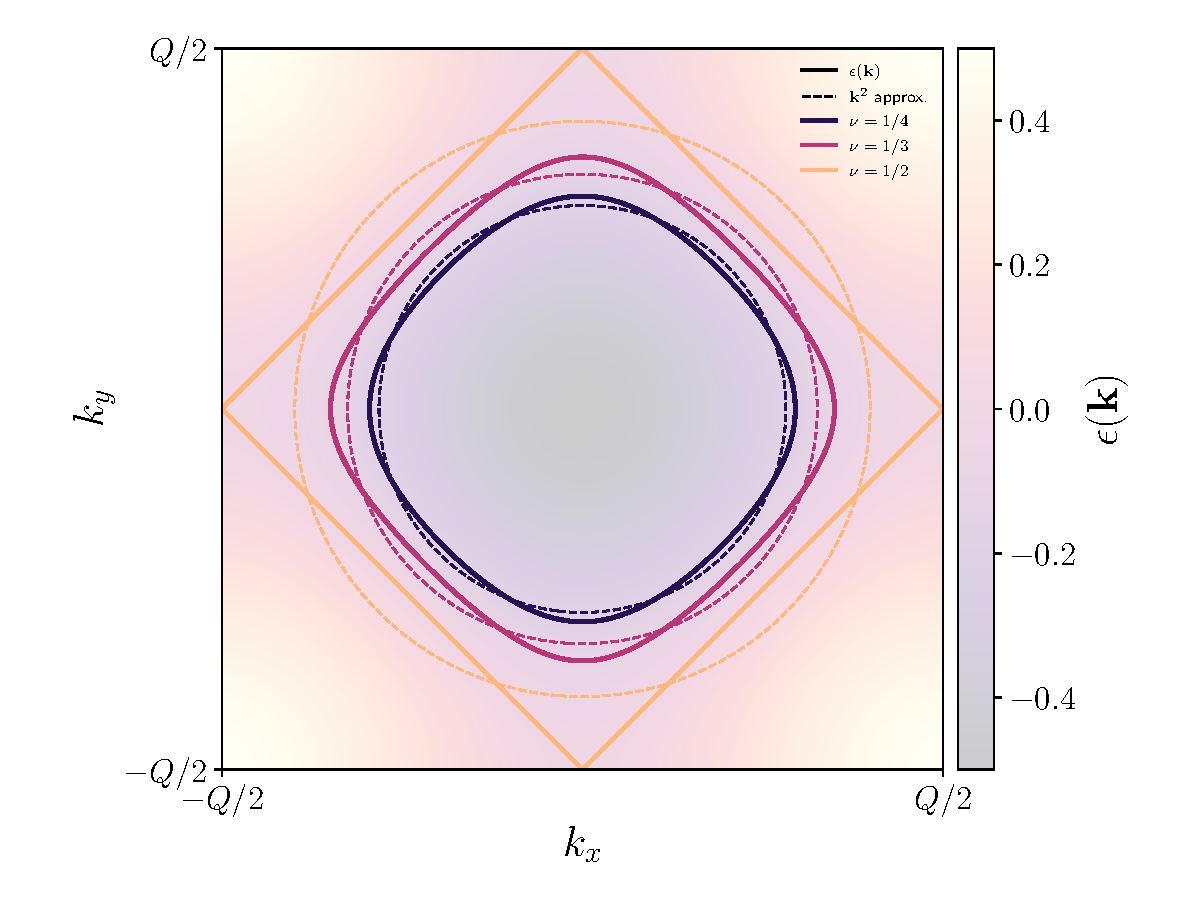
\includegraphics[width=0.6\textwidth]{plots/dispersion_with_fermi_surfaces_W_1.00.pdf}
    \caption{Dispersion $\varepsilon(\mathbf{k})$ at $W=1.0$, with the Fermi surfaces at fillings $\nu = 1/4, 1/3, 1/2$ shown both for the actual (cosine) dispersion and for a parabolic approximation.}\label{fig:fermi_surface}
\end{figure}

As shown in Fig.~\ref{fig:fermi_surface}, the Fermi surface (and even more so the density of states) of the actual dispersion differs significantly from that of the parabolic approximation, especially near the Van Hove singularity approached at $\nu = \tfrac{1}{2}$. We therefore relax this assumption: a similar criterion is derived below in which the Fermi surface is still taken to be circular for simplicity, but the density of states is obtained by numerically integrating the actual dispersion rather than assumed in a closed form.

Here $W$ is assumed to be large enough that the occupation follows a Fermi--Dirac step, $n_\tau(\mathbf{k}) = \theta(k_{F\tau}- |\mathbf{k}|)$ with $k_{F\tau}=\sqrt{2\nu_\tau}$. % chktex 8

\paragraph{Hartree energy ($\alpha=0$).} Since $\tilde U_{\tau\tau'}(0)=2\pi d_{\text{SC}}$ is independent of valley at $\alpha=0$,
\begin{equation}
    \langle \hat{H}_H \rangle = \frac{2\pi d_{\text{SC}}}{A} \sum_{\mathbf{k}, \mathbf{k'}} \sum_{\tau, \tau'} \langle n_{\mathbf{k},\tau} \rangle \langle n_{\mathbf{k'},\tau'} \rangle = \frac{2\pi d_{\text{SC}} N_{\phi}^2}{A} {(\nu_+ + \nu_-)}^2,
    \label{eq:hartree_energy_w}
\end{equation}
independent of the valley polarization.

\paragraph{Exchange energy.} At $\alpha=0$, $\tilde U_{\tau\tau}(\mathbf q) = u_0(\mathbf q)$, giving
\begin{equation}
    \langle \hat{H}_X \rangle = -\frac{1}{A} \sum_{\mathbf{q}} u_0(\mathbf{q}) e^{-q^2/2} \sum_{\tau, \mathbf{k}} n_\tau(\mathbf{k+q}) \, n_\tau(\mathbf{k}).
    \label{eq:exchange_energy_start}
\end{equation}
Converting sums to integrals ($\sum_{\mathbf{k}} \to \frac{A}{{(2\pi)}^2}\int d^2k$, and similarly for $\mathbf q$),
\begin{equation}
    E_X = -\frac{A}{{(2\pi)}^4} \int d^2q\, u_0(\mathbf{q}) e^{-q^2/2} \sum_{\tau} \int d^2k\, \theta(k_{F\tau}-|\mathbf{k+q}|)\theta(k_{F\tau}-|\mathbf{k}|).
    \label{eq:exchange_energy_integral}
\end{equation}
The inner integral is exactly the overlap area of two disks of radius $k_{F\tau}$ with centers separated by $q$,
\begin{equation}
    F(k_{F\tau}, q) = 2 k_{F\tau}^2 \arccos\!\left(\frac{q}{2 k_{F\tau}}\right) - \frac{q}{2} \sqrt{4 k_{F\tau}^2 - q^2},
    \label{eq:overlap_area}
\end{equation}
so that
\begin{equation}
    E_X = -\frac{A}{{(2\pi)}^2} \int \frac{d^2q}{{(2\pi)}^2}\, u_0(\mathbf{q}) e^{-q^2/2} \sum_\tau F(k_{F\tau}, q).
    \label{eq:exchange_energy_grouped}
\end{equation}

\paragraph{Expansion around the unpolarized point.} Write $\nu_\tau = \nu + \tau\delta$, so that $\delta$ is the polarization ($\delta=0$ corresponds to the unpolarized state), and $k_{F\tau} =\sqrt{2\nu_{\tau}}$, approximating the Fermi surface as a circle. Expanding $F$ to second order in $\delta$ and integrating over angle,
\begin{equation}
    \left. \frac{d^2 E_X}{d \delta^2} \right|_{\delta=0} = -\frac{4A}{\nu} \int_0^{\sqrt{8\nu}} \frac{q \tanh(qd_{\text{SC}})\, e^{-q^2/2}}{{(2\pi)}^2 (1+l_{\text{RK}} q)\sqrt{8\nu - q^2}}\, dq \;\equiv\; -\frac{4A}{\nu}\, \mathcal{I}_2(\nu, d_{\text{SC}}).
    \label{eq:exchange_curvature}
\end{equation}
The kinetic-energy curvature follows directly from the dispersion, obtained numerically via the density of states $D(\nu)=d\mu/d\nu$ computed from $\varepsilon_\tau(\mathbf{k})$:
\begin{equation}
    \left. \frac{d^2 E_K}{d \delta^2} \right|_{\delta=0} = 2 A W \frac{d\mu}{d\nu} = \frac{A W}{\pi} D(\nu).
    \label{eq:kinetic_curvature}
\end{equation}
The transition occurs where the curvature of the unpolarized state changes sign, i.e.\ where the kinetic cost of polarizing exactly cancels the exchange gain:
\begin{equation}
    \left. \frac{d^2 E_K}{d\delta^2} \right|_{\delta=0} + \left. \frac{d^2 E_X}{d\delta^2} \right|_{\delta=0} = 0
    \quad\Longrightarrow\quad
    \frac{AW_c}{\pi} D(\nu) = \frac{4A}{\nu}\,\mathcal{I}_2(\nu, d_{\text{SC}}),
    \label{eq:wc_condition}
\end{equation}
giving
\begin{equation}
    W_c(\nu, d_{\text{SC}}) = \frac{4\pi\, \mathcal{I}_2(\nu, d_{\text{SC}})}{\nu\, D(\nu)}.
    \label{eq:wc_formula}
\end{equation}
This result extends straightforwardly to nonzero $\alpha$ via the same procedure, giving
\begin{equation}
    W_c(\nu, d_{\text{SC}}, \alpha) = \frac{4\pi\, (1+\alpha) \mathcal{I}_2(\nu, d_{\text{SC}})}{\nu\, D(\nu)}  - \frac{4\, \alpha d_{\text{SC}}}{D(\nu)}.
    \label{eq:wc_formula_alpha}
\end{equation}

\subsection{Comparison with the numerical mean-field estimates}

We evaluate the analytic estimates of Secs.~\ref{subsec:alpha_transition}--\ref{subsec:w_transition} numerically at the default parameters $d_{\text{SC}}=6a$, $l_{\text{RK}}=0$, using $D(\nu)$ obtained from the actual cosine dispersion (Fig.~\ref{fig:fermi_surface}) rather than the parabolic approximation, and compare against the ED phase diagrams below.

At $W=0$, Eqs.~\eqref{eq:alpha_c_case1}--\eqref{eq:alpha_c_case2} give $\alpha_c \approx 0.042$ at $\nu=\frac13$ per valley, compared to the ED value $\alpha_c \approx 0.004$ extracted from Fig.~\ref{fig:third_third_phase_diagram}. The mean-field estimate thus overestimates $\alpha_c$ by roughly an order of magnitude, but correctly predicts the direction of the polarized phase ($\alpha < \alpha_c$ in the $U(\mathbf{q}=0)\neq 0$ case), proximity to the valley-isotropic point and, more importantly, its trend: scanning $\alpha_c(d_{\text{SC}})$ and $\alpha_c(l_{\text{RK}})$ analytically gives a monotonic decrease with both parameters, matching the monotonic narrowing of the $\alpha$-stable FQH region with increasing $d_{\text{SC}}$ and $l_{\text{RK}}$ observed in Figs.~\ref{fig:third_third_screening_alpha_vs_d_phase_diagram_a} and~\ref{fig:third_third_screening_alpha_vs_lRK_phase_diagram_b}.


For the $W$-driven depolarization transition, the mean-field estimate at $\nu = \tfrac13$, $\alpha = 0$ gives $W_c \approx 0.84$, compared to the ED result of $W \sim 0.5$ read off from Fig.~\ref{fig:third_third_phase_diagram}. As with $\alpha_c$, the analytic estimate is systematically too large but of the correct order of magnitude, consistent with the general tendency of Hartree-Fock to overestimate the stability of ordered phases by neglecting quantum fluctuations.


Overall, the analytic mean-field treatment reproduces the correct qualitative structure of the phase diagram --- the existence and approximate location of both the $\alpha$- and $W$-driven depolarization transitions, and their correct monotonic dependence on the screening parameters $d_{\text{SC}}$ and $l_{\text{RK}}$ --- while systematically overestimating both $\alpha_c$ and $W_c$.

\section{\texorpdfstring{Phase diagram for $\nu = \frac{2}{3}$}{Phase diagram for nu = 2/3}}\label{sec:third_third_results}

At this filling, an FQH state is expected at $W=0$ in the valley-polarized region, and an FTI state at $\alpha=1$, $W=0$. We now present the numerical phase diagram, addressing how resilient these topological phases are against nonzero $|W|$ and non-ideal $\alpha$, and examine phase transitions found in the system, and the dependence of stability of topological phases on the screening parameters $d_{\text{SC}}$ and $l_{\text{RK}}$.

\begin{figure}[htbp]
    \centering
    \begin{subfigure}{0.45\textwidth}
        \centering
        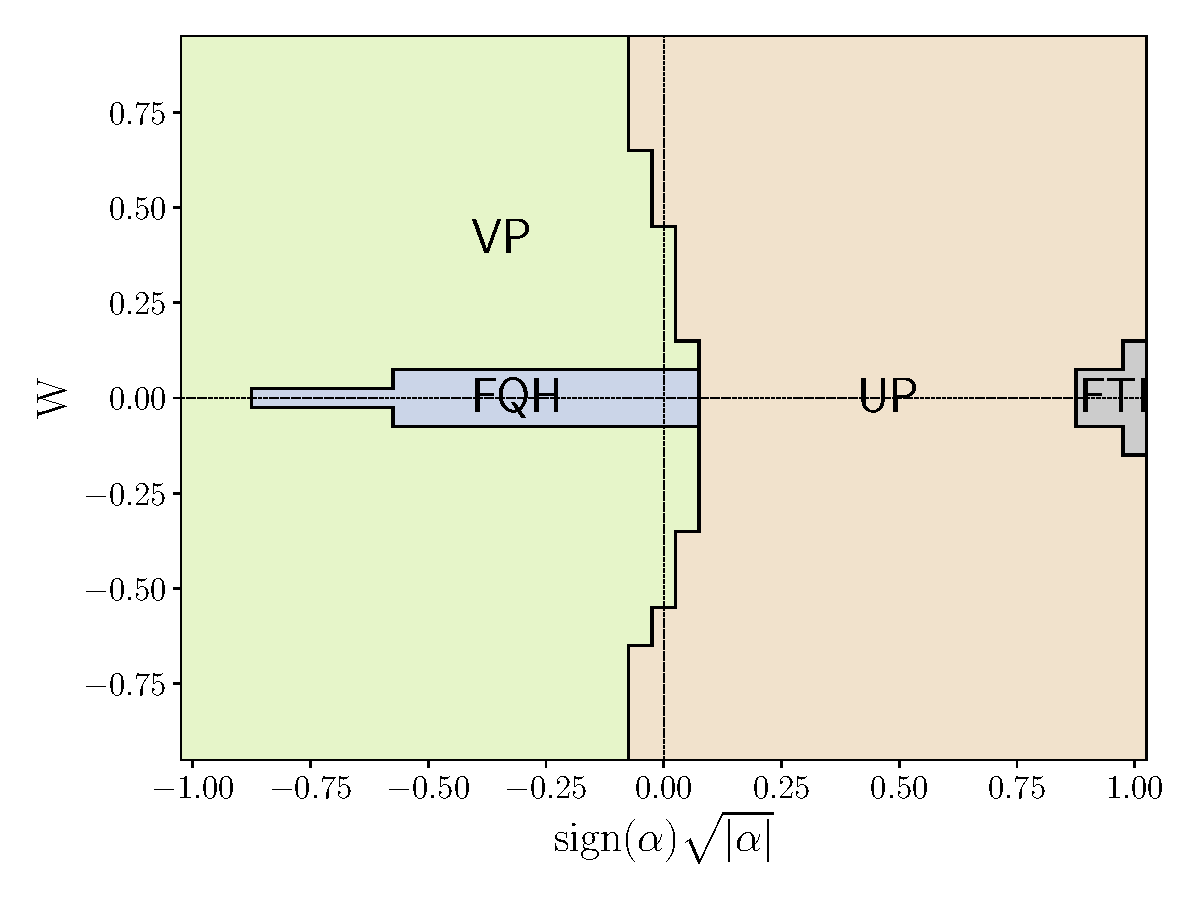
\includegraphics[width=1.0\textwidth]{plots/third_third_phase_diagram.pdf}
        \subcaption{$U(\mathbf{q}=0) \neq 0$}\label{fig:third_third_phase_diagram}
    \end{subfigure}
    \begin{subfigure}{0.45\textwidth}
        \centering
        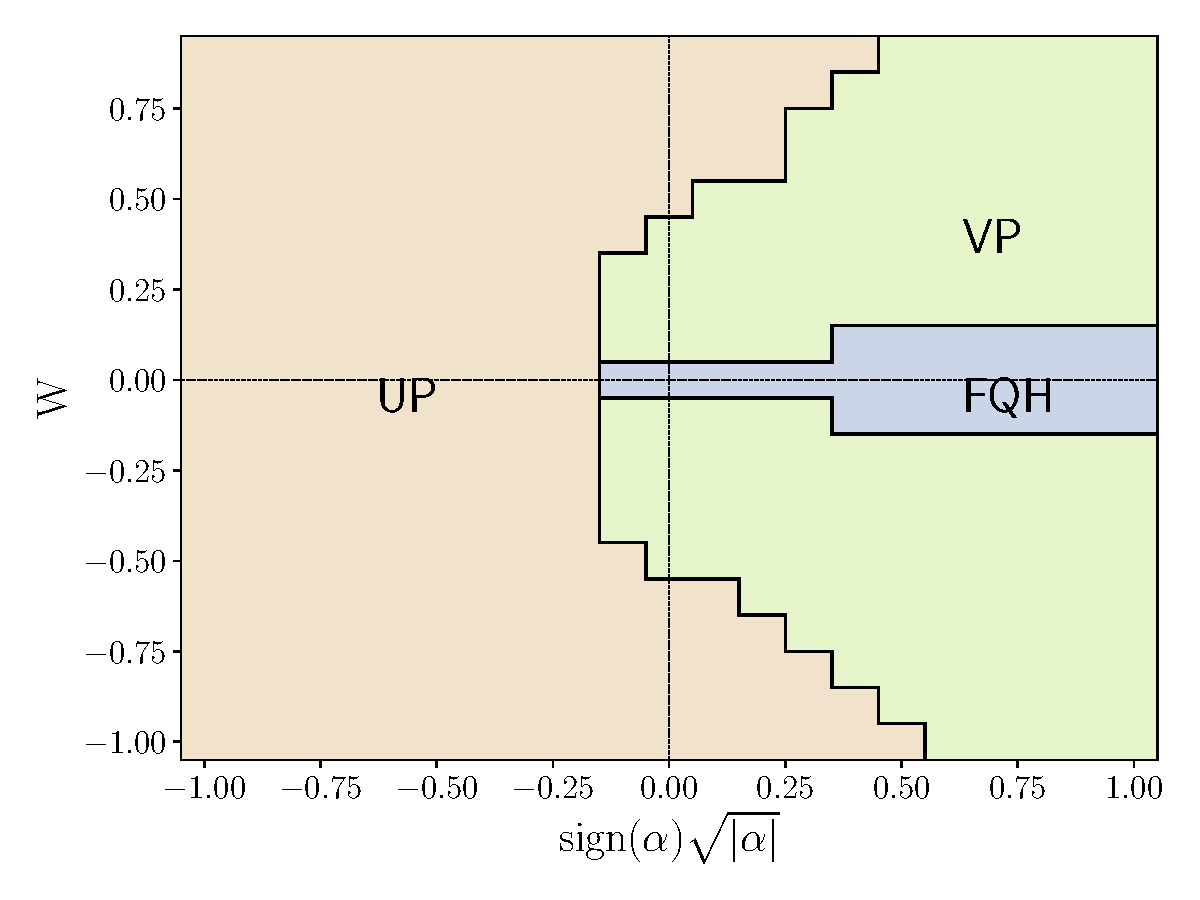
\includegraphics[width=1.0\textwidth]{plots/third_third_q0_phase_diagram.pdf}
        \subcaption{$U(\mathbf{q}=0) = 0$}\label{fig:third_third_q0_phase_diagram}
    \end{subfigure}
    \begin{subfigure}{0.45\textwidth}
        \centering
        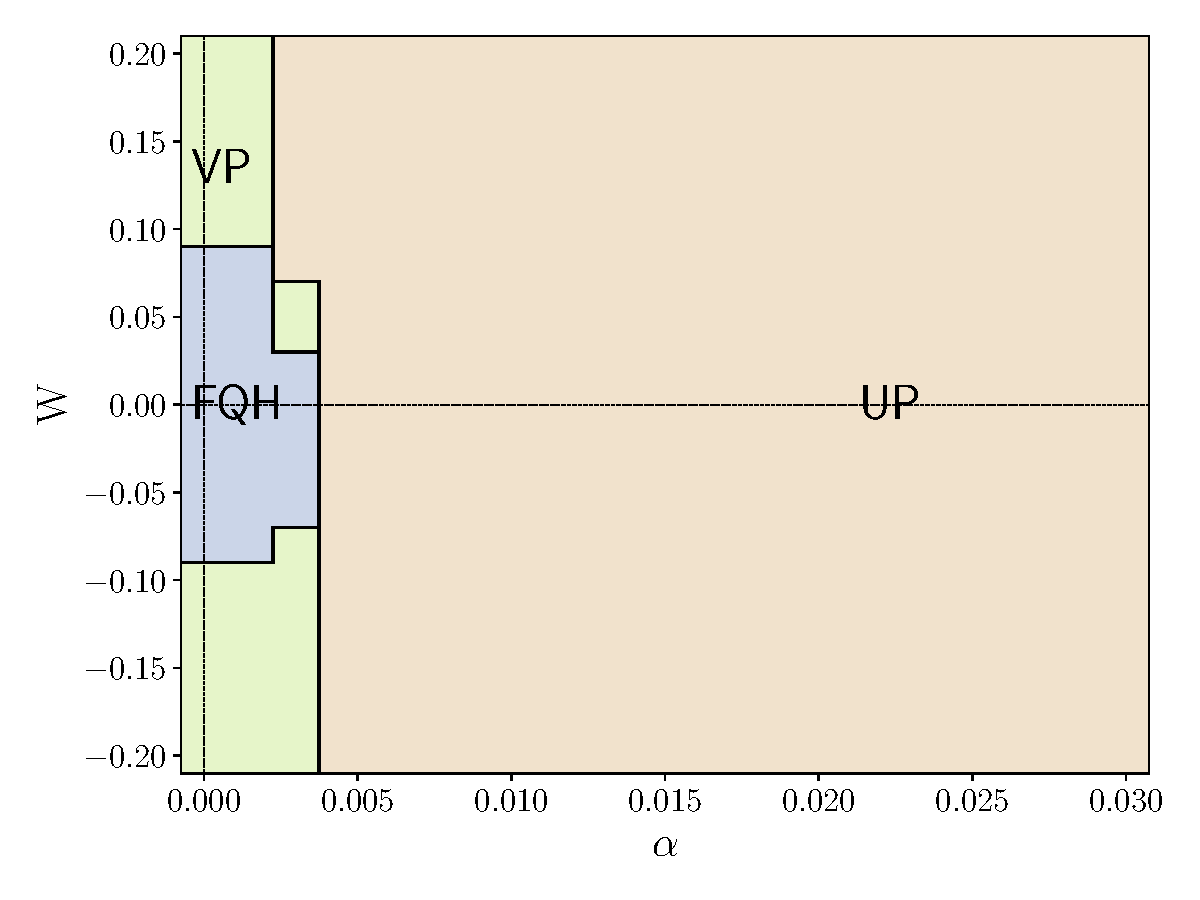
\includegraphics[width=1.0\textwidth]{plots/third_third_zoom_3_phase_diagram.pdf}
        \subcaption{Zoom-in on the FQH ($U(\mathbf{q}=0) \neq 0$)}\label{fig:third_third_zoom_3_phase_diagram}
    \end{subfigure}
    \begin{subfigure}{0.45\textwidth}
        \centering
        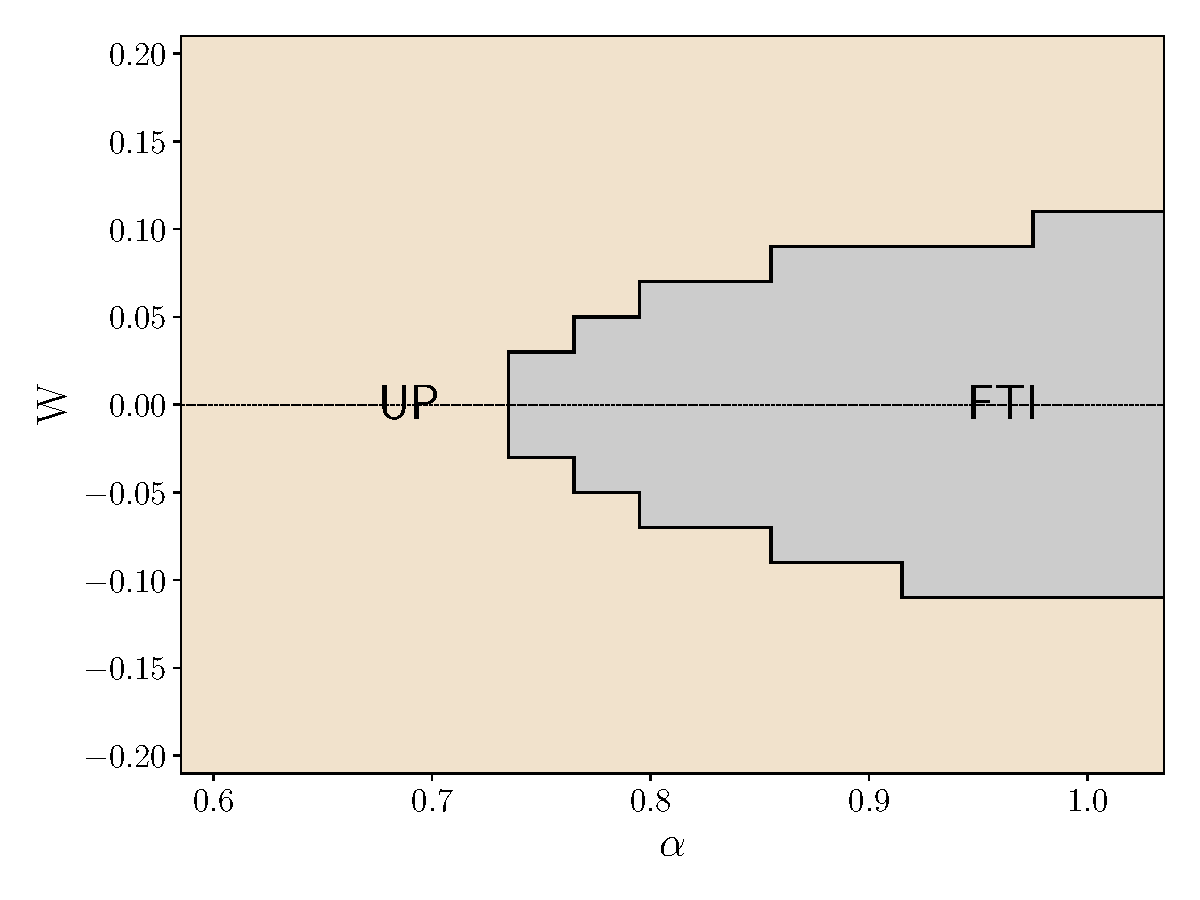
\includegraphics[width=1.0\textwidth]{plots/third_third_zoom_9_phase_diagram.pdf}
        \subcaption{Zoom-in on the FTI ($U(\mathbf{q}=0) \neq 0$)}\label{fig:third_third_zoom_9_phase_diagram}
    \end{subfigure}
    \caption{Phase diagrams of the $\nu = \frac{2}{3}$ filling. VP:\@ gapless valley-polarized state. UP:\@ general unpolarized state. FQH:\@ 3-fold degenerate valley-polarized fractional quantum Hall state. FTI:\@ 9-fold degenerate valley-unpolarized fractional topological insulator. See Fig.~\ref{fig:summary} for a schematic identification of the UP regions.}\label{fig:third_third_phases}
\end{figure}

Figure~\ref{fig:third_third_phases} presents the phase diagram at $\nu=\frac{2}{3}$. The only significant gaps found in the system are $\Delta_3$, $\Delta_6$ (discussed below) and $\Delta_9$. In the $U(\mathbf{q}=0) \neq 0$ case (Fig.~\ref{fig:third_third_phase_diagram}), full valley polarization is observed at low $|W|$ and low $\alpha$, with $\alpha_c \approx 0.004$, while the unpolarized state prevails at larger $\alpha$. At $\alpha=1$, down to $\alpha \approx 0.72$, the unpolarized state shows a clear 9-fold degeneracy, consistent with the FTI state (each FQH copy contributing a 3-fold degeneracy). The valley-polarized region itself splits into two parts. At low $|W|$ the state has a topological 3-fold degeneracy, consistent with a $\nu=\frac{2}{3}$ FQH state in a single valley. The topological nature of FQH and FTI phases is confirmed below via spectral flow. Both of them survive a nonzero bandwidth, up to $|W| \approx 0.09$ for the FQH state and $|W| \approx 0.1$ for the FTI state. The similarity of these two values is consistent with the ideal FQH and FTI states incurring the same kinetic energy penalty from $W$. At intermediate $|W|$, the FQH state transitions into a gapless valley-polarized state (denoted as VP) --- driven by the kinetic-energy cost of the flat momentum occupation characteristic of the FQH state --- and, at an $\alpha$-dependent $W_c$ on the order of $\pm0.5$, into a valley-unpolarized state. The FTI state undergoes an analogous transition into a gapless state at increasing $W$.

The phase diagram is approximately symmetric about the $W=0$ axis, as suspected from the analysis in \S\ref{sec:symmetries}. The symmetry being only approximate is a finite size effect, in particular related to the fact that the sampling of the Brillouin zone is not invariant under the $\pm \mathbf{Q_0}$ shift. At $\alpha \to -1$, the FQH state is not detected, since valley polarization combined with the vanishing intra-valley interaction renders the system effectively noninteracting, closing the spectral gap.

A different picture emerges for the $U(\mathbf{q}=0) = 0$ phase diagram (Fig.~\ref{fig:third_third_q0_phase_diagram}), where the valley-polarized region instead occupies large $\alpha$, and the unpolarized --- small $\alpha$. The same VP and FQH phases appear, with a similar $W$-dependent transition between them, but because the polarized phase now extends across the entire $\alpha > 0$ region, no FTI state is found. At low $\alpha$, only a non-polarized gapless state is found --- it is not investigated further.

\subsection{\texorpdfstring{Phase transitions at $W\approx0$ and variable $\alpha$}{Phase transitions at W approx 0 and variable alpha}}

\begin{figure}[htbp]
    \centering
    \begin{subfigure}{0.3\textwidth}
        \centering
        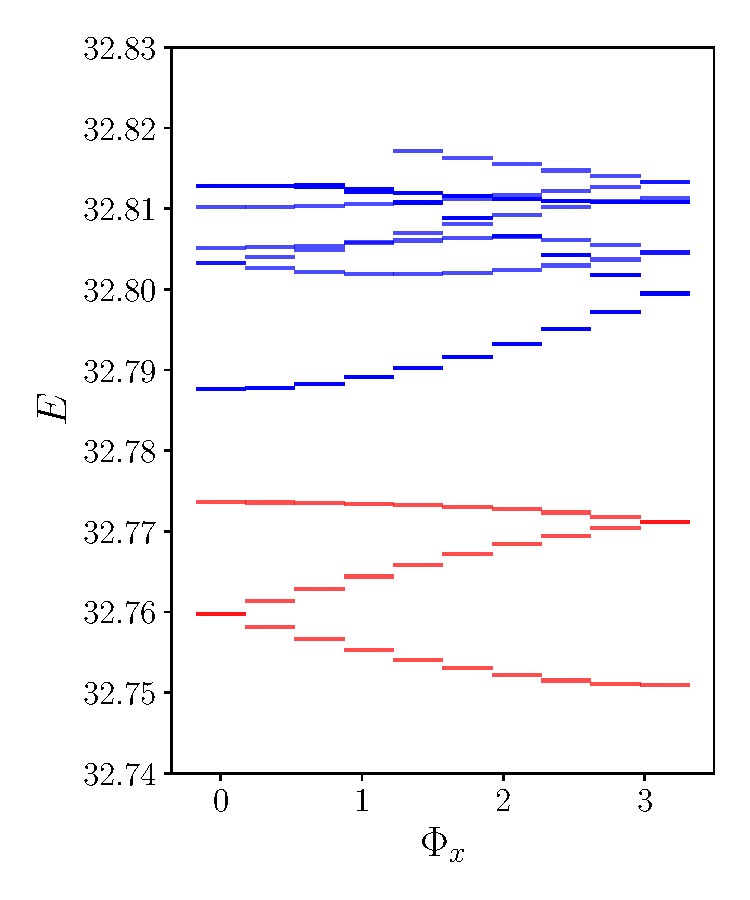
\includegraphics[width=1.0\textwidth]{plots/alpha_transition_W=0.05_alpha=0.0024.pdf}
        \subcaption{$\alpha = 0.0024$ --- FQH}\label{fig:low_alpha_transition_a}
    \end{subfigure}
    \begin{subfigure}{0.3\textwidth}
        \centering
        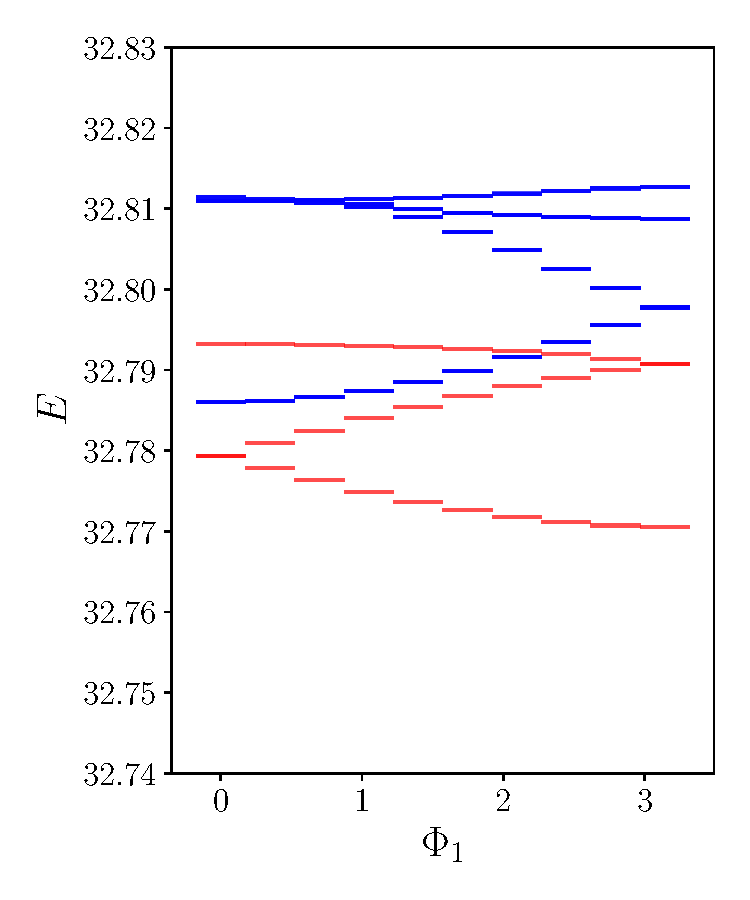
\includegraphics[width=1.0\textwidth]{plots/alpha_transition_W=0.05_alpha=0.003.pdf}
        \subcaption{$\alpha = 0.003$ --- gapless}\label{fig:low_alpha_transition_b}
    \end{subfigure}
    \begin{subfigure}{0.3\textwidth}
        \centering
        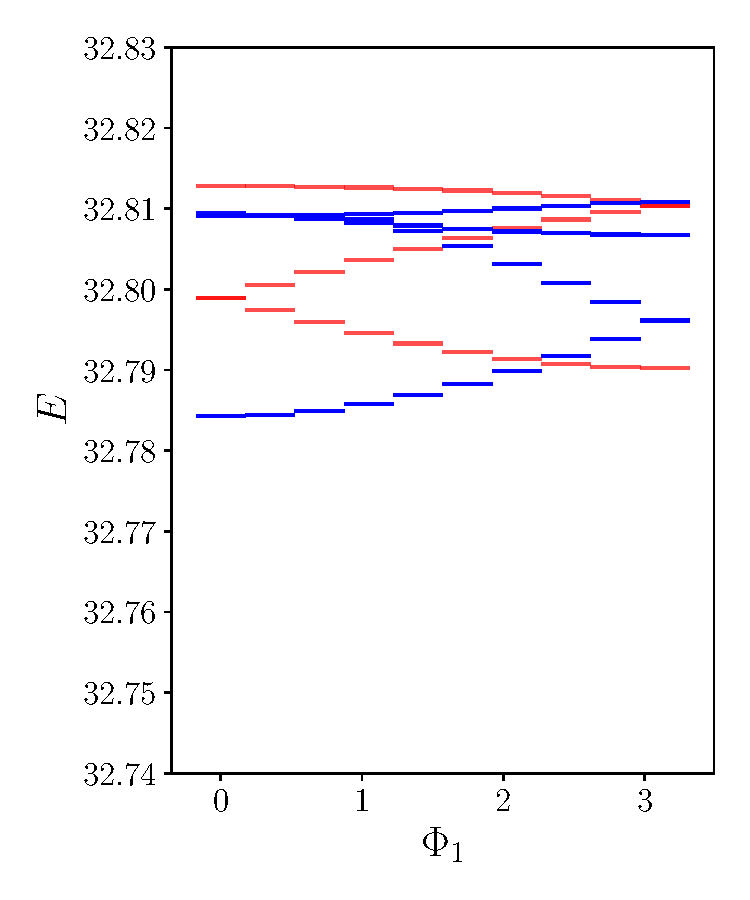
\includegraphics[width=1.0\textwidth]{plots/alpha_transition_W=0.05_alpha=0.0036.pdf}
        \subcaption{$\alpha = 0.0036$ --- gapless}\label{fig:low_alpha_transition_c}
    \end{subfigure}
    \caption{Flux insertion plots of the energy spectrum near the valley-isotropic limit $\alpha\approx 0$, at $W=0.05$ and $\nu = \frac{2}{3}$, showing the transition from the FQH state to a gapless state. Ground-state manifold shown in red.}\label{fig:low_alpha_transition}
\end{figure}

The nature of the phase transition out of the FQH state is illustrated in Figure~\ref{fig:low_alpha_transition}, which shows the energy spectrum under flux insertion at $W=0.05$ for different $\alpha$ values, across the transition out of the FQH phase. Interestingly, the 3-fold degenerate ground-state manifold survives the transition; the only change is the relative energy of the manifold with respect to the gapless continuum above it.

\begin{figure}[htbp]
    \centering
    \begin{subfigure}{0.3\textwidth}
        \centering
        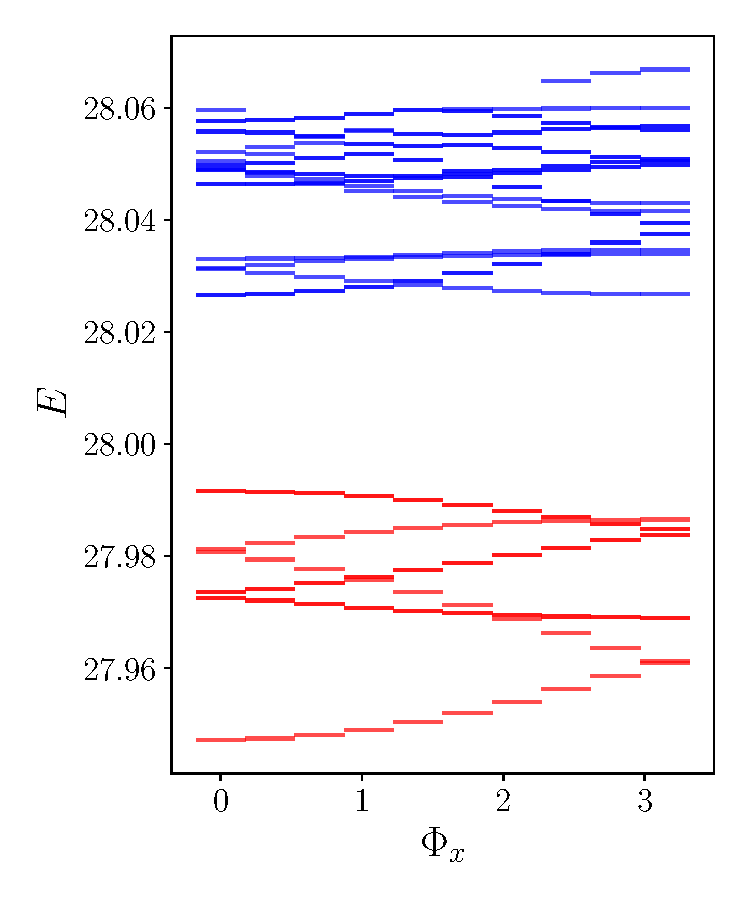
\includegraphics[width=1.0\textwidth]{plots/alpha1_transition_W=0.05_alpha=0.8500000000000001.pdf}
        \subcaption{$\alpha = 0.85$ --- FTI state}\label{fig:high_alpha_transition_a}
    \end{subfigure}
    \begin{subfigure}{0.3\textwidth}
        \centering
        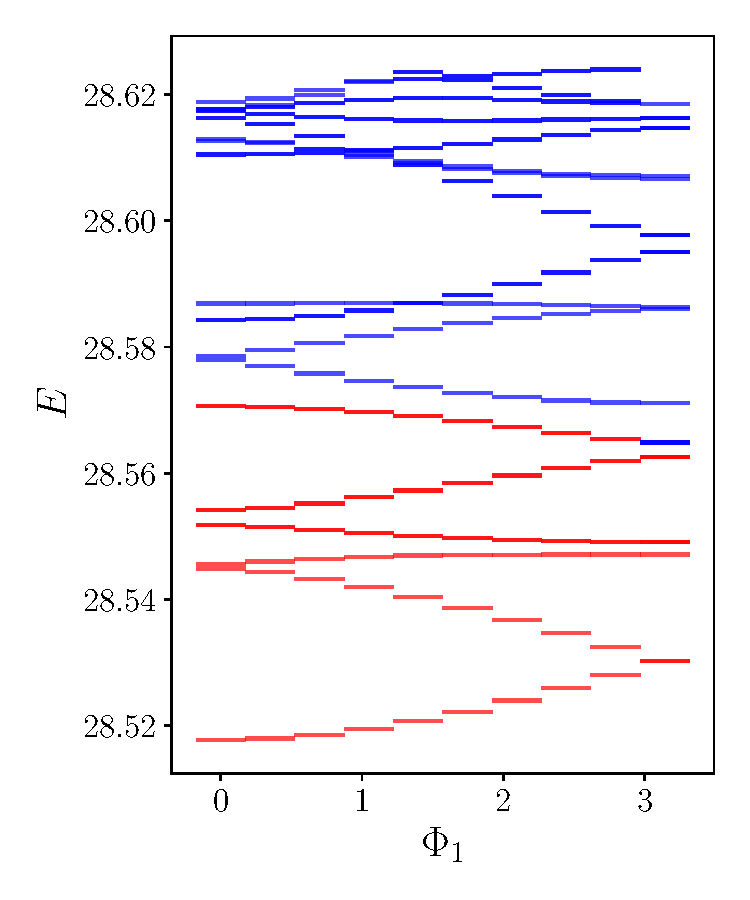
\includegraphics[width=1.0\textwidth]{plots/alpha1_transition_W=0.05_alpha=0.76.pdf}
        \subcaption{$\alpha = 0.76$ --- gapless state}\label{fig:high_alpha_transition_b}
    \end{subfigure}
    \caption{Phase winding of the energy spectrum near the decoupled limit $\alpha \approx 1$, at $W=0.05$ and $\nu = \frac{2}{3}$, showing the transition from the FTI state to a gapless state. Ground-state manifold shown in red.}\label{fig:high_alpha_transition}
\end{figure}

Figure~\ref{fig:high_alpha_transition} shows the analogous phase winding at $W=0.05$ with $\alpha$ decreasing from the FTI-like state. As before, the ground-state manifold moves relative to the excited-state continuum until the 9-fold degenerate gap closes. However, the relative energy splitting between the lowest 3 states of the ground-state manifold and the remaining 6 grows on approach to the transition, eventually opening a gap between them: a nonzero 3-fold gap in the otherwise unpolarized state is indeed found in a small region of the phase diagram. As described below (\S\ref{sec:third_third_density}), this phase is not topological.

\subsection{\texorpdfstring{Spectral flow \& phase transitions with variable $W$}{Phase transitions with variable W}}

\begin{figure}[htbp]
    \centering
    \begin{subfigure}{0.3\textwidth}
        \centering
        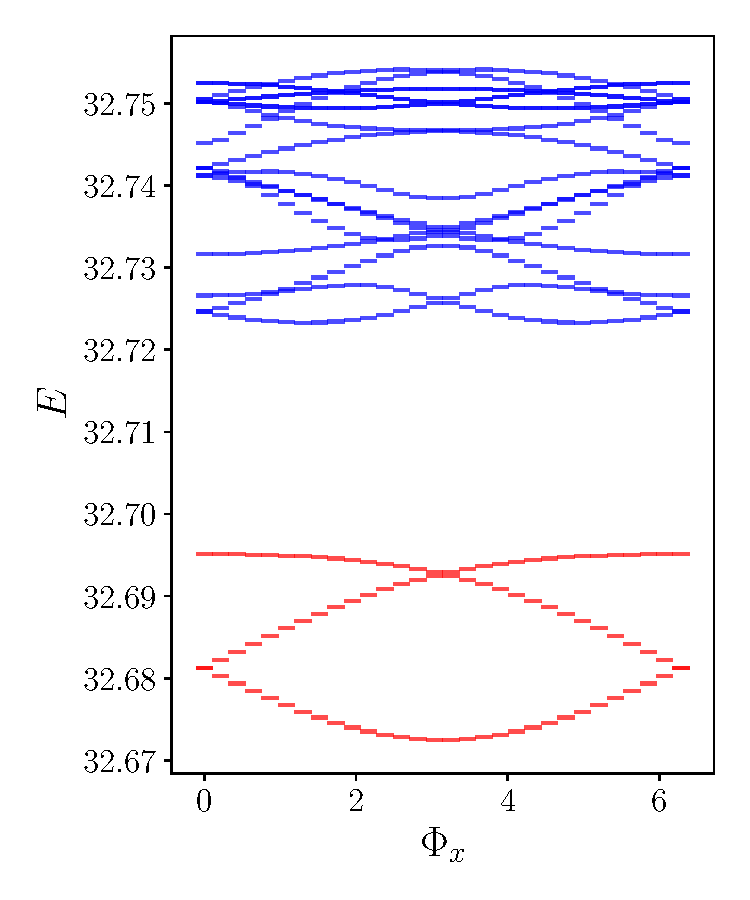
\includegraphics[width=1.0\textwidth]{plots/phase_winding_W=0.05_alpha=0.0.pdf}
        \subcaption{$W=0.05$}\label{fig:phase_winding_low_alpha_a}
    \end{subfigure}
    \begin{subfigure}{0.3\textwidth}
        \centering
        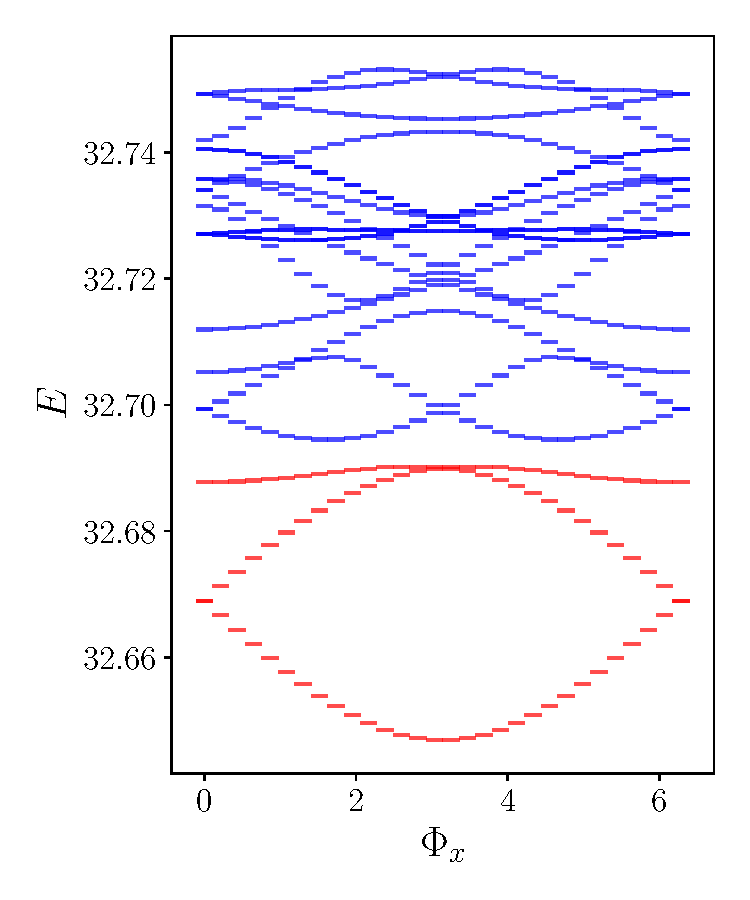
\includegraphics[width=1.0\textwidth]{plots/phase_winding_W=0.1_alpha=0.0.pdf}
        \subcaption{$W=0.1$}\label{fig:phase_winding_low_alpha_b}
    \end{subfigure}
    \begin{subfigure}{0.3\textwidth}
        \centering
        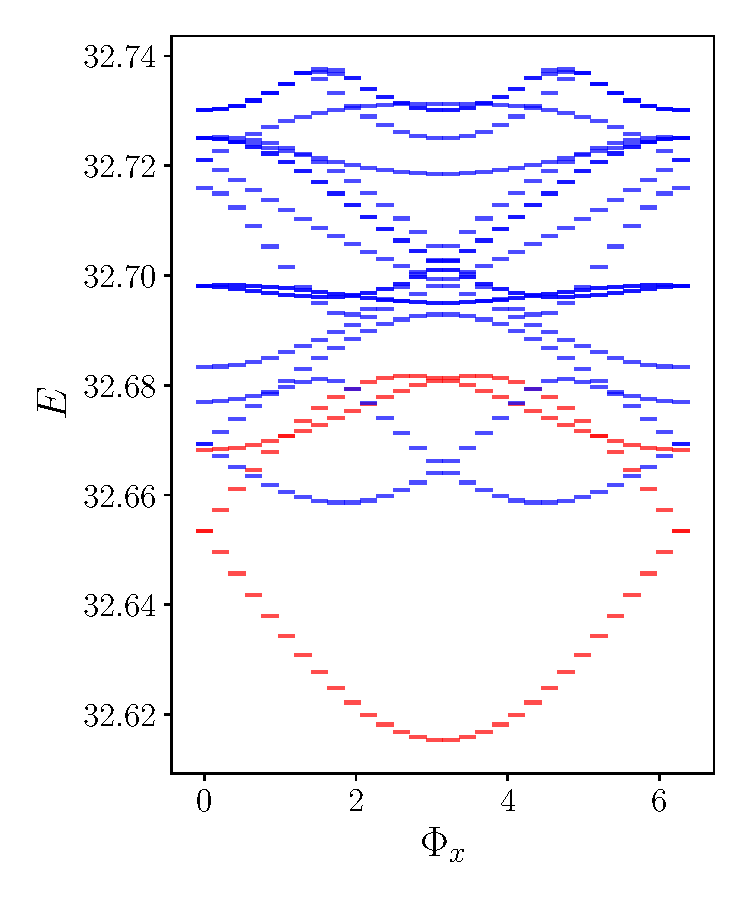
\includegraphics[width=1.0\textwidth]{plots/phase_winding_W=0.15_alpha=0.0.pdf}
        \subcaption{$W=0.15$}\label{fig:phase_winding_low_alpha_c}
    \end{subfigure}
    \caption{Phase winding of the energy spectrum at $\alpha=0$ and $\nu = \frac{2}{3}$, showing the transition from the FQH state to a gapless state with increasing $W$. Ground-state manifold shown in red.}\label{fig:phase_winding_low_alpha}
\end{figure}

\begin{figure}[htbp]
    \centering
    \begin{subfigure}{0.3\textwidth}
        \centering
        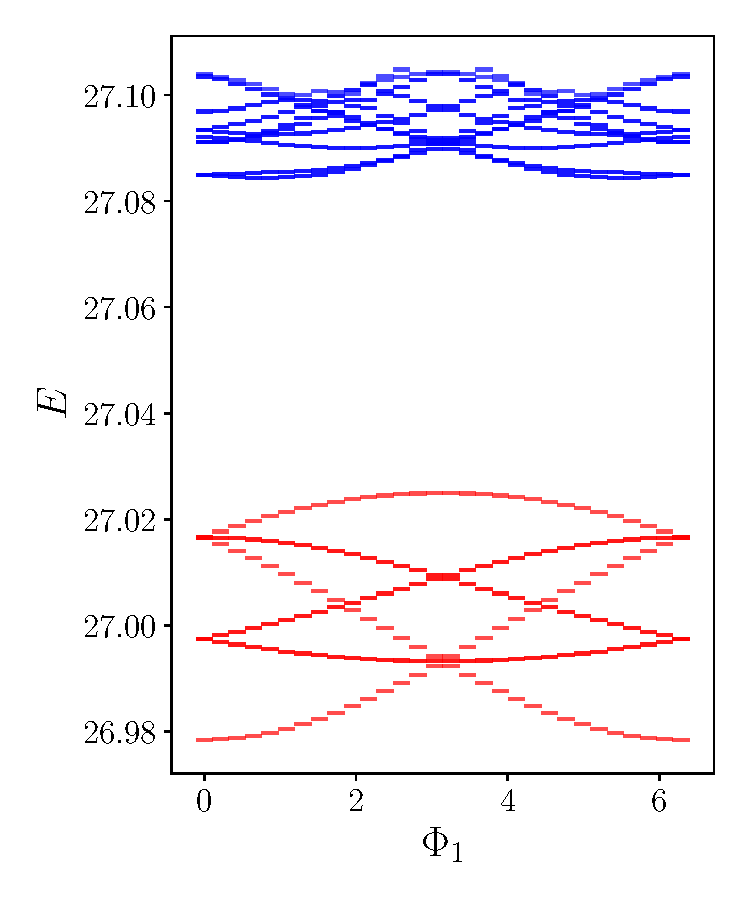
\includegraphics[width=1.0\textwidth]{plots/phase_winding_W=0.05_alpha=1.0.pdf}
        \subcaption{$W=0.05$}\label{fig:phase_winding_high_alpha_a}
    \end{subfigure}
    \begin{subfigure}{0.3\textwidth}
        \centering
        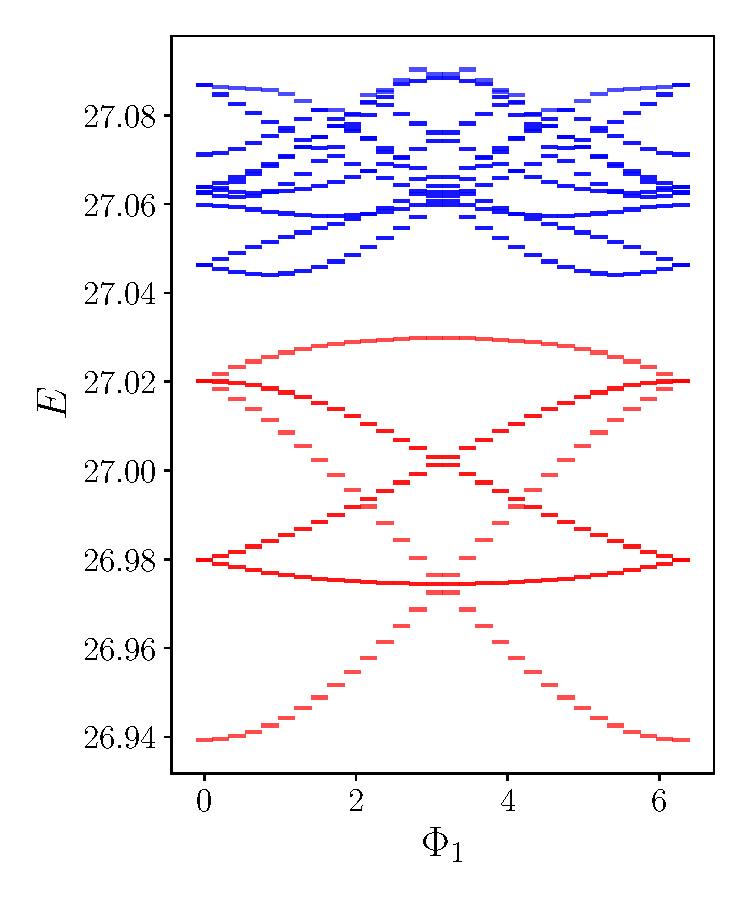
\includegraphics[width=1.0\textwidth]{plots/phase_winding_W=0.1_alpha=1.0.pdf}
        \subcaption{$W=0.1$}\label{fig:phase_winding_high_alpha_b}
    \end{subfigure}
    \begin{subfigure}{0.3\textwidth}
        \centering
        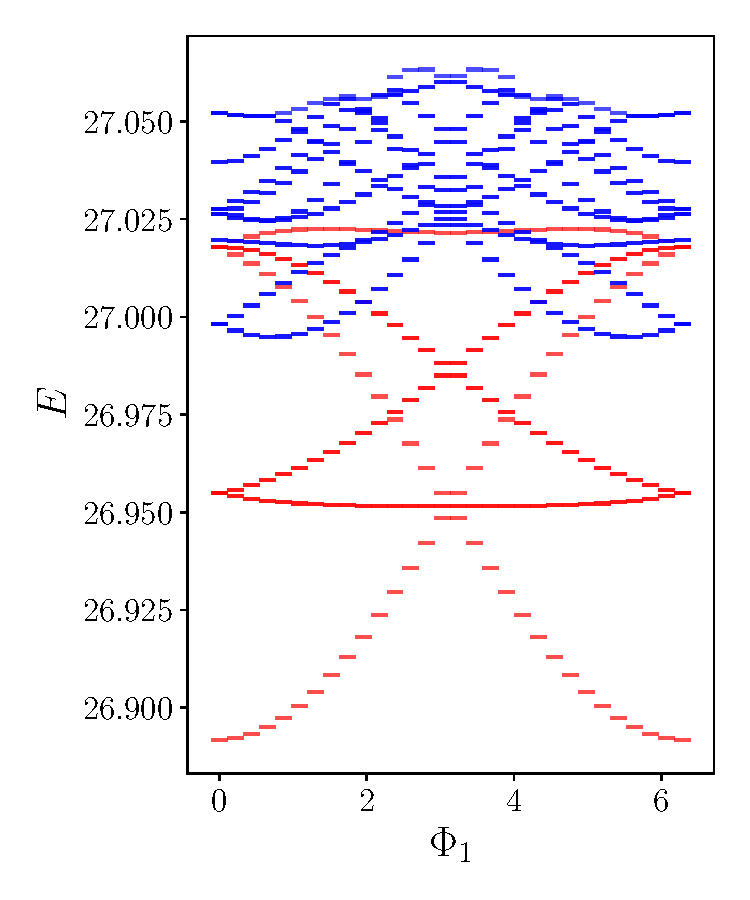
\includegraphics[width=1.0\textwidth]{plots/phase_winding_W=0.15_alpha=1.0.pdf}
        \subcaption{$W=0.15$}\label{fig:phase_winding_high_alpha_c}
    \end{subfigure}
    \caption{Phase winding of the energy spectrum at $\alpha=1$ and $\nu = \frac{2}{3}$, showing the transition from the FTI state to a gapless state with increasing $W$. Ground-state manifold shown in red.}\label{fig:phase_winding_high_alpha}
\end{figure}

Figures~\ref{fig:phase_winding_low_alpha} and~\ref{fig:phase_winding_high_alpha} show the energy spectrum for the FQH ($\alpha=0.0$) and FTI ($\alpha=1$) phases respectively, under flux insertion. At low $W$ (Figs.~\ref{fig:phase_winding_low_alpha_a} and~\ref{fig:phase_winding_high_alpha_a}), spectral flow of the ground-state manifold is directly observed: the spectrum at $\Phi_1 = 0$ and $\Phi_1 = 2\pi$ is identical, but the states within the manifold are cyclically permuted, returning to their original positions only after $\Phi_1 = 6\pi$. This further confirms the topological nature of both phases. The remaining panels of each figure visualize the transition from the topological to the gapless phase as the increasing bandwidth closes the spectral gap.

\subsection{\texorpdfstring{Nature of the intermediate--$\alpha$ and high-$|W|$ phases}{Nature of the intermediate-alpha and high-W phases}}\label{sec:third_third_density}

\begin{figure}[htbp]
    \centering
    \begin{subfigure}{0.45\textwidth}
        \centering
        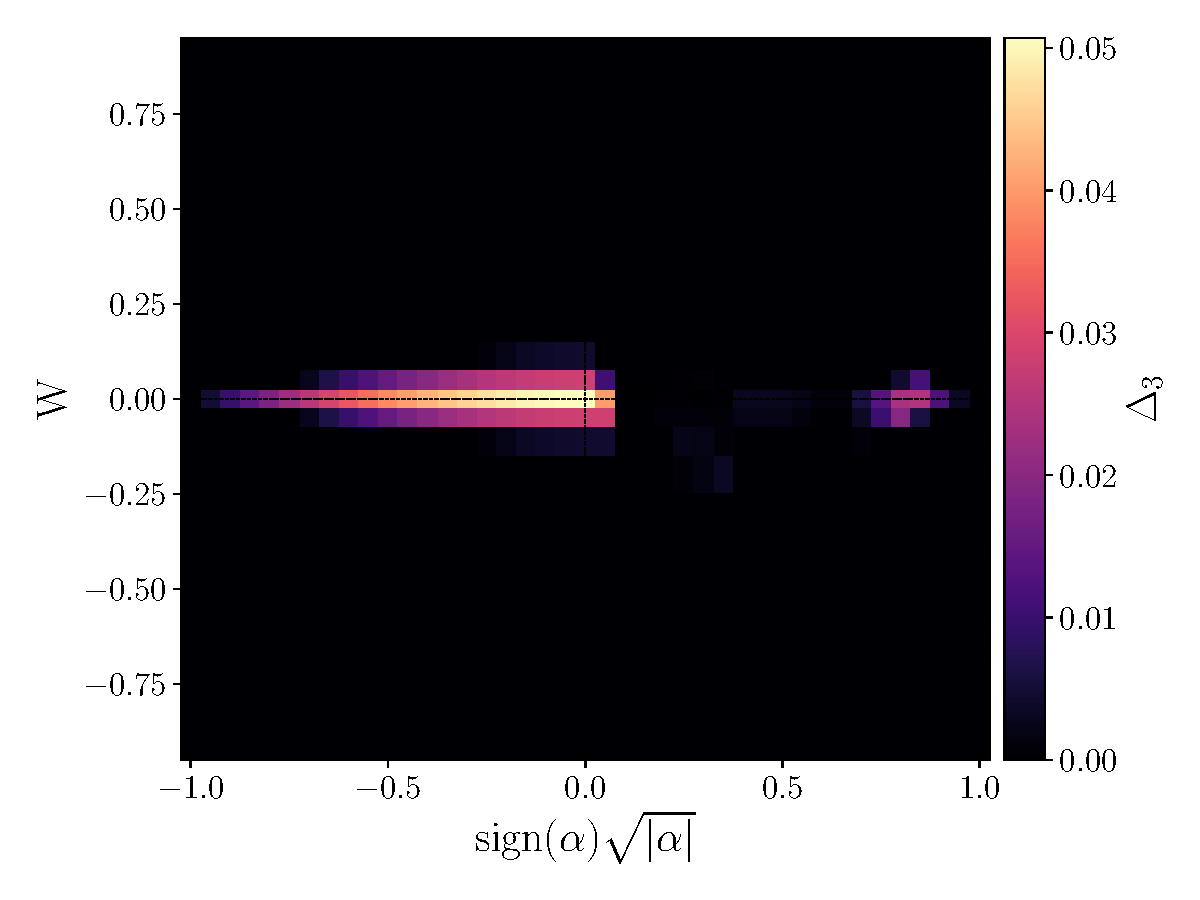
\includegraphics[width=1.0\textwidth]{plots/third_third_gap_n3.pdf}
        \subcaption{$\Delta_3$}\label{fig:third_third_gap_n3}
    \end{subfigure}
    \begin{subfigure}{0.45\textwidth}
        \centering
        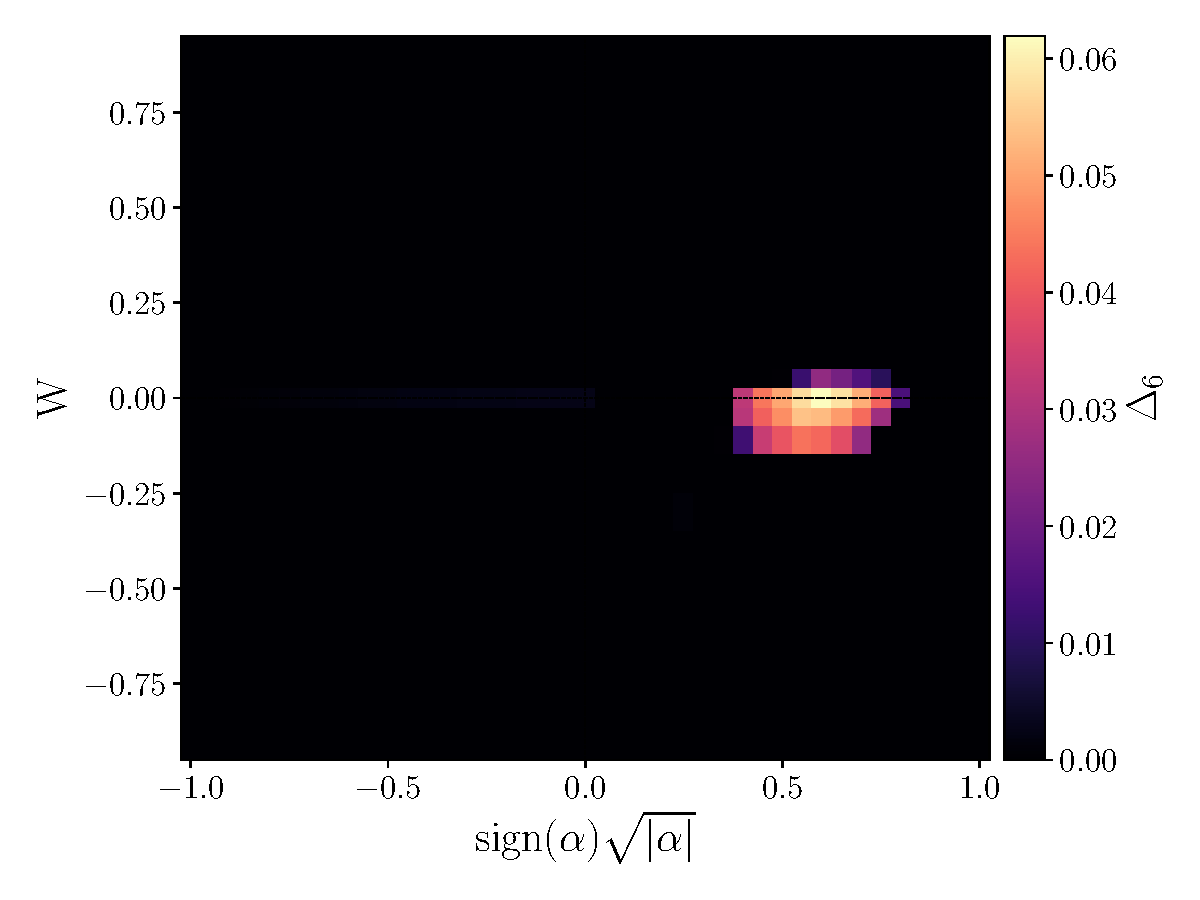
\includegraphics[width=1.0\textwidth]{plots/third_third_gap_n6.pdf}
        \subcaption{$\Delta_6$}\label{fig:third_third_gap_n6}
    \end{subfigure}
    \begin{subfigure}{0.45\textwidth}
        \centering
        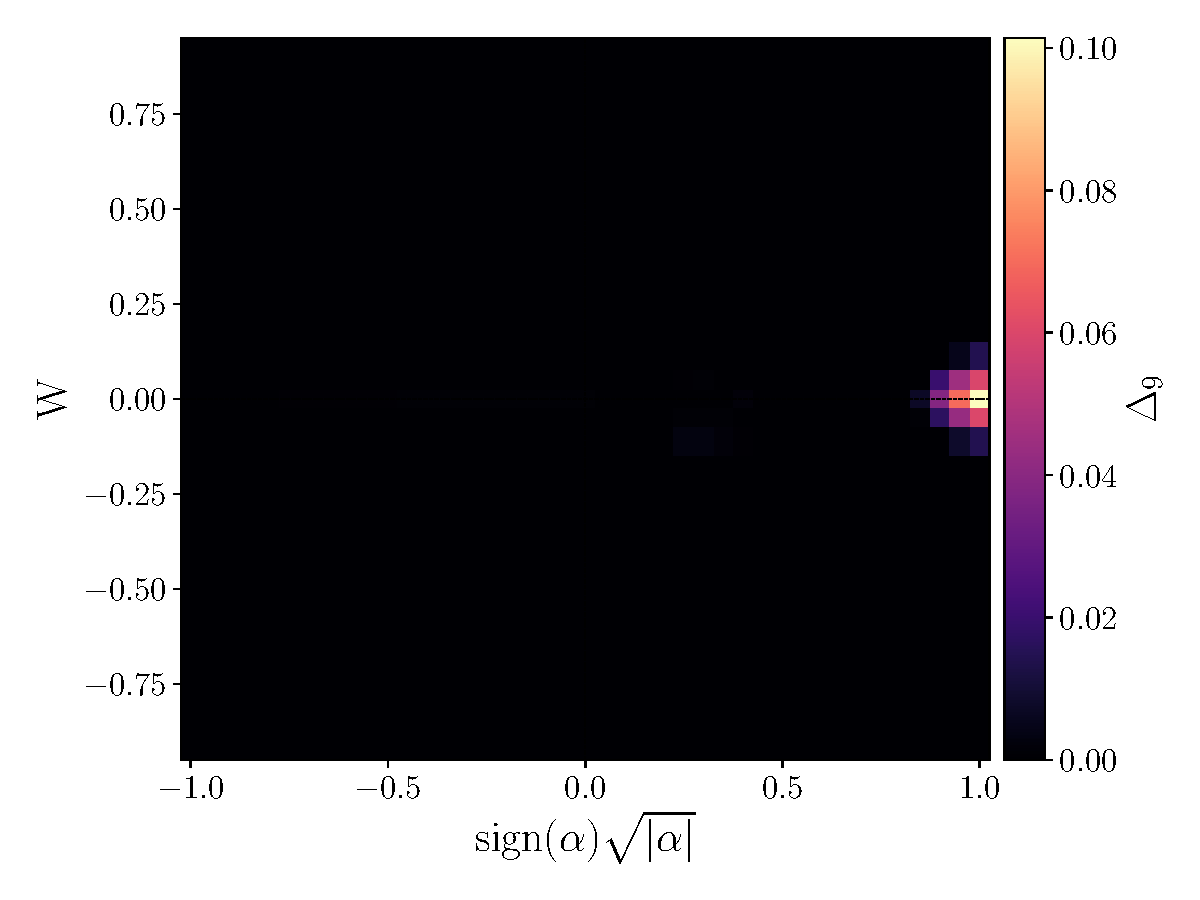
\includegraphics[width=1.0\textwidth]{plots/third_third_gap_n9.pdf}
        \subcaption{$\Delta_9$}\label{fig:third_third_gap_n9}
    \end{subfigure}
    \begin{subfigure}{0.25\textwidth}
        \centering
        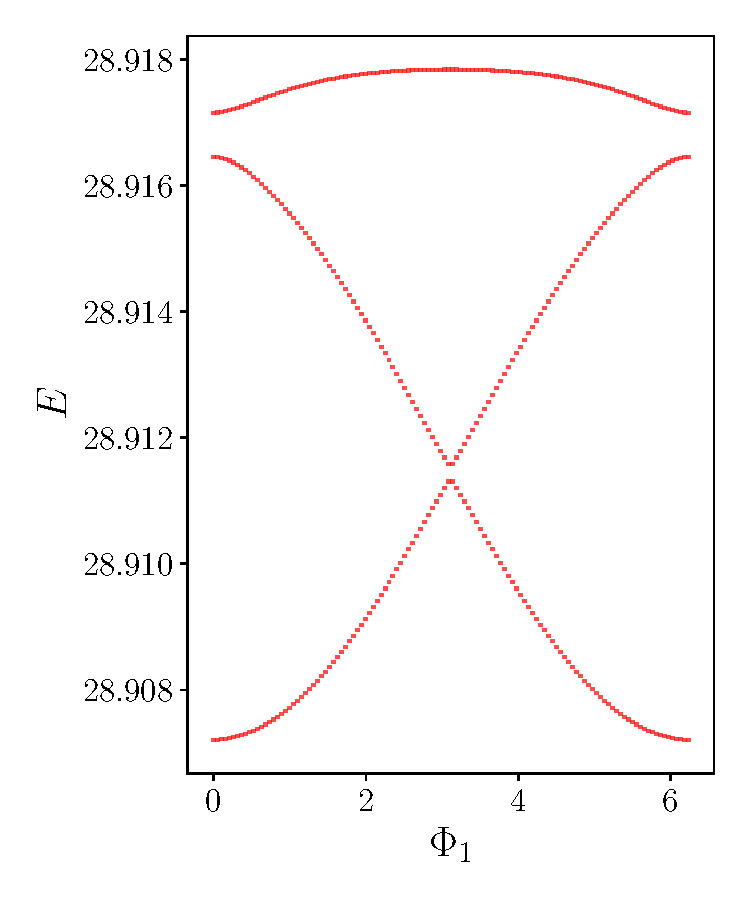
\includegraphics[width=1.0\textwidth]{plots/phase_winding_halperin_W=0.025_alpha=0.7.pdf}
        \subcaption{$\alpha=0.7$, $W=0.025$}\label{fig:phase_winding_3fold_degenerate}
    \end{subfigure}
    \begin{subfigure}{0.25\textwidth}
        \centering
        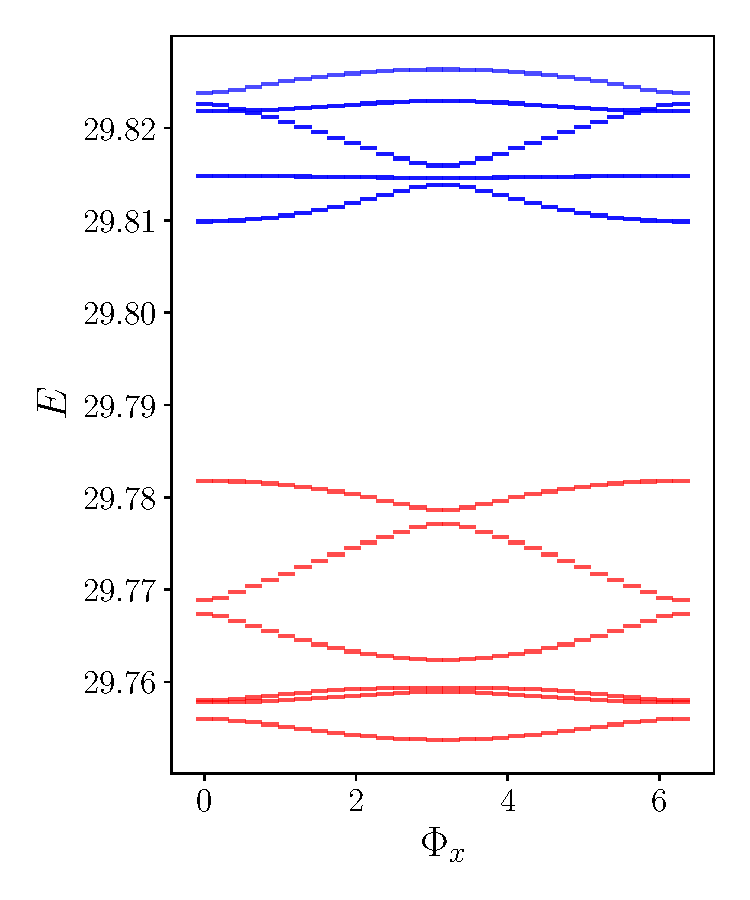
\includegraphics[width=1.0\textwidth]{plots/phase_winding_W=0.025_alpha=0.5625.pdf}
        \subcaption{$\alpha=0.56$, $W=0.025$}\label{fig:phase_winding_6fold_degenerate}
    \end{subfigure}
    \caption{(a-c) Spectral gaps in the system as a function of $\alpha$ and $W$, at $\nu=\frac{2}{3}$. (d-e) Flux insertion of the 3-fold and 6-fold degenerate states, respectively.}\label{fig:third_third_gaps}
\end{figure}

Figure~\ref{fig:third_third_gaps} shows the size of the $\Delta_3$, $\Delta_6$, and $\Delta_9$ gaps across the phase diagram. It confirms directly that the FQH and FTI states are most stable at $W=0$, where the corresponding gap is largest. Notably, non-zero $\Delta_3$ and $\Delta_6$ gaps are also found in the unpolarized phase at intermediate $\alpha$. However, as shown in Fig.~\ref{fig:phase_winding_6fold_degenerate}~and~\ref{fig:phase_winding_3fold_degenerate}, both the 3-fold and the 6-fold degenerate states do not exhibit spectral flow --- the energy levels do not cross or permute --- and are therefore not topological. It could correspond to a charge-density-wave state or be an artifact of a finite system size. Because of their uncertain nature and small extent, they were not investigated further and are included under the umbrella ``UP'' region of the phase diagram.

To further examine the UP region and the assumptions underlying the mean-field treatment of Sec.~\ref{sec:meanfield}, the momentum-occupation function $n(\mathbf{k})$ is also calculated.

\begin{figure}[htbp]
    \centering
    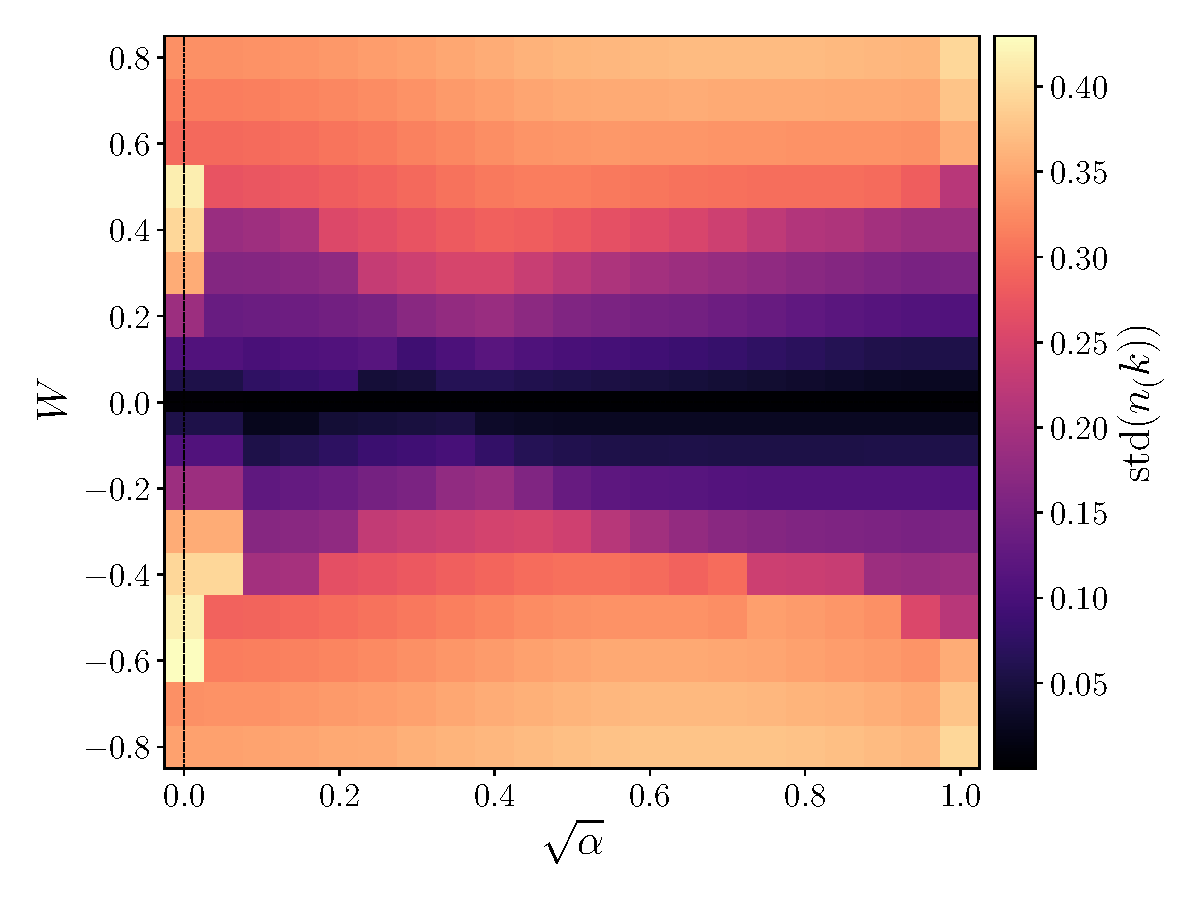
\includegraphics[width=0.5\textwidth]{plots/density_third_third_std_mesh.pdf}
    \caption{Standard deviation of $n(\mathbf{k})$ over the Brillouin zone as a function of $\alpha$ and $W$, at $\nu=\frac{2}{3}$.}\label{fig:third_third_density}
\end{figure}

Figure~\ref{fig:third_third_density} shows that the occupation is essentially flat at $W\approx 0$, while its standard deviation grows large at large $|W|$, confirming the expected Fermi-liquid character of the large-$|W|$ phases. The gapless VP phase likewise shows a non-flat occupation, consistent with Fermi-liquid behavior there. Two additional regions of low standard deviation stand out, surviving up to a discontinuity at relatively large $|W|$. The lower of these regions may correspond to an IVC phase undergoing a Stoner-like transition into a FL state analogous to the case of the depolarizing transition from the VP state, but with a different order parameter. This would agree with Ref.~\cite{raines2024unconventional}, where the VP state is expected to prevail at $\alpha < 0$ and the IVC at $\alpha > 0$, both with phase transitions of the same nature. A schematic summary including these candidate phases is given in Fig.~\ref{fig:summary}.
The larger--$\alpha$ flat occupation region is not studied in detail here.

\subsection{Screening of the interaction}

\begin{figure}[htbp]
    \centering
    \begin{subfigure}{0.45\textwidth}
        \centering
        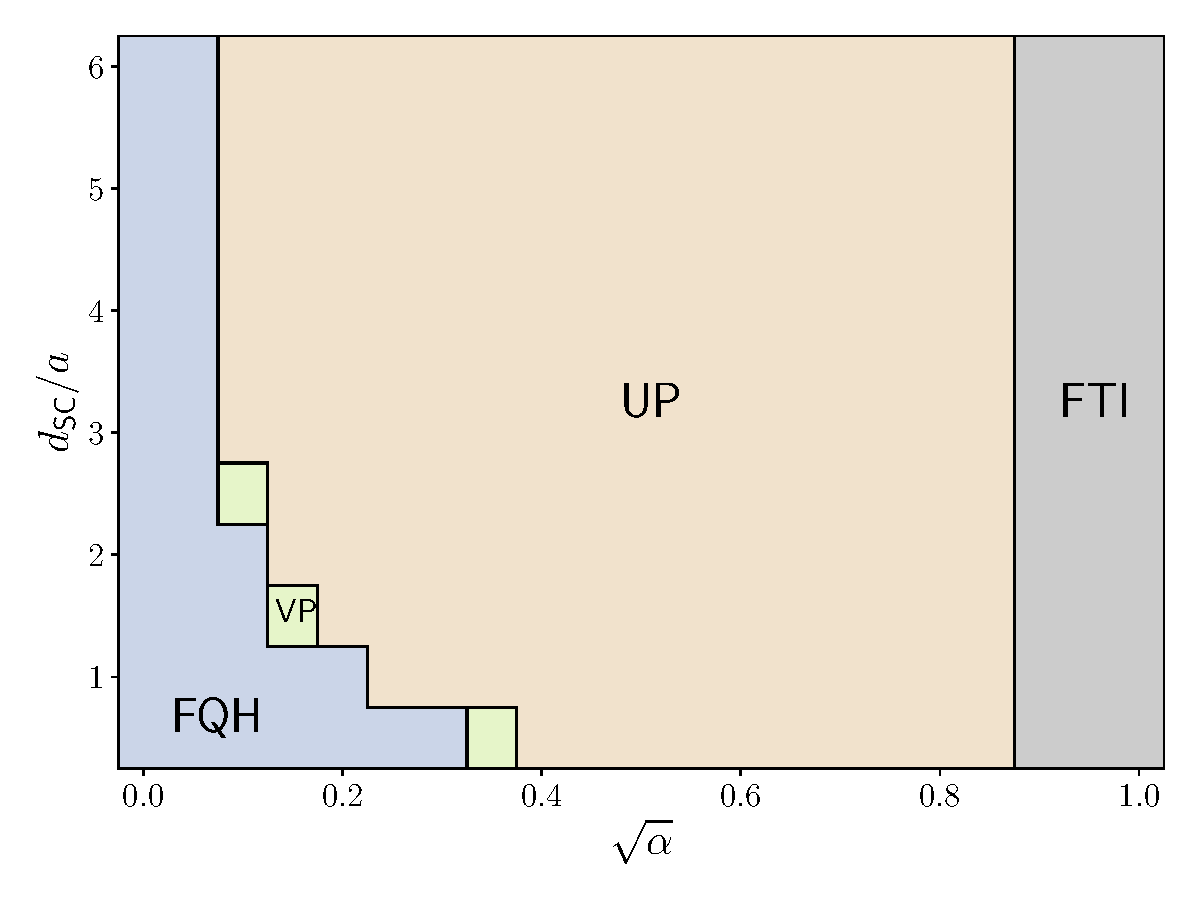
\includegraphics[width=1.0\textwidth]{plots/third_third_screening_alpha_vs_d_phase_diagram.pdf}
        \subcaption{$\alpha$ vs.\ $d_{\text{SC}}/a$, at $l_{\text{RK}} = 0$}\label{fig:third_third_screening_alpha_vs_d_phase_diagram_a}
    \end{subfigure}
    \begin{subfigure}{0.45\textwidth}
        \centering
        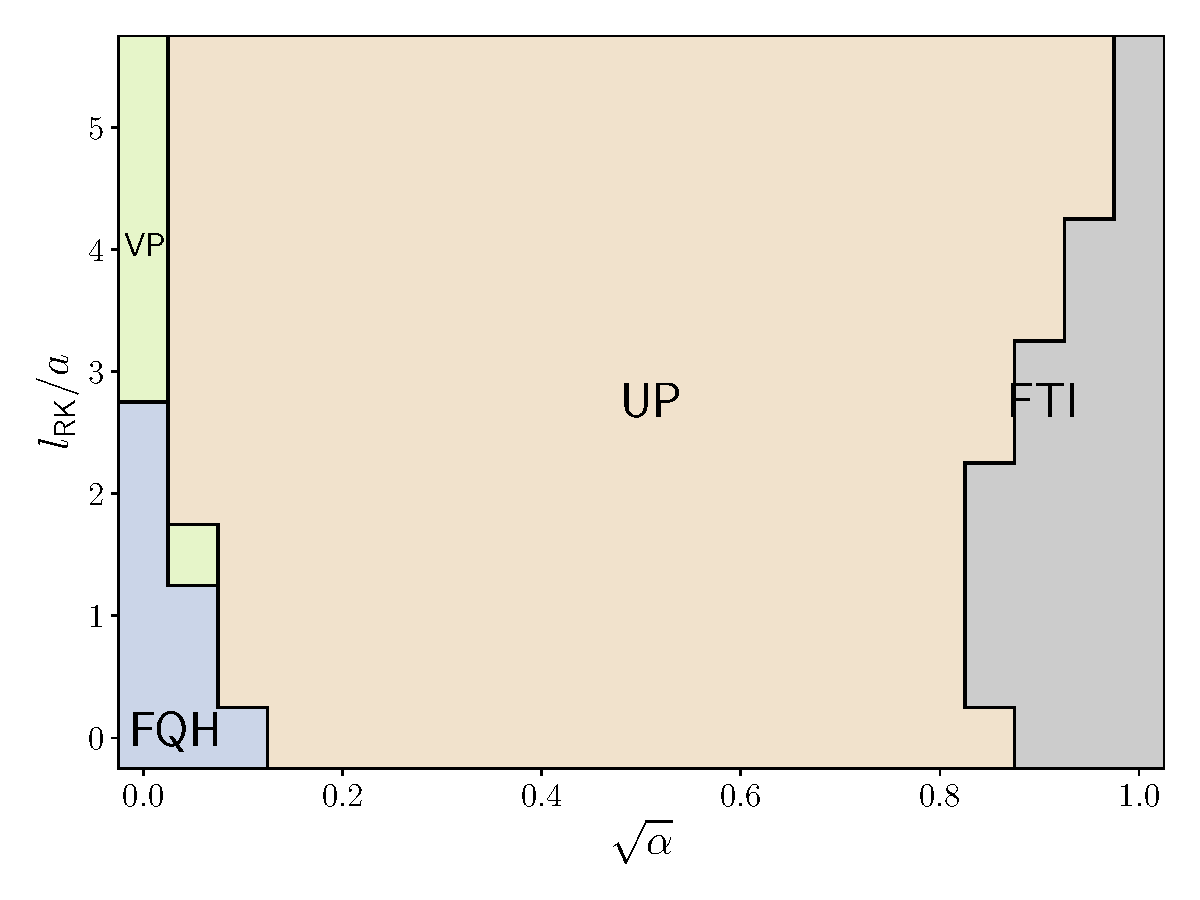
\includegraphics[width=1.0\textwidth]{plots/third_third_screening_alpha_vs_lRK_phase_diagram_d5.01.pdf}
        \subcaption{$\alpha$ vs.\ $l_{\text{RK}}/a$, at $d_{\text{SC}} = 2a$}\label{fig:third_third_screening_alpha_vs_lRK_phase_diagram_b}
    \end{subfigure}
    \caption{Phase diagrams of the $\nu = \frac{2}{3}$ filling at $W=0$ with respect to the screening parameters.}\label{fig:third_third_screening_alpha_vs_d_phase_diagram}
\end{figure}

The stability of the topological phases was tested against the two screening parameters $d_{\text{SC}}$ and $l_{\text{RK}}$. Figure~\ref{fig:third_third_screening_alpha_vs_d_phase_diagram_a} shows the extent of the phases at $W=0$ as a function of $\alpha$ and the screening length $d_{\text{SC}}$. Two conclusions follow. First, the $\alpha$-stability of the FQH phase decreases monotonically with increasing $d_{\text{SC}}$, in agreement with the analytic mean-field estimate, where increasing $d_{\text{SC}}$ shifts the $\alpha_c$ phase boundary in the same direction. Second, no corresponding change in the stability of the FTI phase is visible.

Figure~\ref{fig:third_third_screening_alpha_vs_lRK_phase_diagram_b} shows the analogous dependence on $l_{\text{RK}}$ at $W=0$. Here the stability of both topological phases varies: the FQH phase again becomes less stable with increasing $l_{\text{RK}}$, while the FTI phase instead shows a non-monotonic dependence, with a maximum of stability at finite $l_{\text{RK}}$.

\begin{figure}[htbp]
\centering
\begin{tikzpicture}[
    node distance = 0.6cm and 1.25cm, % Vertical and Horizontal spacing
    arrowstyle/.style={->, >=Stealth, thick, color=ethpetrol},
    labelstyle/.style={font=\small\sffamily, fill=white, inner sep=2pt, rounded corners=1pt, draw=ethpetrol, align=center}
]
    % --- ROW 1 ---
    % Subfigure 1
    \node (sub1) {
        \begin{subfigure}{0.4\textwidth}
            \centering
            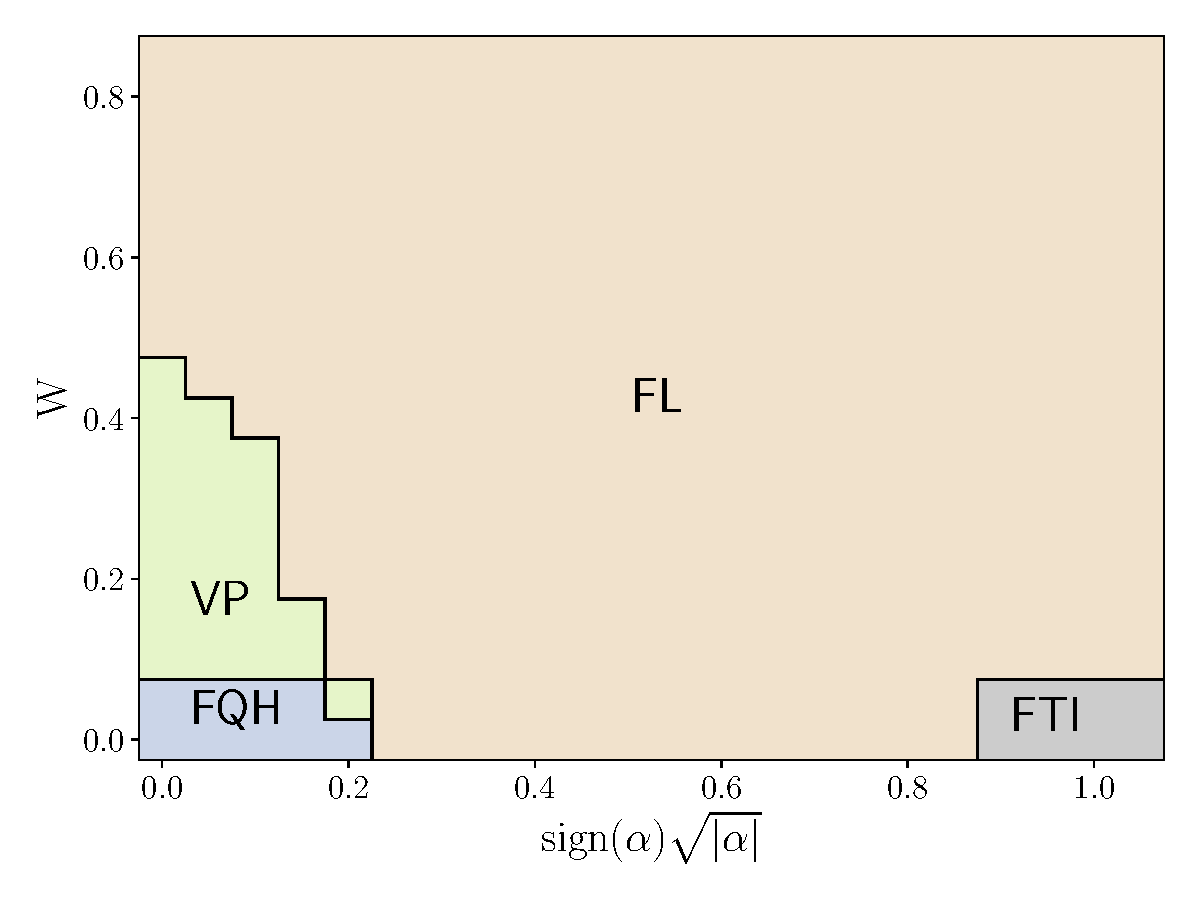
\includegraphics[width=\textwidth]{plots/third_third_screening_alpha_vs_W_phase_diagram_d2.51_lRK0.00.pdf}
            \caption{}
            \label{fig:third_third_screening_alpha_vs_W_phase_diagram_a}
        \end{subfigure}
    };

    % Subfigure 2 (Placed to the right of Subfigure 1)
    \node[right=of sub1] (sub2) {
        \begin{subfigure}{0.4\textwidth}
            \centering
            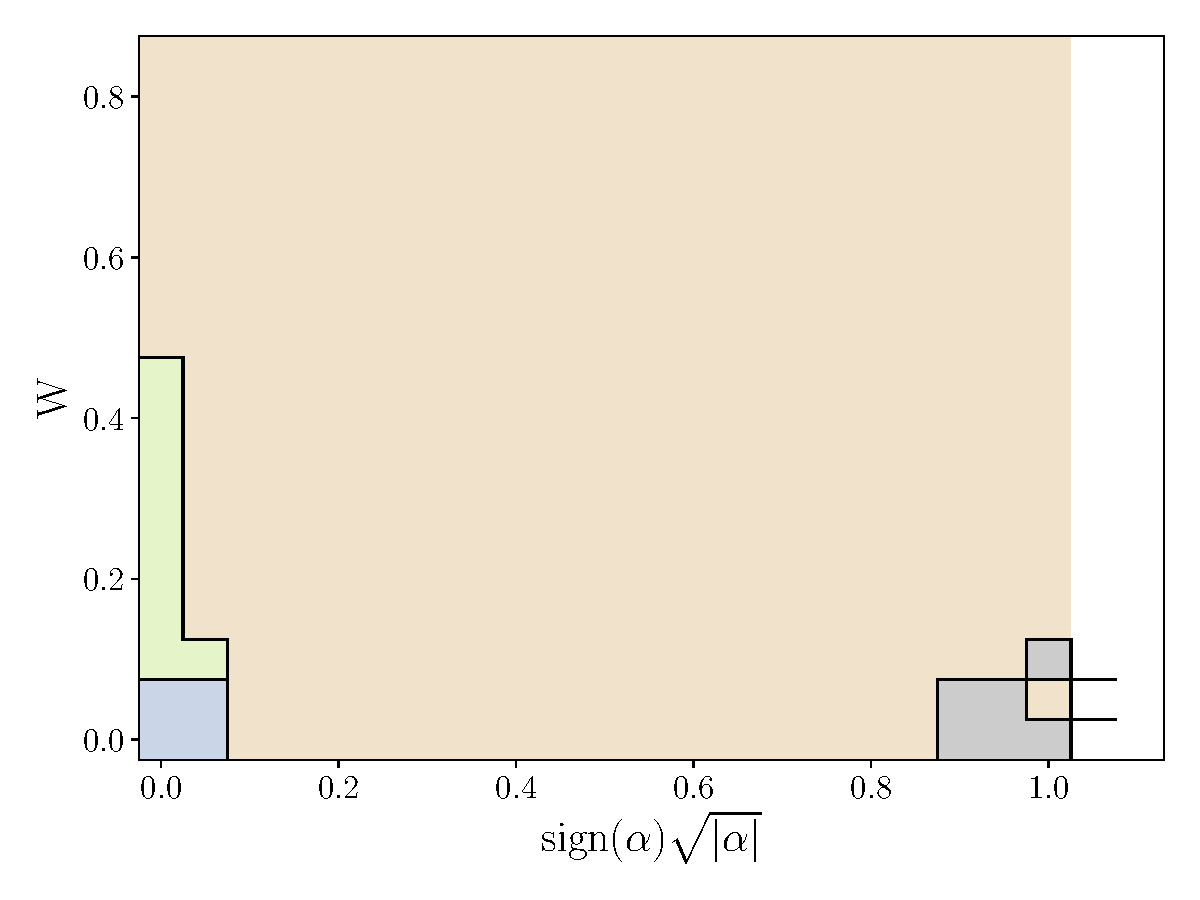
\includegraphics[width=\textwidth]{plots/third_third_screening_alpha_vs_W_phase_diagram_d15.04_lRK0.00.pdf}
            \caption{}
            \label{fig:third_third_screening_alpha_vs_W_phase_diagram_b}
        \end{subfigure}
    };

    % --- ROW 2 ---
    % Subfigure 3 (Centered below the space between sub1 and sub2)
    \node[below=of $(sub1.south)!0.5!(sub2.south)$] (sub3) {
        \begin{subfigure}{0.4\textwidth}
            \centering
            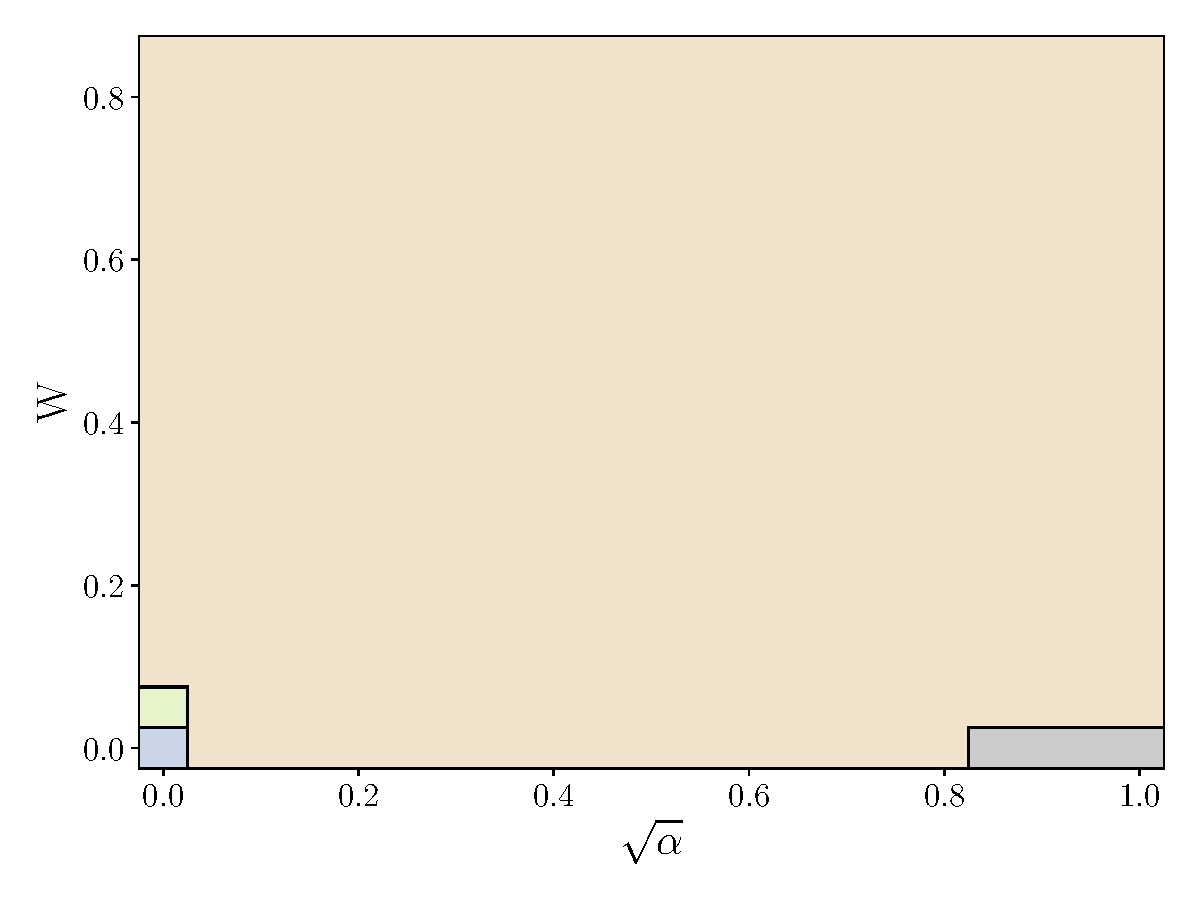
\includegraphics[width=\textwidth]{plots/third_third_screening_alpha_vs_W_phase_diagram_d15.04_lRK5.01.pdf}
            \caption{}
            \label{fig:third_third_screening_alpha_vs_W_phase_diagram_c}
        \end{subfigure}
    };

    % --- ARROWS ---
    % Arrow 1: Plot 1 -> Plot 2
    \draw[arrowstyle] ($(sub1.east) + (-5pt,0)$) -- ($(sub2.west) + (15pt,0)$) 
        node[midway, labelstyle] {$\mathbf{d_{\mathrm{SC}} \nearrow }$};

    % Arrow 2: Plot 2 -> Plot 3 (Connects bottom of Plot 2 to right edge of centered Plot 3)
    \draw[arrowstyle] ($(sub2.south west) + (15pt,30pt)$) -- ($(sub3.north) + (0, -5pt)$)%($(sub2.south west) + (10pt,-5pt)$) -- ($(sub3.north) + (0, 5pt)$) 
        node[midway, labelstyle] {$\mathbf{l_{\mathrm{RK}} \nearrow }$};

\end{tikzpicture}
\caption{Phase diagrams of the $\nu = \frac{2}{3}$ filling in the $\alpha$--$W$ plane with different screening $d_{\text{SC}}$ and $l_{\text{RK}}$. Arrows indicate the direction of change of the parameters.\ (a) $d_{\text{SC}} = 1a$, $l_{\text{RK}} = 0$.\ (b) $d_{\text{SC}} = 6a$, $l_{\text{RK}} = 0$.\ (c) $d_{\text{SC}} = 6a$, $l_{\text{RK}} = 2a$.}\label{fig:third_third_screening_alpha_vs_W_phase_diagram_mindmap}
\end{figure}

Figure~\ref{fig:third_third_screening_alpha_vs_W_phase_diagram_mindmap} shows the full $\alpha$--$W$ phase diagram at different screening parameters, allowing the $W$-stability to be examined alongside the $\alpha$-stability. The main conclusion is that the $W$-stability is essentially independent of $d_{\text{SC}}$, but decreases significantly with increasing $l_{\text{RK}}$. This is particularly relevant for the FTI phase, where seemingly to gain $\alpha$-stability by tuning the screening, one must sacrifice the $W$-stability.

\section{\texorpdfstring{Phase diagram for $\nu = 1$}{Phase diagram for nu = 1/2 + 1/2}}

While fractional topological states are not expected at $\nu=1$ in the LLL, this filling has been studied in the literature and serves as a useful benchmark for the method, as well as a reference point for $n=1$ LL calculations in Chapter~\ref{ch:results_1LL}~\cite{das2025fractional, kwan2025textured}.

\begin{figure}[htbp]
    \centering
    \begin{subfigure}{0.45\textwidth}
        \centering
        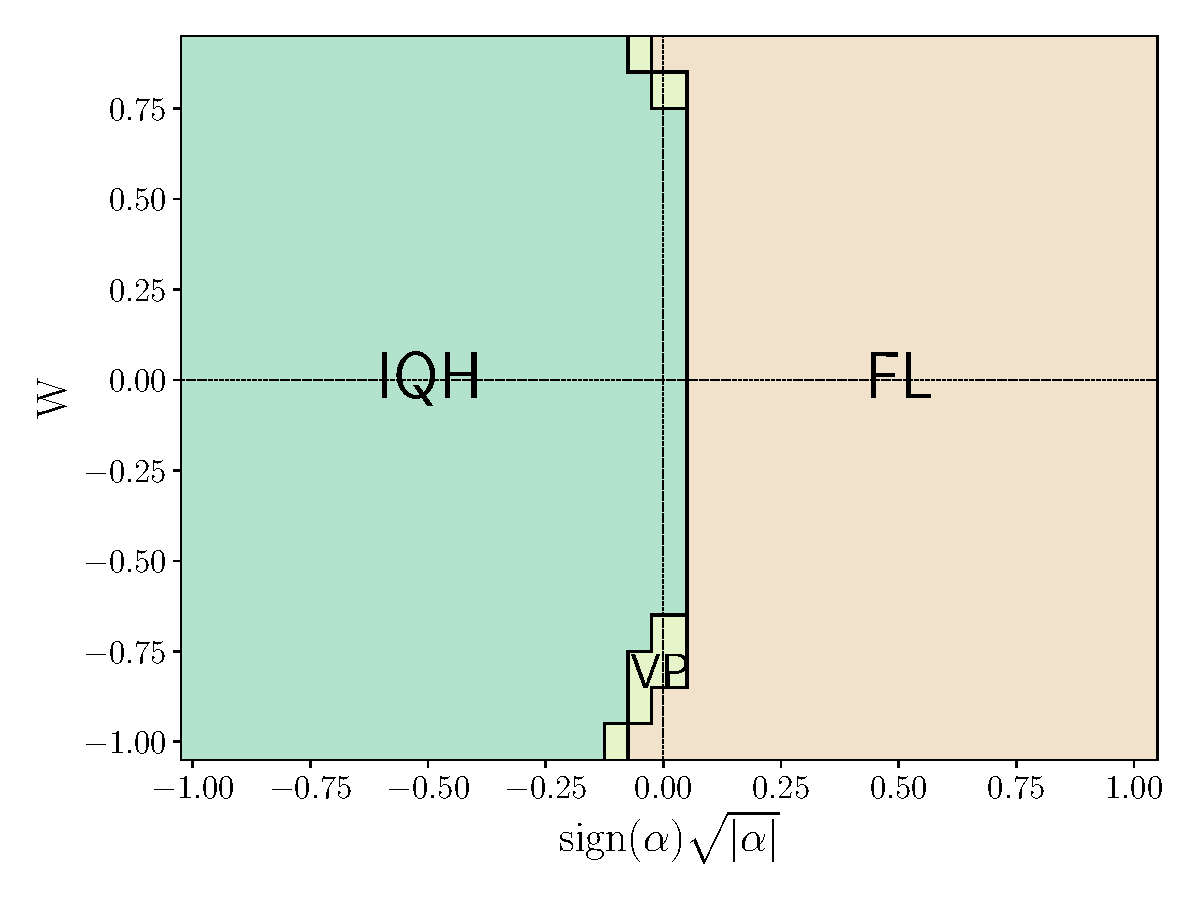
\includegraphics[width=1.0\textwidth]{plots/half_half_phase_diagram.pdf}
        \subcaption{$U(q=0)\neq 0$}\label{fig:half_half_phase_diagram}
    \end{subfigure}
    \begin{subfigure}{0.45\textwidth}
        \centering
        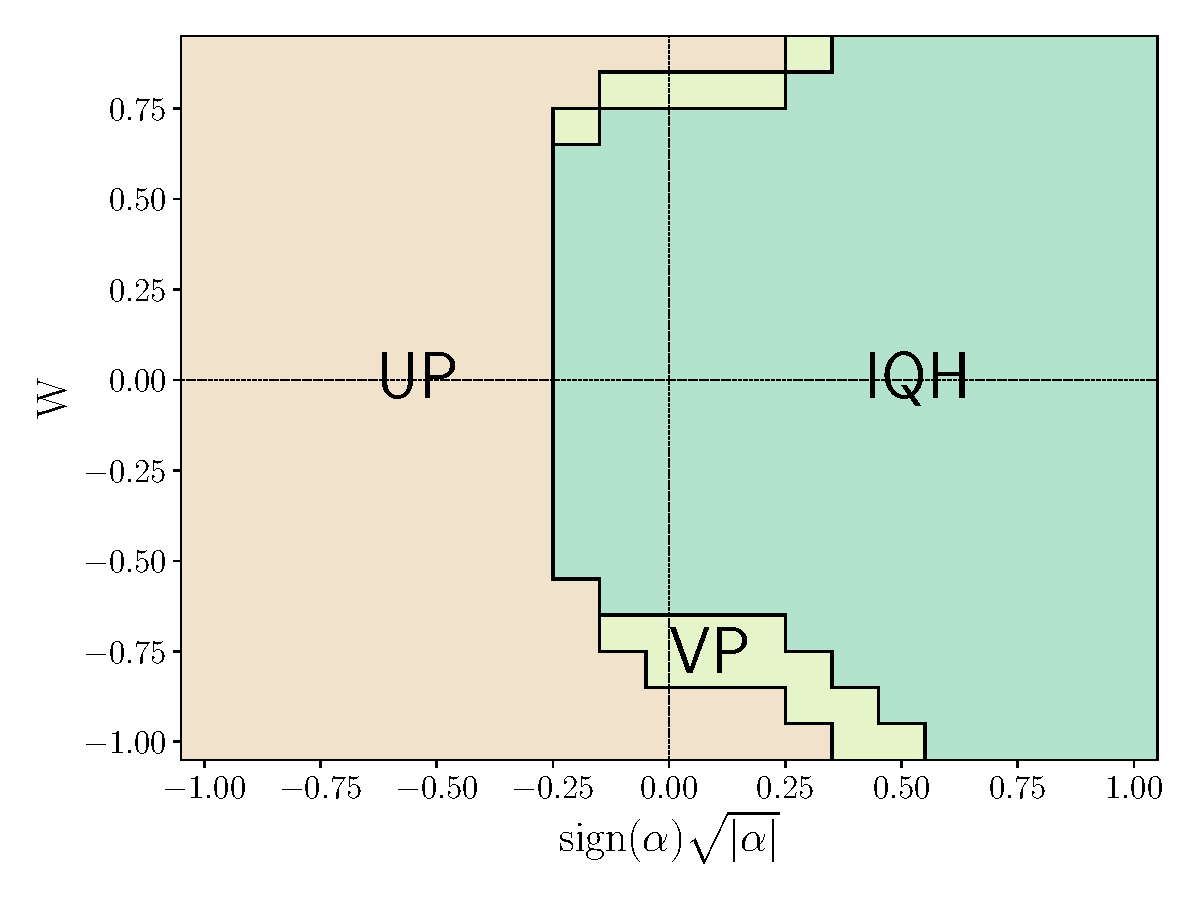
\includegraphics[width=1.0\textwidth]{plots/half_half_q0_phase_diagram.pdf}
        \subcaption{$U(q=0) = 0$}\label{fig:half_half_q0_phase_diagram}
    \end{subfigure}
    \begin{subfigure}{0.45\textwidth}
        \centering
        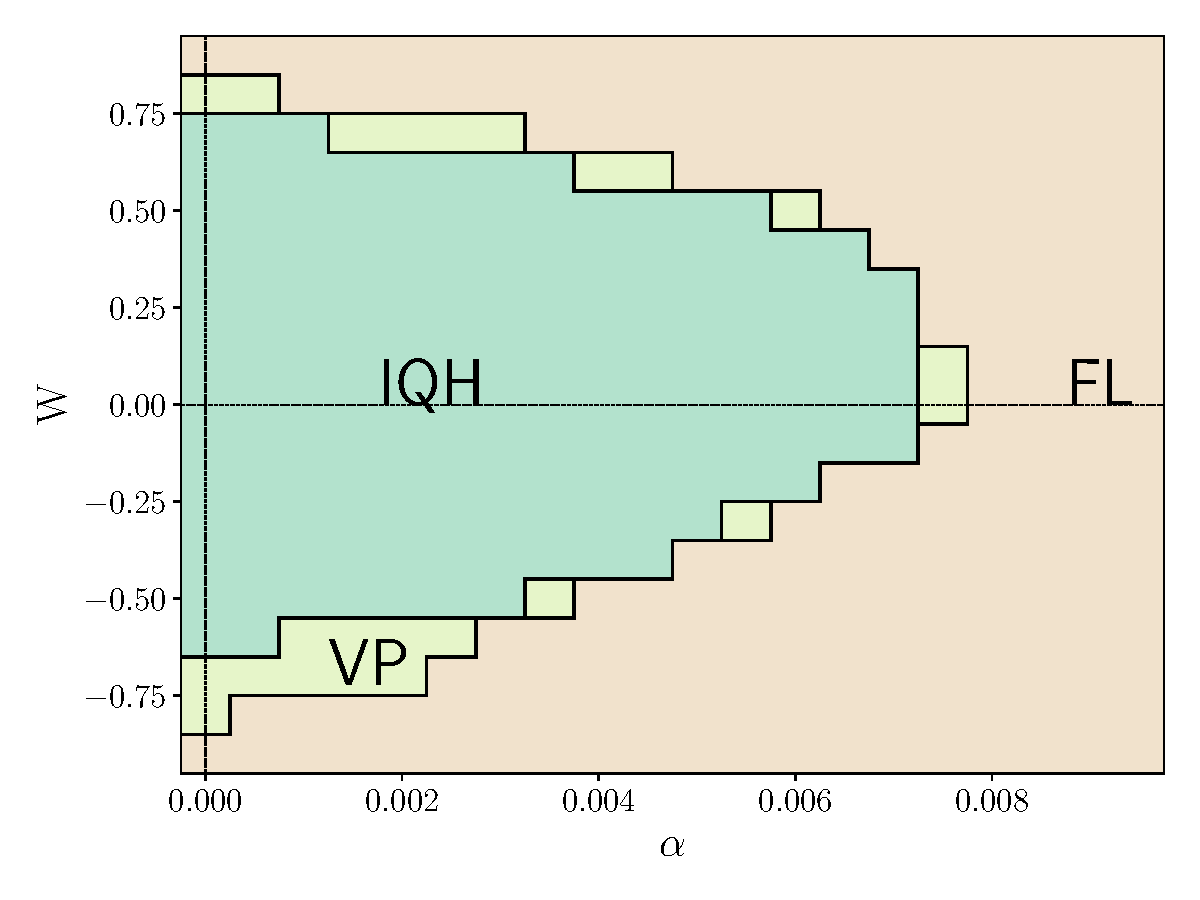
\includegraphics[width=1.0\textwidth]{plots/half_half_zoom_phase_diagram.pdf}
        \subcaption{Zoom-in on the IQH ($U(q=0) \neq 0$)}\label{fig:half_half_zoom_phase_diagram}
    \end{subfigure}
    \begin{subfigure}{0.45\textwidth}
        \centering
        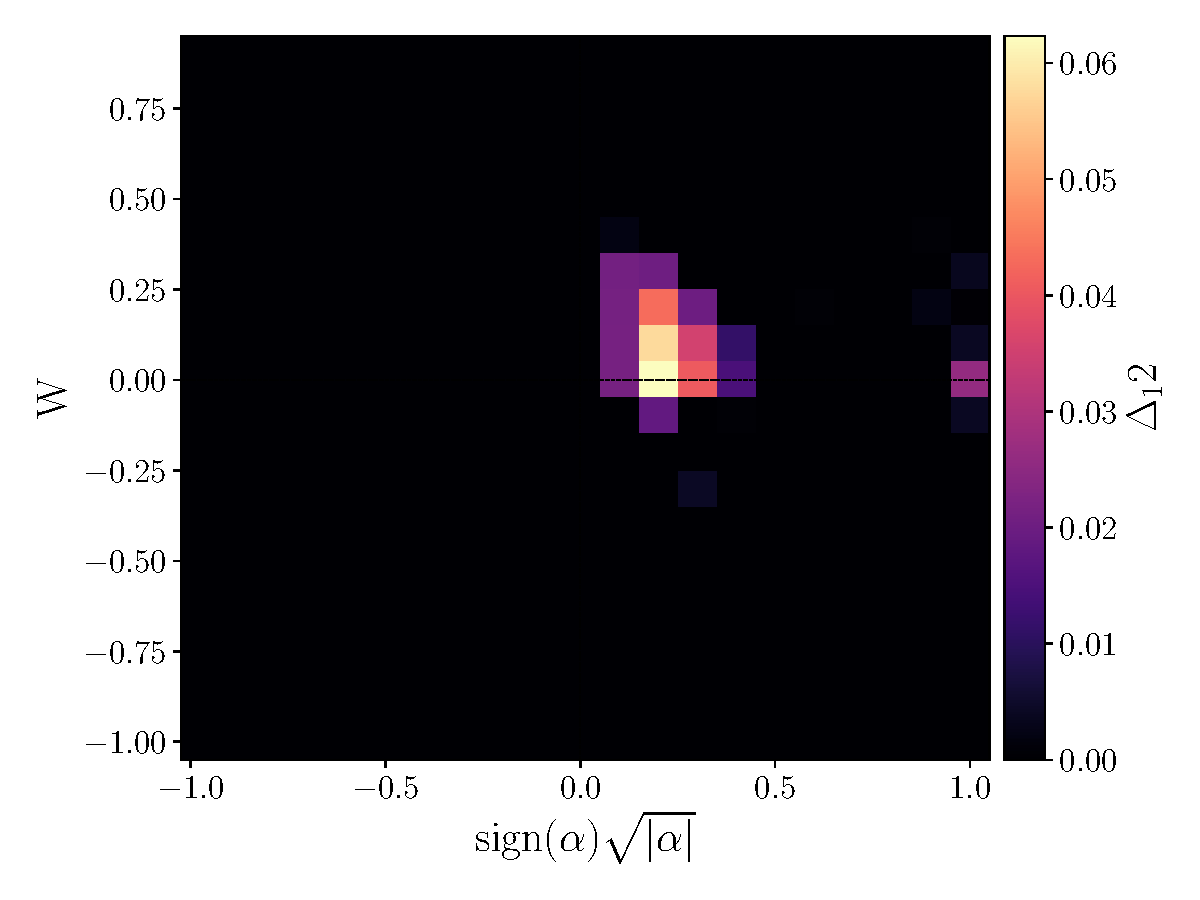
\includegraphics[width=1.0\textwidth]{plots/half_half_gap_n12.pdf}
        \subcaption{$\Delta_{12}$ gap, $U(q=0)\neq 0$}\label{fig:half_half_gap_n12}
    \end{subfigure}
    \caption{Phase diagrams of the $\nu = 1$ filling. UP:\@ general unpolarized state. IQH:\@ valley-polarized integer quantum Hall state. See Fig.~\ref{fig:summary} for a schematic identification of the UP regions.}\label{fig:half_half_phases}
\end{figure}

Figure~\ref{fig:half_half_phases} shows the resulting phase diagram. With $U(\mathbf{q}=0) \neq 0$, similarly to the $\nu=\frac{2}{3}$, a valley-polarized region is found at low $\alpha$, giving way to a gapless non-polarized phase at larger $\alpha$ or larger $|W|$. Due to integer filling, the valley-polarized phase is the IQH state at $\nu = 1 + 0$ and with $\Delta_1 > 0$. The resulting phase boundary is consistent with past results~\cite{kwan2025textured} and with the numerical mean-field estimate, within the same order of magnitude.

The nature of the high--$\alpha$ gapless state can again be discussed in light of the literature and the momentum-occupation function. In the $\alpha = 1$, $W=0$ limit, the $\nu = \tfrac{1}{2} + \tfrac{1}{2}$ state is known to consist of decoupled composite Fermi liquids, $\ket{\text{CFL}} \otimes \overline{\ket{\text{CFL}}}$, while at large bandwidth $|W|$, where kinetic energy dominates, it becomes a pair of Fermi liquids, $\ket{\text{FL}} \otimes \overline{\ket{\text{FL}}}$. The phase transition and boundary between these two states, and the nature of the intermediate states once $\alpha \neq 1$ cannot be resolved with the limited extent of the simulations performed here.

With $U(\mathbf{q}=0) = 0$, the phase diagram shown in Figure~\ref{fig:half_half_q0_phase_diagram} is again inverted. While containing the same phases (IQH, VP and UP) and the same $W$ dependence, now the ground state is unpolarized at low $\alpha$ while the IQH is prevalent at high $\alpha$.

\subsection{\texorpdfstring{Intermediate--$\alpha$ and high-$|W|$ phases}{Intermediate-alpha and high-W phases}}\label{sec:intermediate_alpha_half_half}


\subsubsection{Finite size effects}
Returning to the $U(\mathbf{q}=0)\neq 0$ case, at intermediate $\alpha$, a $\Delta_{12} \neq 0$ gap is found (Fig.~\ref{fig:half_half_gap_n12}), similarly to the $\nu=\tfrac{2}{3}$ system. Such degeneracy does not correspond to any topologically nontrivial state and phase winding is not present. Since the degeneracy is equal to the number of unit cells, it suggests complete translational symmetry breaking in a form of phase separation. It is important to note that the gap is nonzero only for $W \geq 0$, which suggests that the state might stem from finite size effects. An IVC state was reported in this region of the phase diagram by Ref.~\cite{kwan2025textured}, with the peak of the IVC order parameter $\Delta_q$ at $q = \mathbf{Q_0} = (\tfrac{Q}{2},\tfrac{Q}{2})$. The default $3\times 4$ BZ sampling studied here does not contain this point, which might result in favoring other competing phases. To clarify the nature of the state an additional calculation is performed at the same filling, with $N_\phi=10$, in a tilted lattice of Figure~\ref{fig:bz_sampling_10}. This lattice, on the other hand, contains the $\mathbf{Q_0}$ point. The sampling is invariant under the $\mathbf{Q_0}$ shift, and is also more isotropic with $\tfrac{|T_1|}{|T_2|}$ closer to $1$.

\begin{figure}[htbp]
    \centering
    \begin{subfigure}{0.45\textwidth}
        \centering
        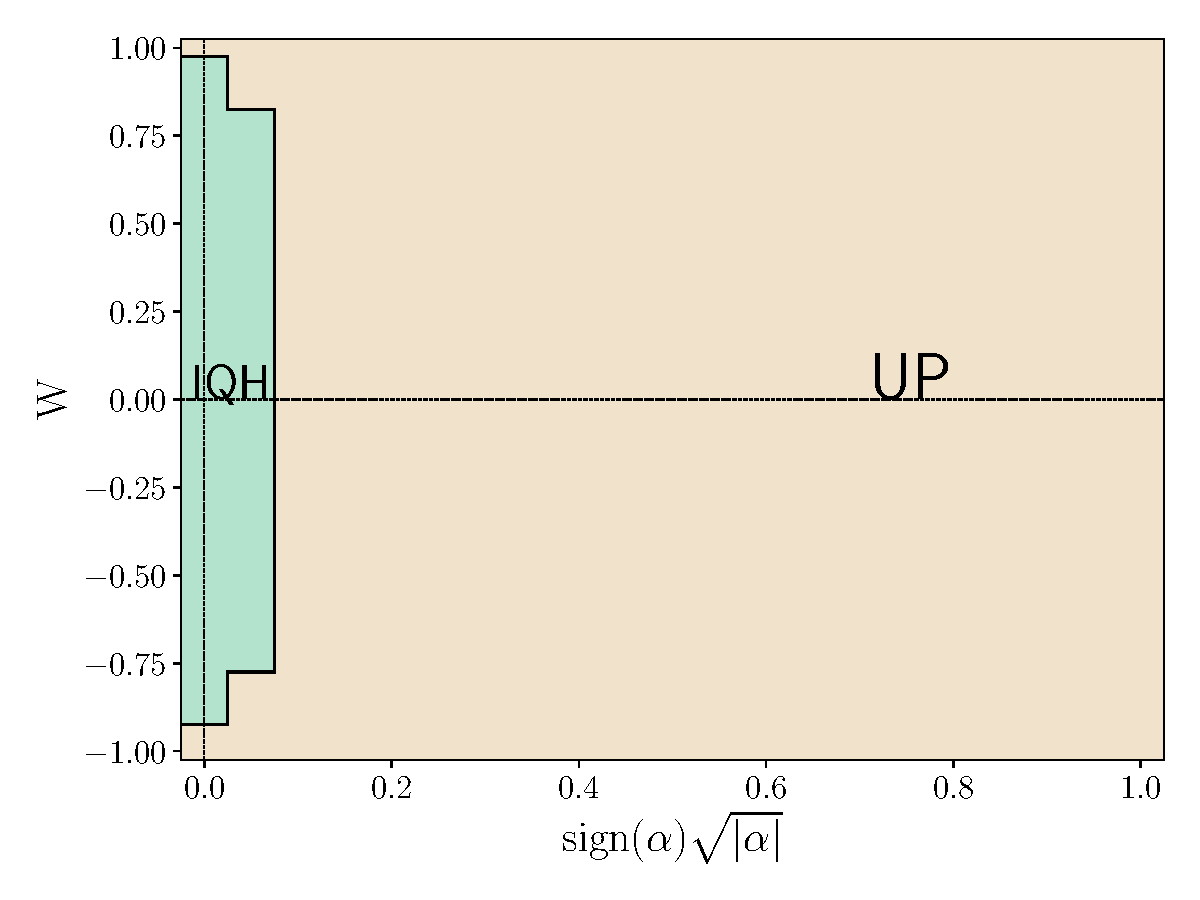
\includegraphics[width=1.0\textwidth]{plots/half_half_tilted_phase_diagram.pdf}
        \subcaption{Phase diagram}\label{fig:half_half_tilted_phase_diagram}
    \end{subfigure}
    \begin{subfigure}{0.45\textwidth}
        \centering
        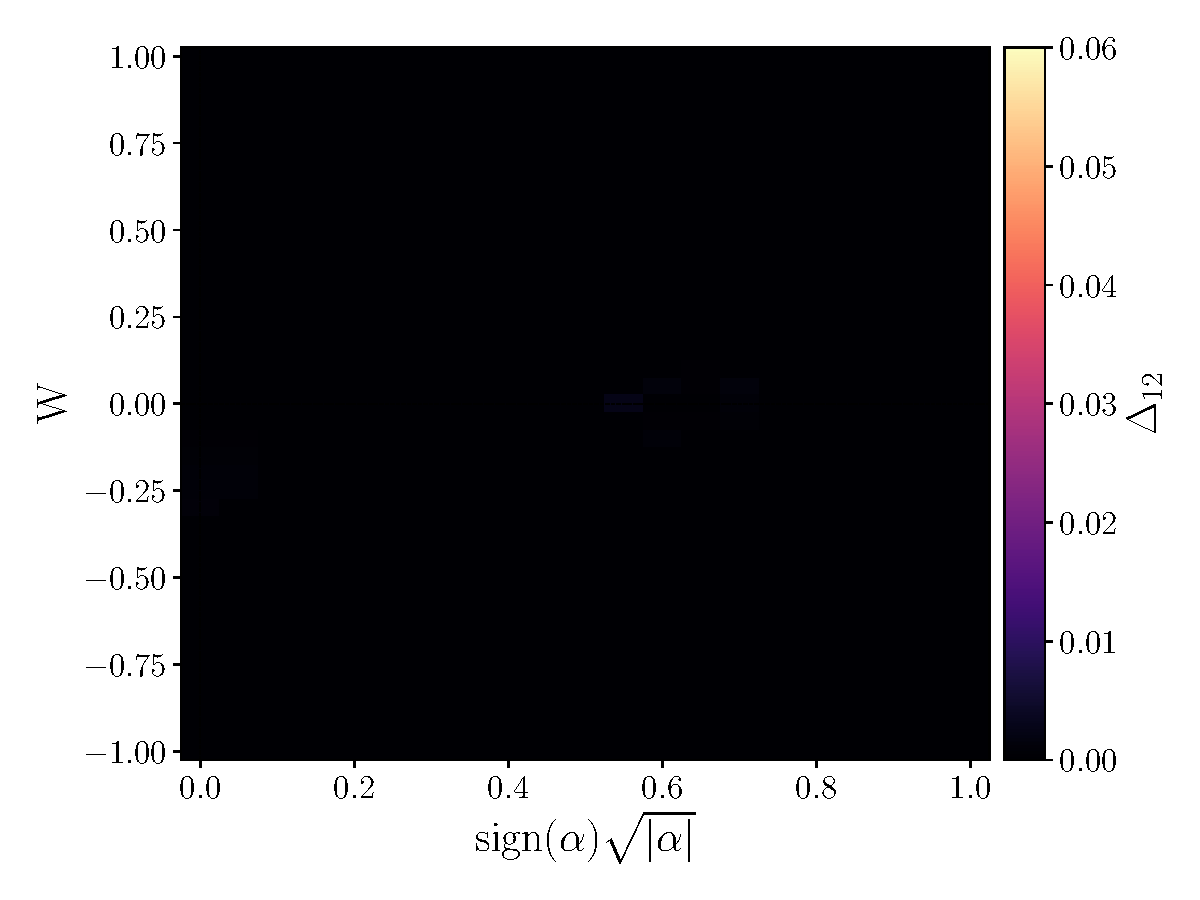
\includegraphics[width=1.0\textwidth]{plots/half_half_tilted_gap_n12.pdf}
        \subcaption{$\Delta_{12}$}\label{fig:half_half_tilted_gap_12}
    \end{subfigure}
    \begin{subfigure}{0.45\textwidth}
        \centering
        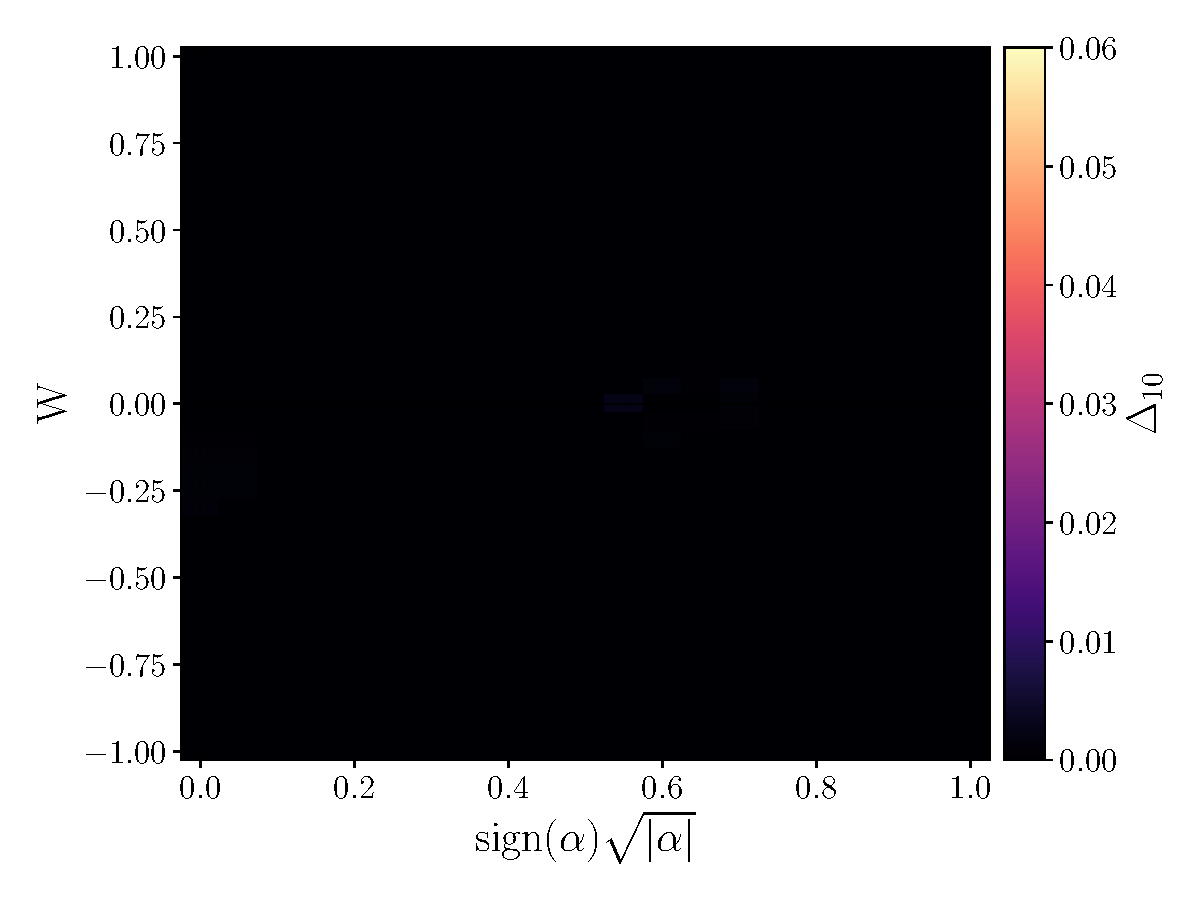
\includegraphics[width=1.0\textwidth]{plots/half_half_tilted_gap_n10.pdf}
        \subcaption{$\Delta_{10}$}\label{fig:half_half_tilted_gap_10}
    \end{subfigure}
    \caption{Phase diagram and gaps in a $\nu=1$ system with tilted boundary conditions of Fig.~\ref{fig:bz_sampling_10}.}\label{fig:half_half_tilted}
\end{figure}

The results are shown in Figure~\ref{fig:half_half_tilted}. First, in this system both the $\Delta_{12}$ gap --- as a comparison with the $3\times 4$ system --- and the $\Delta_{10}$ gap --- corresponding now to the number of unit cells in the system --- are strictly $0$, confirming that the gapped phase is favored only due to finite size effects or anisotropy of the cluster. Second, in Figure~\ref{fig:half_half_tilted_phase_diagram} the phase diagram is perfectly symmetric with respect to $W=0$, confirming the prediction of \S\ref{sec:symmetries} to be exact when the BZ sampling is invariant under the $\mathbf{Q_0}$ shift.


\subsubsection{Momentum-occupation function}
\begin{figure}[htbp]
    \centering
    \begin{subfigure}{0.45\textwidth}
        \centering
        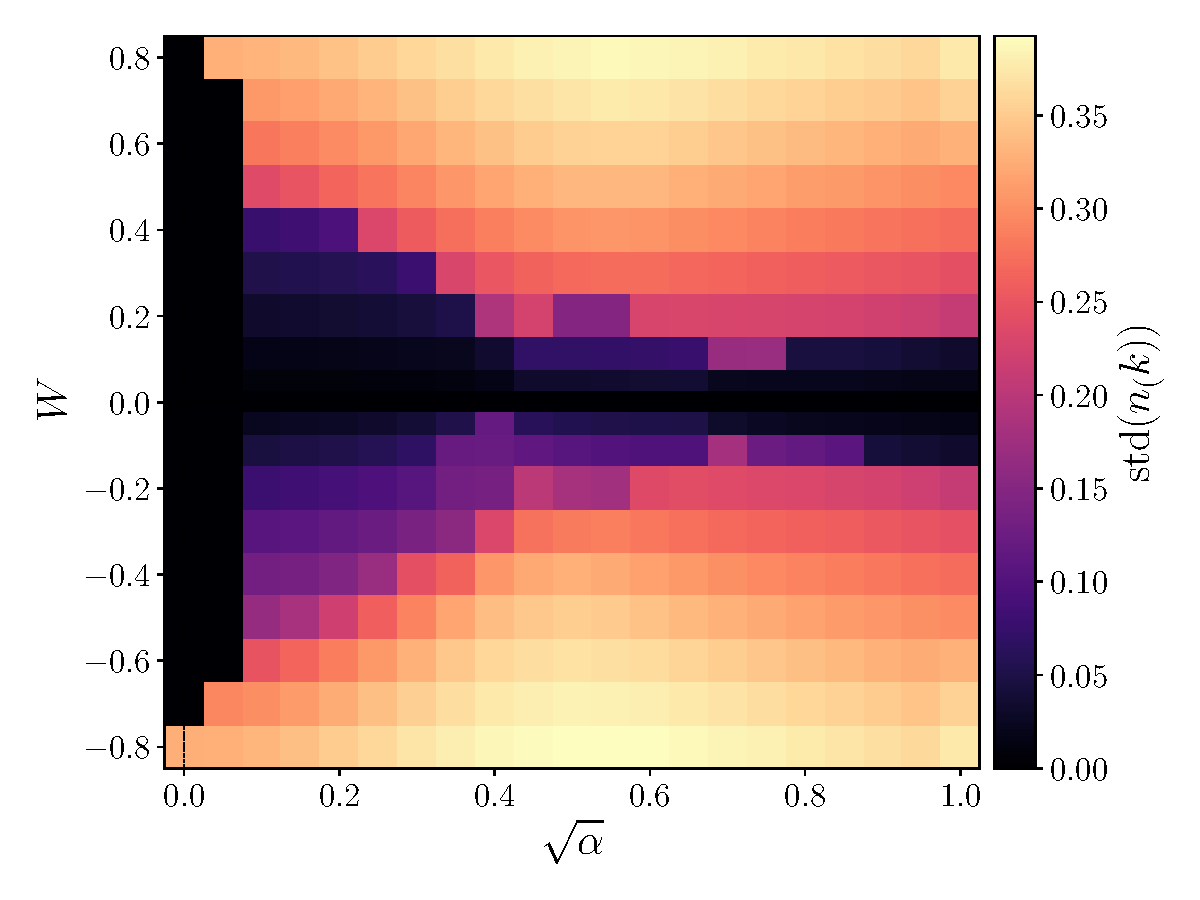
\includegraphics[width=1.0\textwidth]{plots/density_half_half_std_mesh.pdf}
        \subcaption{Standard deviation of $n(\mathbf{k})$ vs.\ $\alpha$, $W$}\label{fig:half_half_density_std}
    \end{subfigure}
    \begin{subfigure}{0.45\textwidth}
        \centering
        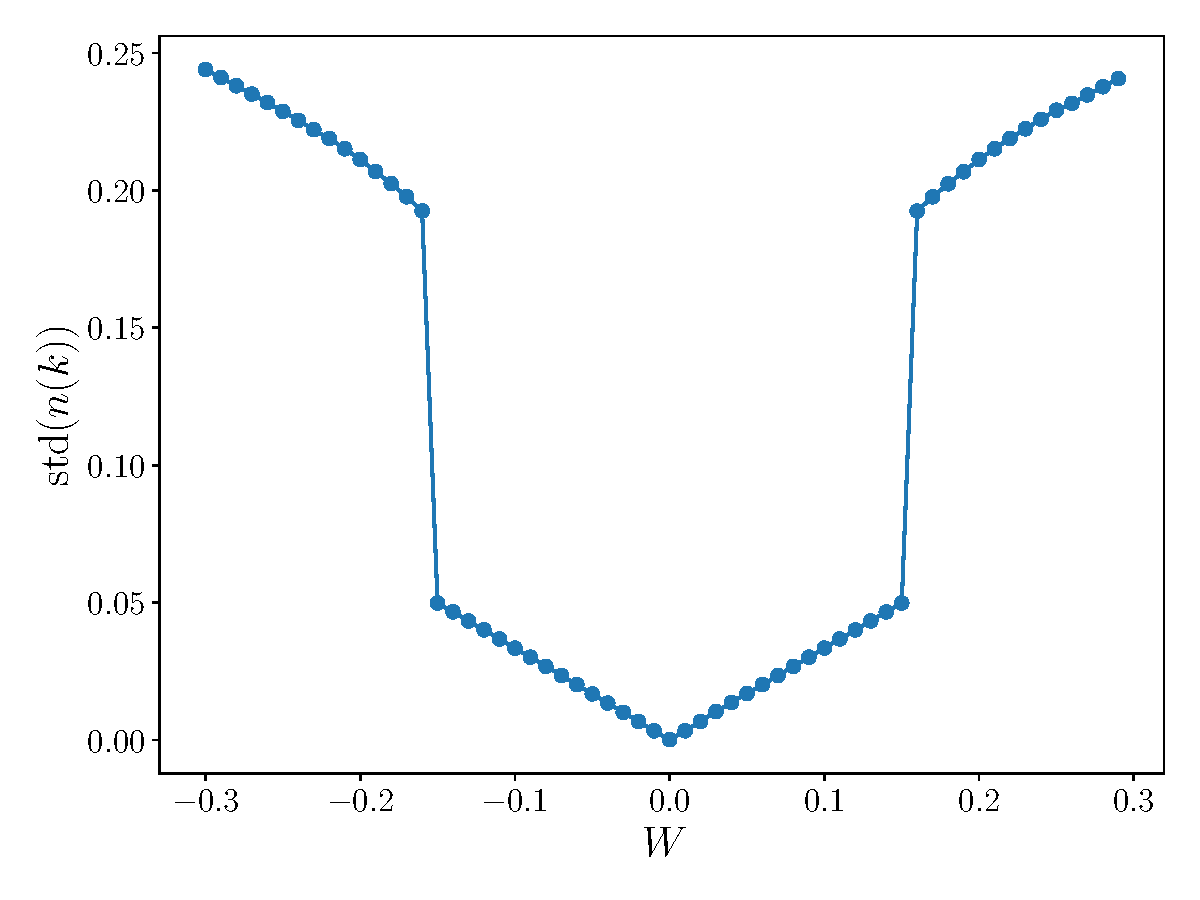
\includegraphics[width=1.0\textwidth]{plots/density_half_half_alpha1_std_cut_alpha_1.00.pdf}
        \subcaption{Cut of (a) at $\alpha=1$}\label{fig:half_half_density_cut}
    \end{subfigure}
    \begin{subfigure}{0.45\textwidth}
        \centering
        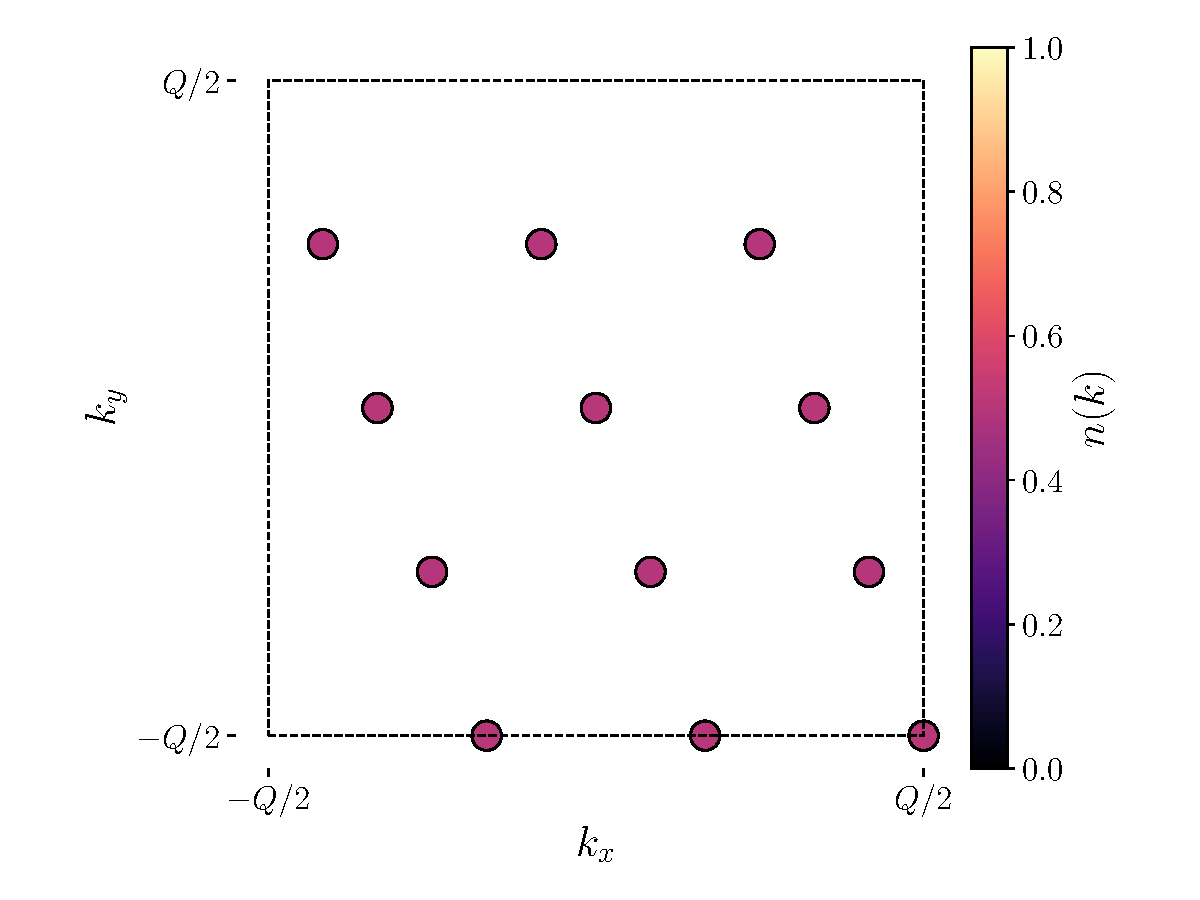
\includegraphics[width=1.0\textwidth]{plots/density_half_half_nk_W_0.00_alpha_1.00.pdf}
        \subcaption{$n(\mathbf{k})$ at $W=0.0$, $\alpha=1.0$\\ $\ket{\text{CFL}} \otimes \overline{\ket{\text{CFL}}}$}\label{fig:half_half_density_CFL}
    \end{subfigure}
    \begin{subfigure}{0.45\textwidth}
        \centering
        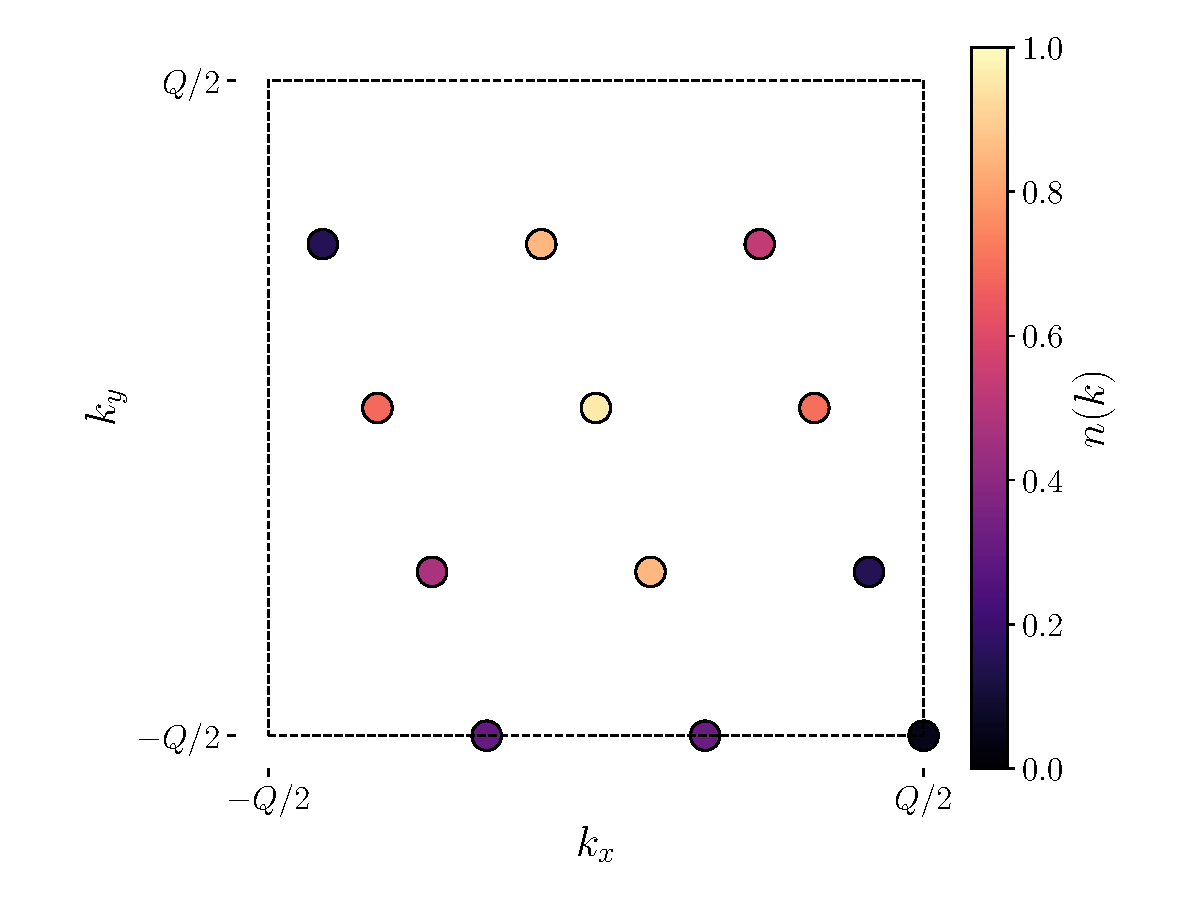
\includegraphics[width=1.0\textwidth]{plots/density_half_half_nk_W_0.50_alpha_1.00.pdf}
        \subcaption{$n(\mathbf{k})$ at $W=0.5$, $\alpha=1.0$\\ $\ket{\text{FL}} \otimes \overline{\ket{\text{FL}}}$}\label{fig:half_half_density_FL}
    \end{subfigure}
    \caption{The momentum-space occupation $n(\mathbf{k})$ for the $\nu=1$ filling, shown for an arbitrary valley.}\label{fig:half_half_density}
\end{figure}

Figure~\ref{fig:half_half_density} shows the standard deviation of $n(\mathbf{k})$ over the Brillouin zone. A large region of flat occupation is again observed at $\sqrt{\alpha} \in [0.05, 0.4]$, which, by comparison with the literature, may correspond to the IVC state, with a discontinuous transition to the Fermi liquid at higher $|W|$: while Kwan et al.~\cite{kwan2025textured} confirm the IVC phase, the transition itself is not reported there --- IVC being also found at higher $W$. The same discontinuity of $n(\mathbf{k})$ is found both at $W > 0$ and at $W < 0$ in both the default and the tilted cluster calculations, confirming that it is not caused by the phase-separated state found only in one of these four cases.

The IVC phase reported in Ref.~\cite{kwan2025textured} is a gapped Chern-texture insulator, while the state found here is consistently gapless. This is not incompatible with their result, since their Hartree--Fock gap is a charge gap, whereas the gap calculated here is a neutral gap, which is expected to be gapless in the IVC phase due to its Goldstone mode.


Additionally, a clear transition between $\ket{\text{CFL}} \otimes \overline{\ket{\text{CFL}}}$ and $\ket{\text{FL}} \otimes \overline{\ket{\text{FL}}}$ is seen at $\alpha=1$, with a jump in the standard deviation of $n(\mathbf{k})$ at $W \approx 0.17$ (Fig.~\ref{fig:half_half_density_cut}); an analogous transition for a single Landau level was studied by Barkeshli and McGreevy~\cite{barkeshli2012continuous}. The momentum-occupation function is shown explicitly on either side of this transition: it is flat at low $|W|$ (Fig.~\ref{fig:half_half_density_CFL}), and shows a clear Fermi surface at high $|W|$ (Fig.~\ref{fig:half_half_density_FL}).

\section{\texorpdfstring{Phase diagram for $\nu = \frac12$}{Phase diagram for nu = 1/2}}

For completeness, the $\nu = \tfrac{1}{2}$ filling was studied in an analogous way. No gapped topological order is expected here in the lowest Landau level, but the valley polarization is expected to behave qualitatively similarly to the other fillings considered above.

\begin{figure}[htbp]
    \centering
    \begin{subfigure}{0.45\textwidth}
        \centering
        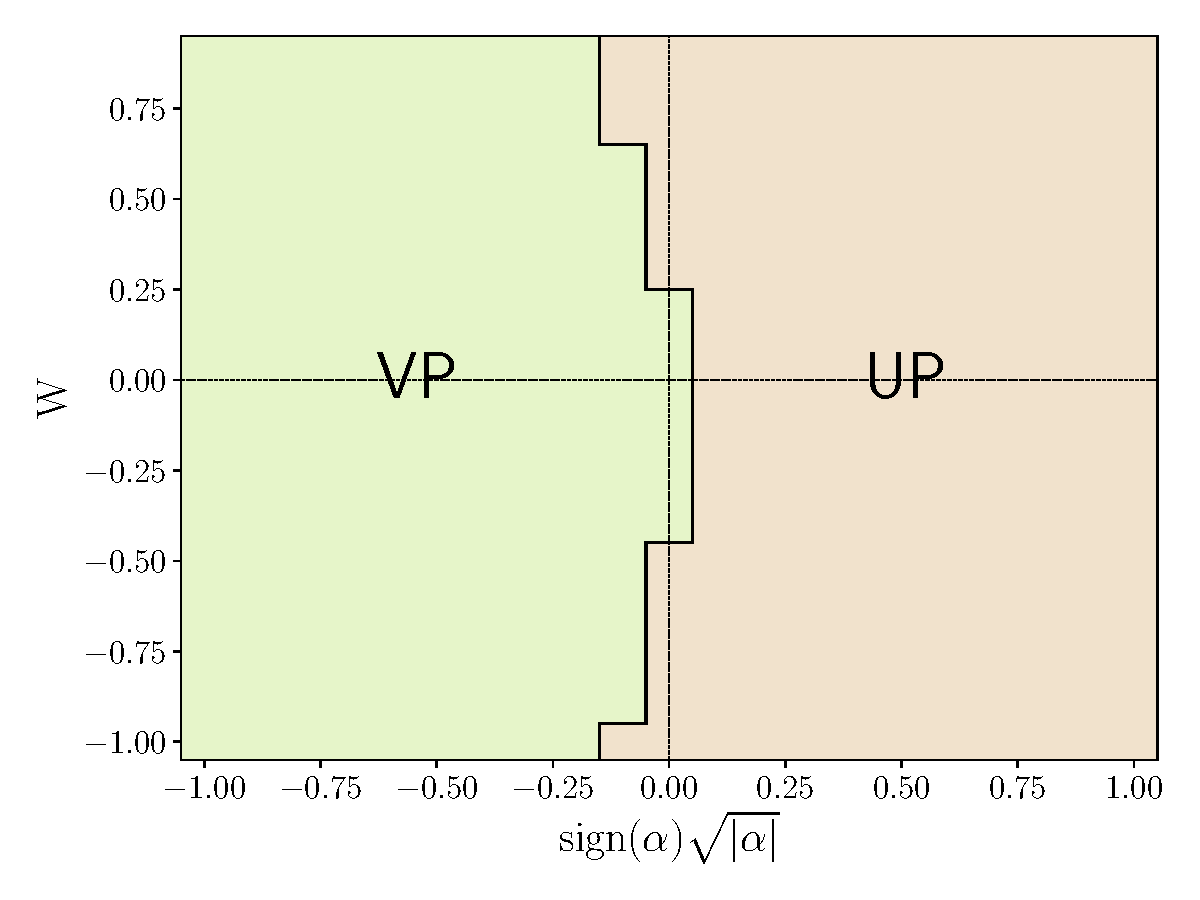
\includegraphics[width=1.0\textwidth]{plots/fourth_fourth_phase_diagram.pdf}
        \subcaption{$U(\mathbf{q}=0)\neq0$}\label{fig:fourth_fourth_phase_diagram}
    \end{subfigure}
    \begin{subfigure}{0.45\textwidth}
        \centering
        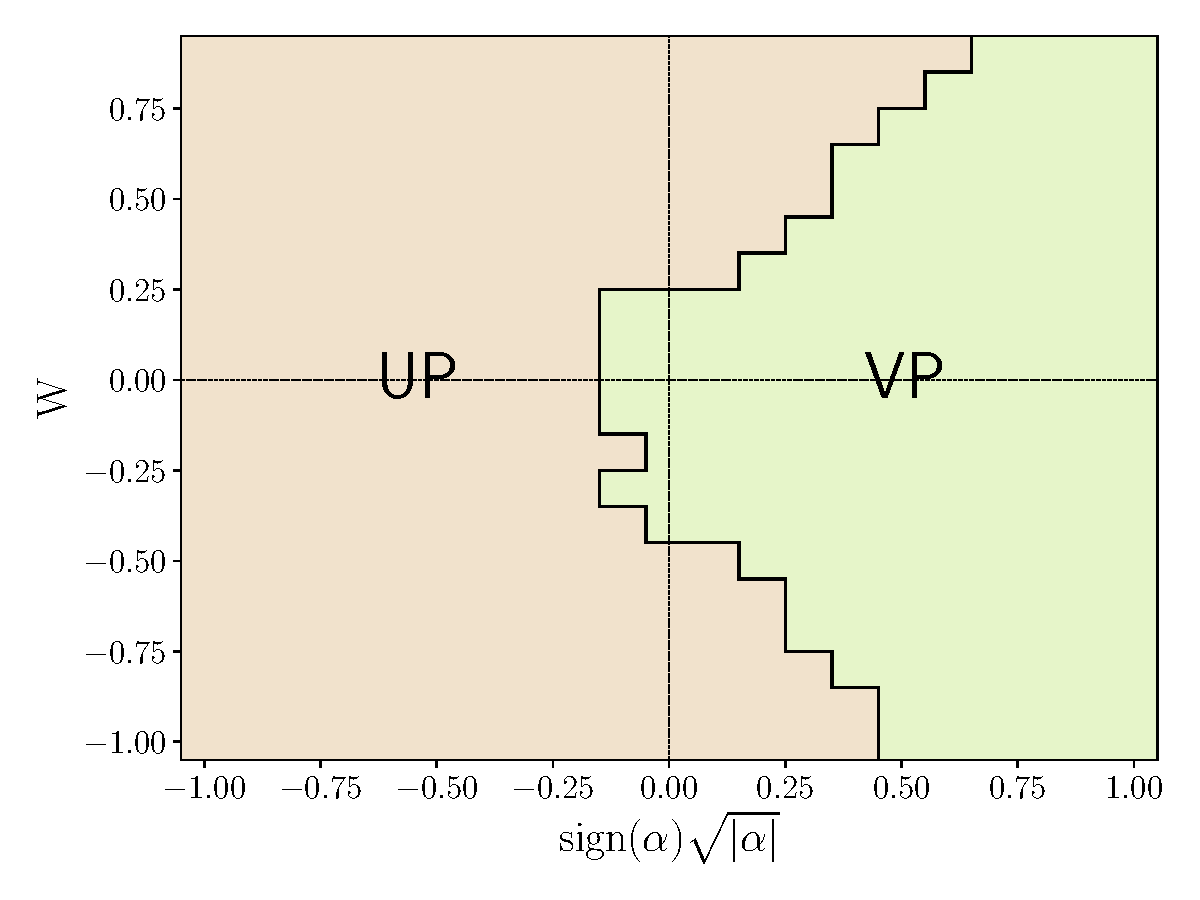
\includegraphics[width=1.0\textwidth]{plots/fourth_fourth_q0_phase_diagram.pdf}
        \subcaption{$U(\mathbf{q}=0) = 0$}\label{fig:fourth_fourth_q0_phase_diagram}
    \end{subfigure}
    \caption{Phase diagrams of the $\nu = \frac{1}{2}$ filling. VP:\@ gapless valley-polarized state. UP:\@ general unpolarized state. See Fig.~\ref{fig:summary} for a schematic identification of the VP/UP regions.}\label{fig:fourth_fourth_phases}
\end{figure}



Figure~\ref{fig:fourth_fourth_phases} shows the resulting phase diagram. With $U(\mathbf{q}=0)\neq 0$, two gapless phases are present: a VP phase at low $\alpha$ or low $|W|$, and a non-polarized phase otherwise. Following the same reasoning as for $\nu=1$, the $\alpha=1$, $W=0$ limit is expected to host a $\ket{\text{CFL}} \otimes \overline{\ket{\text{CFL}}}$ state at $\nu=\tfrac{1}{4} + \tfrac{1}{4}$, while the gapless phase at $\alpha=1$ and high $|W|$ is expected to be $\ket{\text{FL}} \otimes \overline{\ket{\text{FL}}}$; the intermediate parameter regime is harder to characterize unambiguously.

Unlike at the other fillings, the VP state here is similar in nature to the unpolarized state. At $W=0$, the fully valley-polarized system is a $\text{CFL}_{\text{pol.}}$ for all relevant $\alpha$, since with only one valley occupied the inter-valley coupling plays no role; a Stoner-like transition from the valley-polarized to the unpolarized state is again found at large $|W|$. Once again, the phase diagram is approximately symmetric around the $W=0$ axis.

For the $U(\mathbf{q}=0) = 0$ (Figure~\ref{fig:fourth_fourth_q0_phase_diagram}) the same phases are again detected but with the unpolarized region at low $\alpha$ instead of large $\alpha$. The same Stoner-like transition is found at high $|W|$.

\subsection{\texorpdfstring{Momentum-occupation function}{Momentum-occupation function}}
\begin{figure}[htbp]
    \centering
    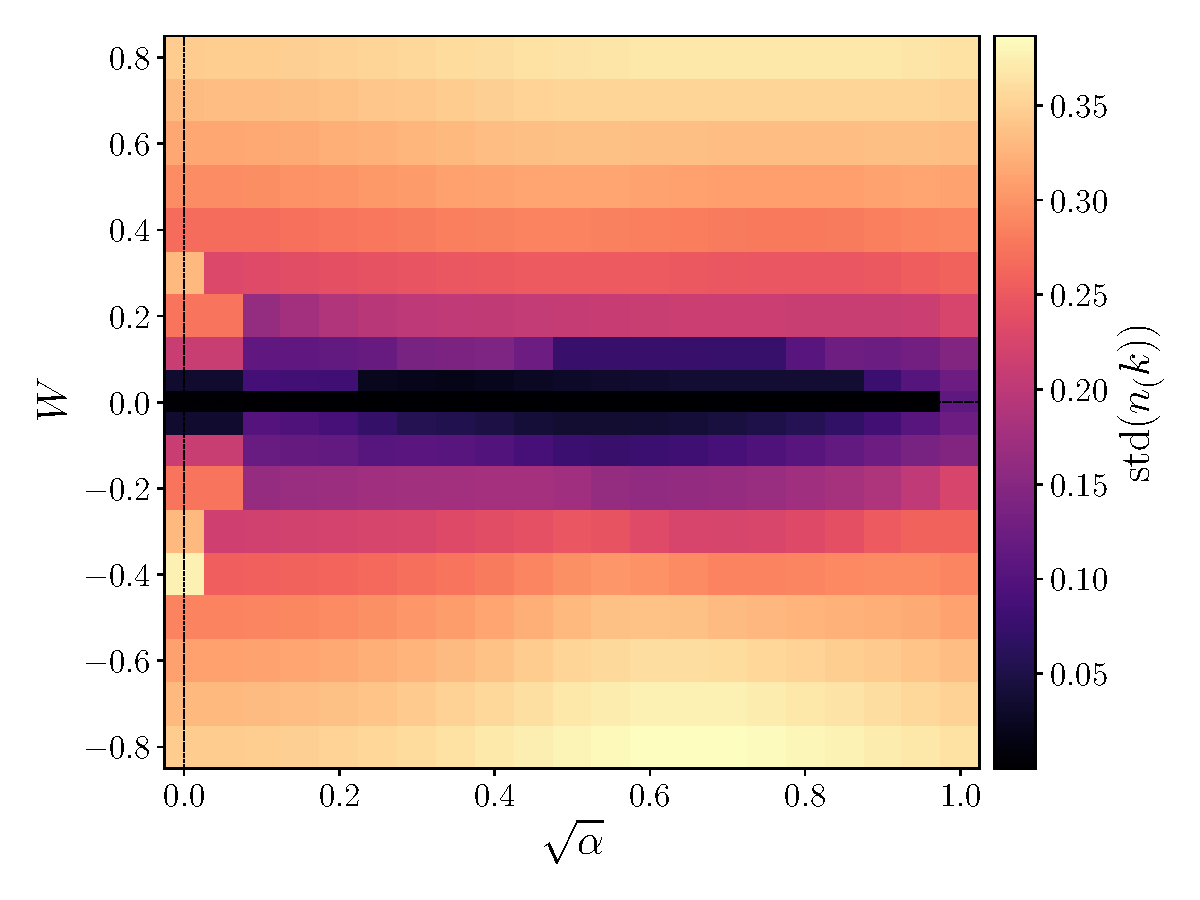
\includegraphics[width=0.5\textwidth]{plots/density_fourth_fourth_std_mesh.pdf}
    \caption{Standard deviation of $n(\mathbf{k})$ over the Brillouin zone as a function of $\alpha$ and $W$, at $\nu=\frac{1}{2}$.}\label{fig:fourth_fourth_density}
\end{figure}

As a further diagnostic for the phases in $U(\mathbf{q} = 0) \neq 0$ case, Fig.~\ref{fig:fourth_fourth_density} shows the standard deviation of $n(\mathbf{k})$ over the Brillouin zone: the occupation is flat at low $|W|$ and develops a clear Fermi surface at high $|W|$. Even though the valley-polarized region is gapless throughout, a clear distinction remains within it between the flat occupation characteristic of a CFL at low $|W|$ and the peaked Fermi surface of an FL at intermediate $|W|$. While not studied in further detail here, a phase transition analogous to the one found at $\nu=1$ is suspected between these states as well.




    \chapter{Results --- first excited Landau level}\label{ch:results_1LL}
    Extending the model to the $n=1$ Landau level modifies the interaction profile: the interaction is effectively multiplied by Laguerre polynomials. While the phase diagram is still expected to partition broadly into valley-polarized and valley-unpolarized regimes, following a similar exchange-driven mechanism, the specific ground-state competition across $(\alpha, W)$ changes.

\section{Anticipated phases}
Across the parameter space, we anticipate the following phase competition:
\begin{itemize}
    \item \textbf{Valley-polarized IQH state (low $W$, small $\alpha$)}: At small inter-valley coupling and low bandwidth, similarly to the LLL case, complete valley polarization is suspected ($\nu = 1 + 0$). Analogously, integer filling in a single valley stabilizes an integer quantum Hall (IQH) state.
    \item \textbf{Paired non-Abelian state ($\alpha = 1$, $W = 0$)}: In the decoupled limit each valley independently hosts a half-filled $n=1$ Landau level ($\nu = \tfrac{1}{2} + \tfrac{1}{2}$). Instead of a composite Fermi liquid, the fermions become unstable to pairing, creating a non-Abelian FTI consisting of two Moore--Read states, $\ket{\mathrm{MR}} \otimes \ket{\overline{\mathrm{MR}}}$ (or $\ket{\mathrm{MR}} \otimes \ket{\mathrm{MR}}$) --- found theoretically in a similar model by Abouelkomsan and Fu~\cite{abouelkomsan2025non}.
    \item \textbf{Depolarization to Fermi liquid (large $W$)}: As the bandwidth $W$ increases, kinetic energy overcomes two-body interactions, eventually forcing a transition to a gapless, unpolarized Fermi liquid (FL).
\end{itemize}

\section{Results for \texorpdfstring{$\nu = 1$}{nu=1} of 1LL (\texorpdfstring{$\nu = 3$}{nu=3} overall)}

Since the Moore--Read state is known to be influenced by the anisotropy of the real-space cluster on which it is defined, tilted boundary conditions were used to stabilize it. To detect the characteristic dependence of the ground-state degeneracy on the fermion-number parity, systems with $N_\phi = 12$ and $N_\phi = 10$ per valley were studied at half filling ($N_e = 12$ and $N_e = 10$, respectively).

\begin{figure}[htbp]
    \centering
    \begin{subfigure}[b]{0.48\textwidth}
        \centering
        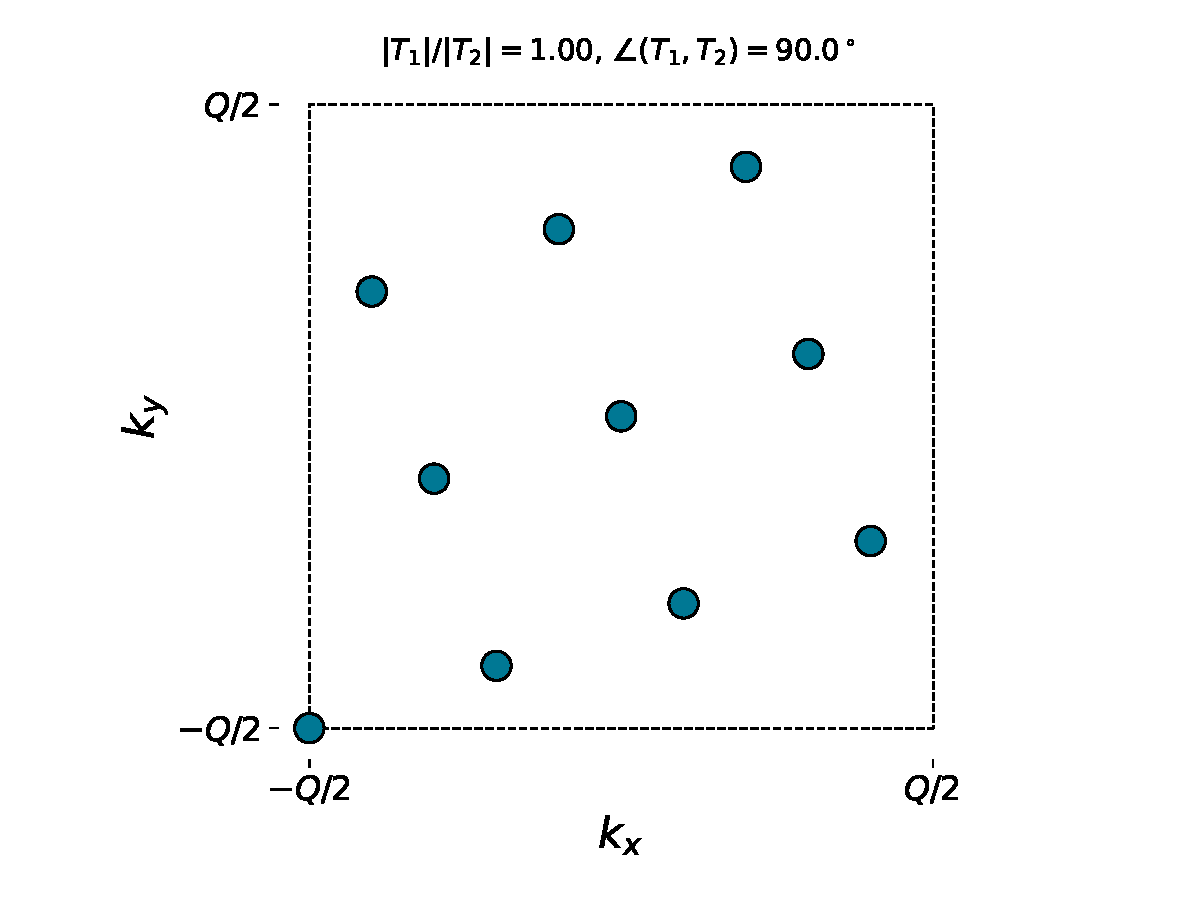
\includegraphics[width=\linewidth]{plots/bz_sampling_tilted_10_ratio=1.000_90.0deg.pdf}
        \caption{$N_\phi = 10$}\label{fig:bz_sampling_10}
    \end{subfigure}
    \begin{subfigure}[b]{0.48\textwidth}
        \centering
        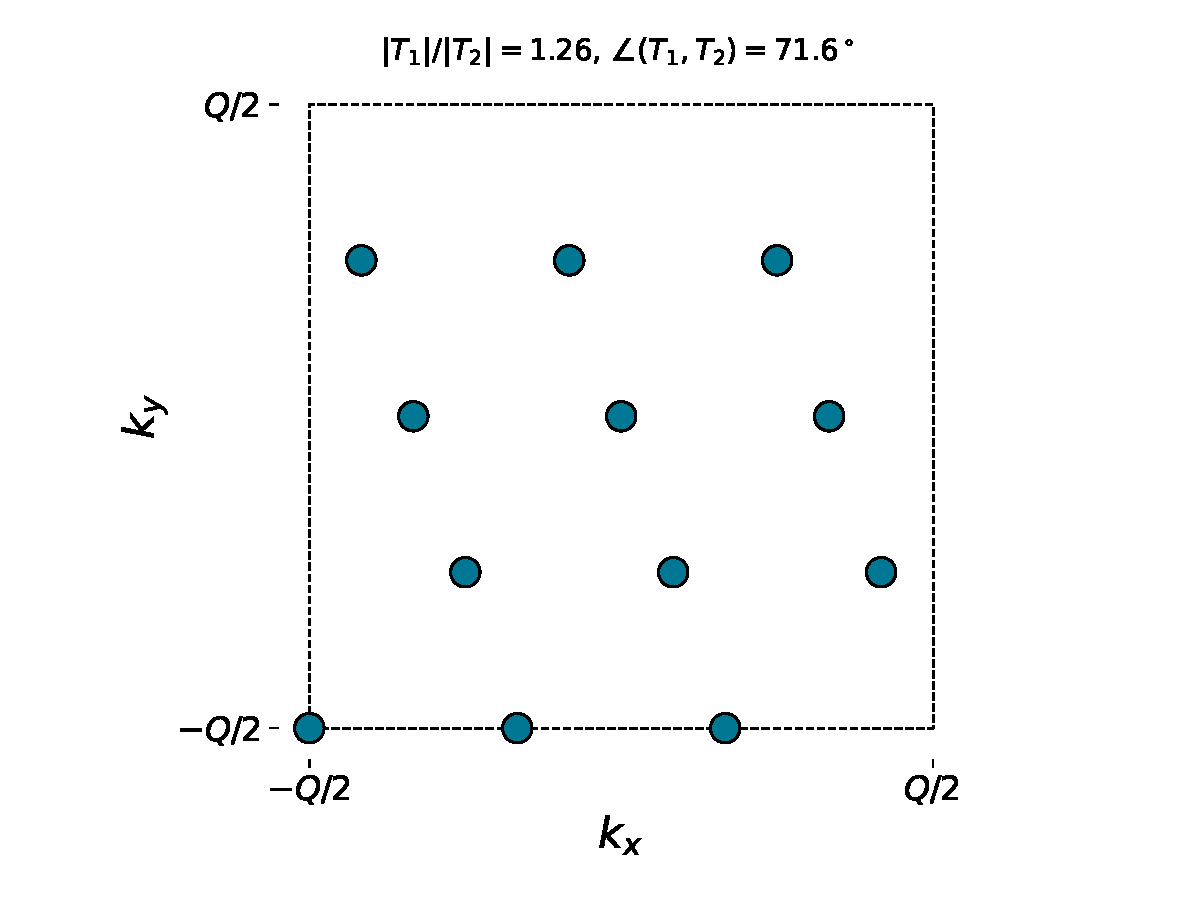
\includegraphics[width=\linewidth]{plots/bz_sampling_tilted_12_ratio=1.265_71.6deg.pdf}
        \caption{$N_\phi = 12$}\label{fig:bz_sampling_12}
    \end{subfigure}
    \caption{BZ sampling for the two system sizes used in the $n=1$ LL calculations, and the properties of the corresponding real-space cluster vectors $T_1$, $T_2$.}
    \label{fig:bz_sampling}
\end{figure}

The tilted lattices used here are shown in Fig.~\ref{fig:bz_sampling}.

\begin{figure}[htbp]
    \centering
    \begin{subfigure}[b]{0.45\textwidth}
        \centering
        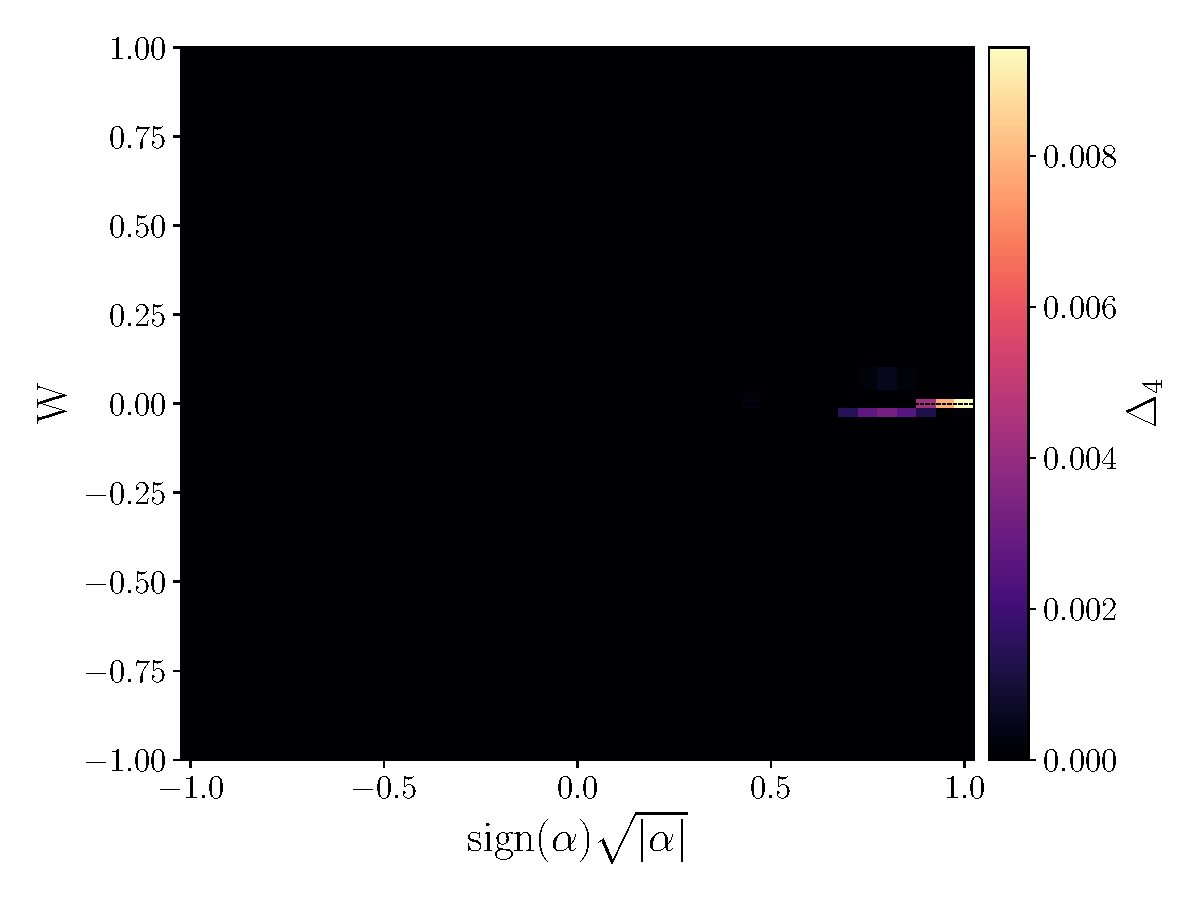
\includegraphics[width=1.0\textwidth]{plots/non_abelian_N10_gap_n4.pdf}
        \subcaption{$\Delta_4$ gap for $N_\phi = 10$ system.}
    \end{subfigure}
    \begin{subfigure}[b]{0.45\textwidth}
        \centering
        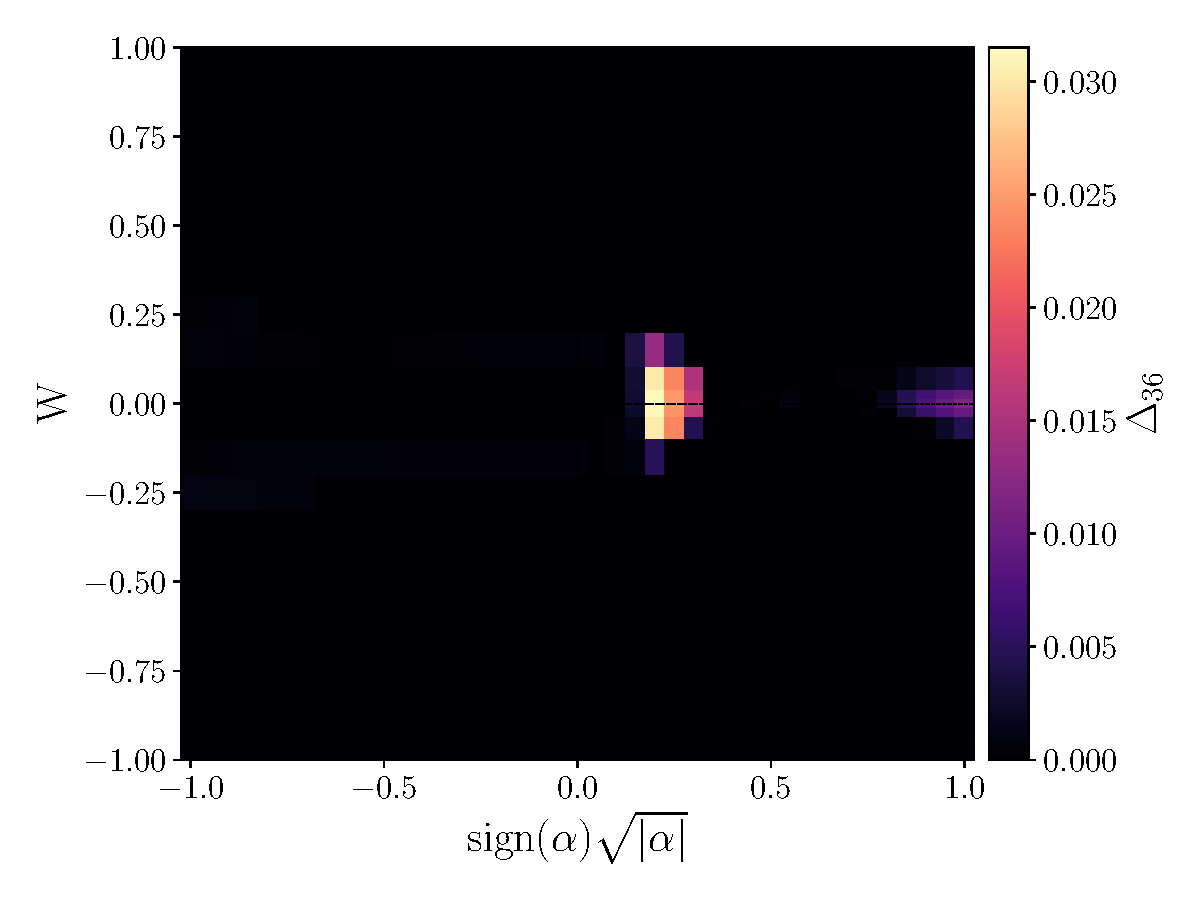
\includegraphics[width=1.0\textwidth]{plots/non_abelian_N12_gap_n36.pdf}
        \subcaption{$\Delta_{36}$ gap for $N_\phi = 12$ system.}\label{fig:non_abelian_gaps_12}
    \end{subfigure}
    \begin{subfigure}[b]{0.45\textwidth}
        \centering
        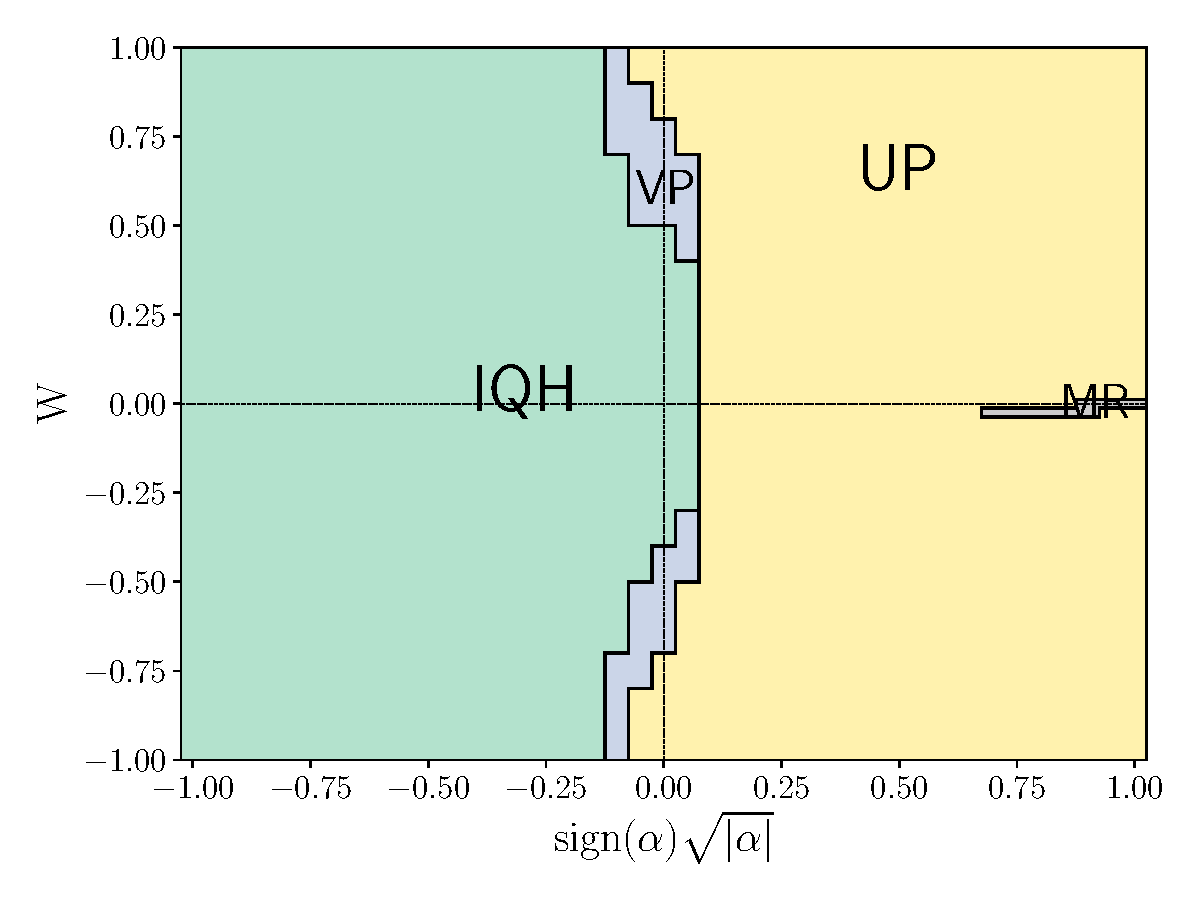
\includegraphics[width=1.0\textwidth]{plots/non_abelian_N10_phase_diagram.pdf}
        \subcaption{Phase diagram for $N_\phi = 10$ system.}
    \end{subfigure}
    \begin{subfigure}[b]{0.45\textwidth}
        \centering
        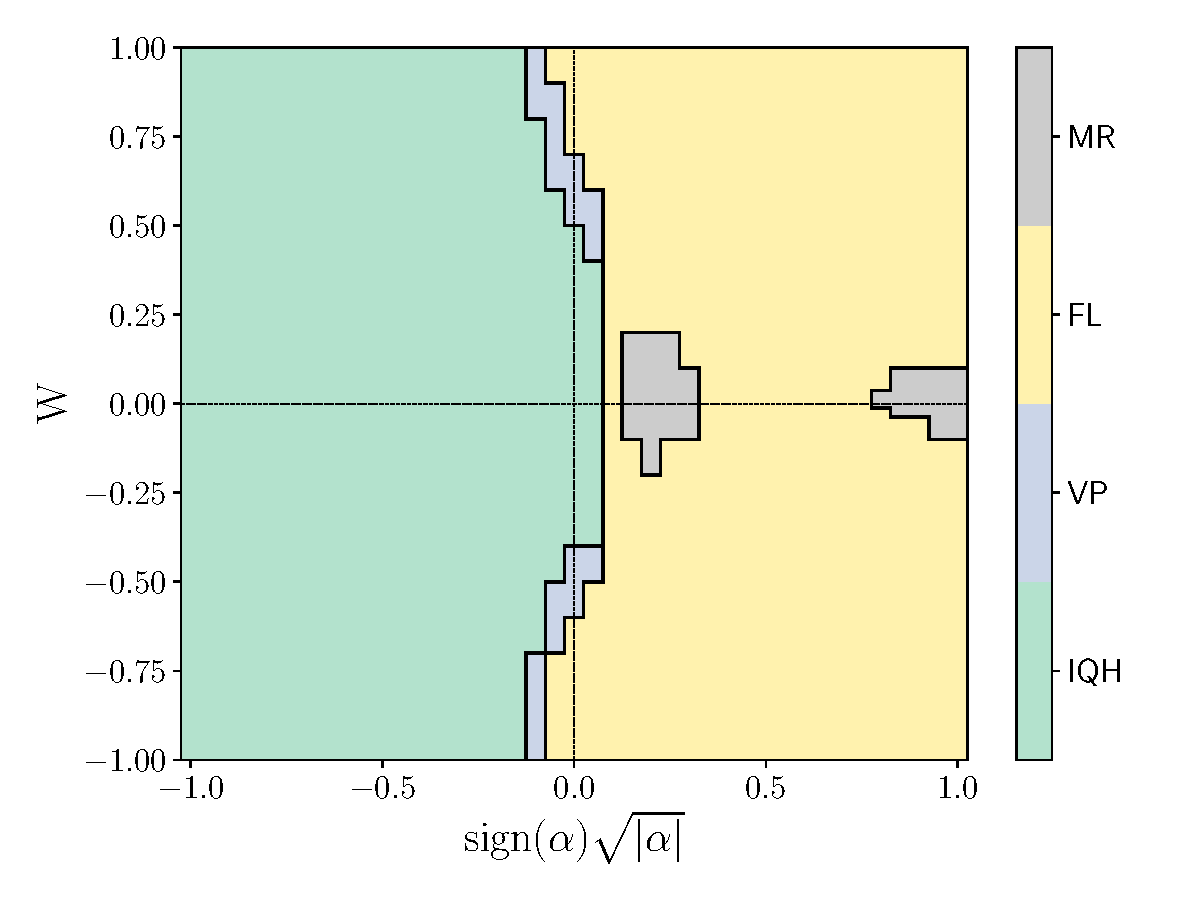
\includegraphics[width=1.0\textwidth]{plots/non_abelian_N12_phase_diagram.pdf}
        \subcaption{Phase diagram for $N_\phi = 12$ system.}
    \end{subfigure}
    \caption{The low-$\alpha$ gapped phase could be just a CDW or something similar --- from a rough look at the flux insertion there is no spectral flow, it seems.}
    \label{fig:non_abelian_gaps}
\end{figure}

Figure~\ref{fig:non_abelian_gaps} shows the $\Delta_4$ and $\Delta_{36}$ gaps for the two system sizes, as well as the schematic phase diagrams. The suspected results are confirmed: at low $\alpha$ and low $W$ the system is in a gapped, valley-polarized phase --- the IQH phase --- and the gap closes at large $W$ as the system transitions to a gapless Fermi liquid, first valley-polarized, then unpolarized. At $\alpha = 1$, $W = 0$, the system is in a gapped, unpolarized phase with 4-fold and 36-fold degeneracy for $N_\phi = 10$ and $N_\phi = 12$ respectively, which is consistent with the expected non-Abelian FTI phase.

\subsection{Problems with the \texorpdfstring{$N_\phi = 12$}{Nphi=12} system}

\begin{figure}[htbp]
    \centering
    \begin{subfigure}[b]{0.48\textwidth}
        \centering
        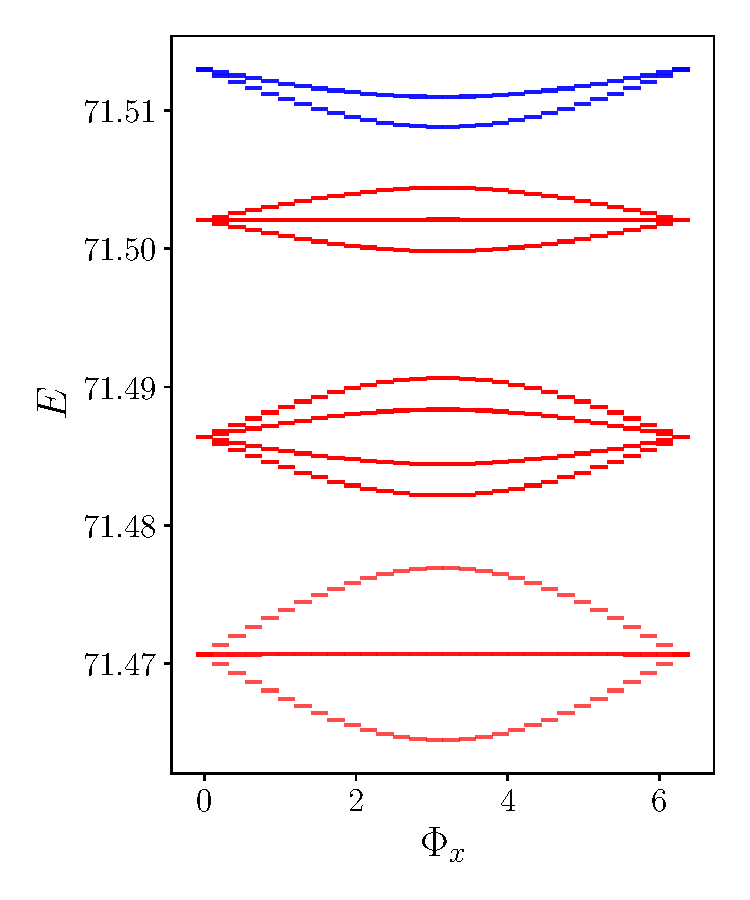
\includegraphics[width=\linewidth]{plots/phase_winding_moore_read_W=0.05_alpha=1.0.pdf}
        \caption{$\alpha = 1.0$}\label{fig:phase_winding_moore_read}
    \end{subfigure}
    \begin{subfigure}[b]{0.48\textwidth}
        \centering
        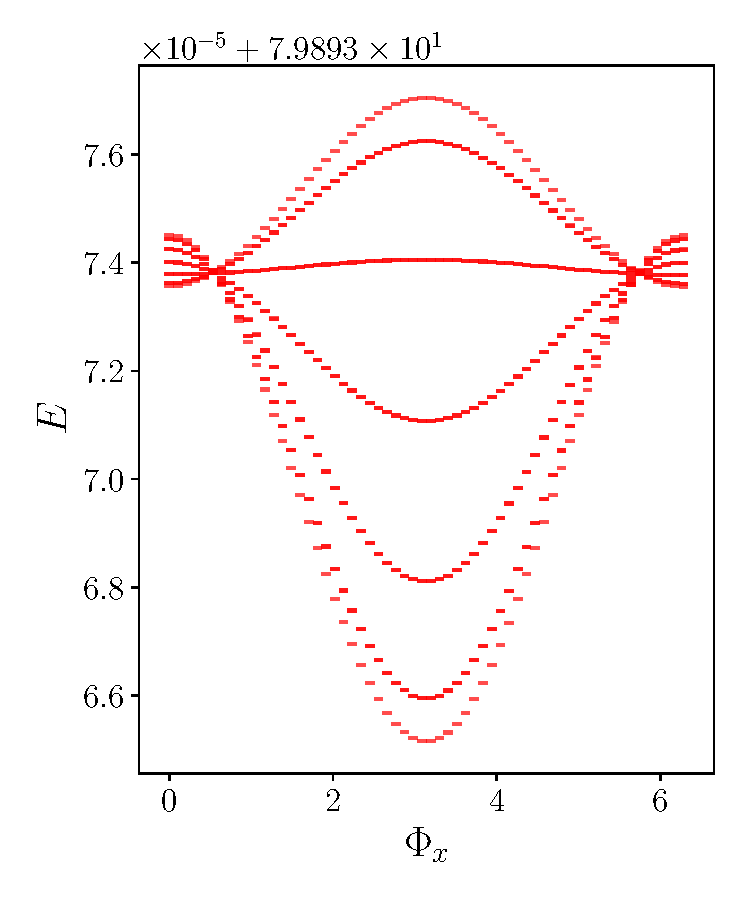
\includegraphics[width=\linewidth]{plots/phase_winding_moore_read_W=0.05_alpha=0.07.pdf}
        \caption{$\alpha = 0.07$}\label{fig:phase_winding_cdw}
    \end{subfigure}
    \caption{Phase winding for $N_\phi = 12$ at $W = 0.05$.}
    \label{fig:phase_winding_1LL}
\end{figure}

Figure~\ref{fig:phase_winding_moore_read} shows a flux-insertion plot for the $N_\phi = 12$ system at $\alpha = 1$, $W = 0.05$. The 36-fold degenerate ground-state manifold is clearly visible, and spectral flow is seen between groups of states in the manifold. However, the gap between the 36-fold degenerate ground-state manifold and the first excited state is in fact smaller than the spread of energies in the ground-state manifold itself. While this is an indication of questionable stability of the phase, it is not a definitive argument against it, as explained below in Sec.~\ref{sec:gap_ratio}.

Second, at the lower end of the unpolarized phase, the size of the $\Delta_{36}$ gap is also quite large (Fig.~\ref{fig:non_abelian_gaps_12}) --- the region is not adiabatically connected to the $\alpha = 1$, $W = 0$ point. Under inspection of the flux insertion (Fig.~\ref{fig:phase_winding_cdw}), it is seen that the spectral flow is not present in this region. The phase is not topological in nature, likely a charge density wave (CDW), and it is not studied further.

\subsection{Discussion of the gap ratio}\label{sec:gap_ratio}

In the literature, due to finite-size effects and dispersion making the ground-state degeneracy only approximate, instead of the direct spectral gap, the ratio of the energy spread $\delta_n$ of the $n$-fold degenerate ground-state manifold to the $\Delta_n$ gap is often considered, with the premise that
\[
    \frac{\delta_n}{\Delta_n} = 0
\]
indicates a perfectly degenerate ground state~\cite{kwan2024could}. A condition of
\[
    \frac{\delta_n}{\Delta_n} < 1
\]
is often used to indicate a good candidate for a topological phase.

Here, I argue that this condition might be too strong when considering a topological insulator made of two decoupled copies of a Chern insulator, $\ket{\mathrm{FTI}} = \ket{\mathrm{FCI}}_- \otimes \ket{\overline{\mathrm{FCI}}}_+$.

Let $E_L$ and $E_H$ be the energies of the lowest and highest states in the $n$-fold degenerate ground-state manifold of the single $\ket{\mathrm{FCI}}_\pm$, and let $E_E$ be the energy of the first excited state. Then $\Delta_n^{\mathrm{FCI\pm}} = E_E^{\mathrm{FCI}} - E_H^{\mathrm{FCI}}$ and $\delta_n^{\mathrm{FCI\pm}} = E_H^{\mathrm{FCI}} - E_L^{\mathrm{FCI}}$, and the ratio of interest is
\[
    \frac{\delta_n^{\mathrm{FCI\pm}}}{\Delta_n^{\mathrm{FCI\pm}}} = \frac{E_H^{\mathrm{FCI}} - E_L^{\mathrm{FCI}}}{E_E^{\mathrm{FCI}} - E_H^{\mathrm{FCI}}}.
\]
The condition imposed for a good topological state is
\[
    \frac{E_H^{\mathrm{FCI}} - E_L^{\mathrm{FCI}}}{E_E^{\mathrm{FCI}} - E_H^{\mathrm{FCI}}} < 1
    \implies
    E_E^{\mathrm{FCI}} - E_H^{\mathrm{FCI}} > E_H^{\mathrm{FCI}} - E_L^{\mathrm{FCI}}
    \implies
    E_E^{\mathrm{FCI}} + E_L^{\mathrm{FCI}} > 2 E_H^{\mathrm{FCI}}.
\]

However, the energies of the $\ket{\mathrm{FTI}}$ are simply the sum of energies of the underlying $\ket{\mathrm{FCI}}_\pm$ states. Thus,
\[
    E_L^{\mathrm{FTI}} = E_L^{\mathrm{FCI}} + E_L^{\mathrm{FCI}}, \qquad
    E_H^{\mathrm{FTI}} = E_H^{\mathrm{FCI}} + E_H^{\mathrm{FCI}}, \qquad
    E_E^{\mathrm{FTI}} = E_L^{\mathrm{FCI}} + E_E^{\mathrm{FCI}},
\]
and
\[
    \Delta_{n^2}^{\mathrm{FTI}} = E_E^{\mathrm{FTI}} - E_H^{\mathrm{FTI}} = E_L^{\mathrm{FCI}} + E_E^{\mathrm{FCI}} - 2 E_H^{\mathrm{FCI}},
\]
which, with the condition imposed above for the FCI, gives simply
\[
    \Delta_{n^2}^{\mathrm{FTI}} > 0.
\]

Thus, the condition for existence of a non-zero gap in the FTI constructed from two decoupled FCI states is equivalent to the condition for a good topological state in the underlying FCI. The condition $\delta_n^{\mathrm{FTI}}/\Delta_n^{\mathrm{FTI}} < 1$ is much stronger than that.

\subsection{Stabilizing the FTI phase --- screening dependence}

Since the non-Abelian FTI phase has a large spread of energies in the ground-state manifold, its stability is tested against the screening parameters $d_{\mathrm{SC}}$ and $l_{\mathrm{RK}}$. For simplicity, the decoupled limit $\alpha = 1$, $W = 0$ is considered, which means each valley can be treated independently --- thus only a single-valley model is considered, where instead of 36-fold degeneracy, a 6-fold degeneracy is expected.

\begin{figure}[htbp]
    \centering
    \begin{subfigure}[b]{0.48\textwidth}
        \centering
        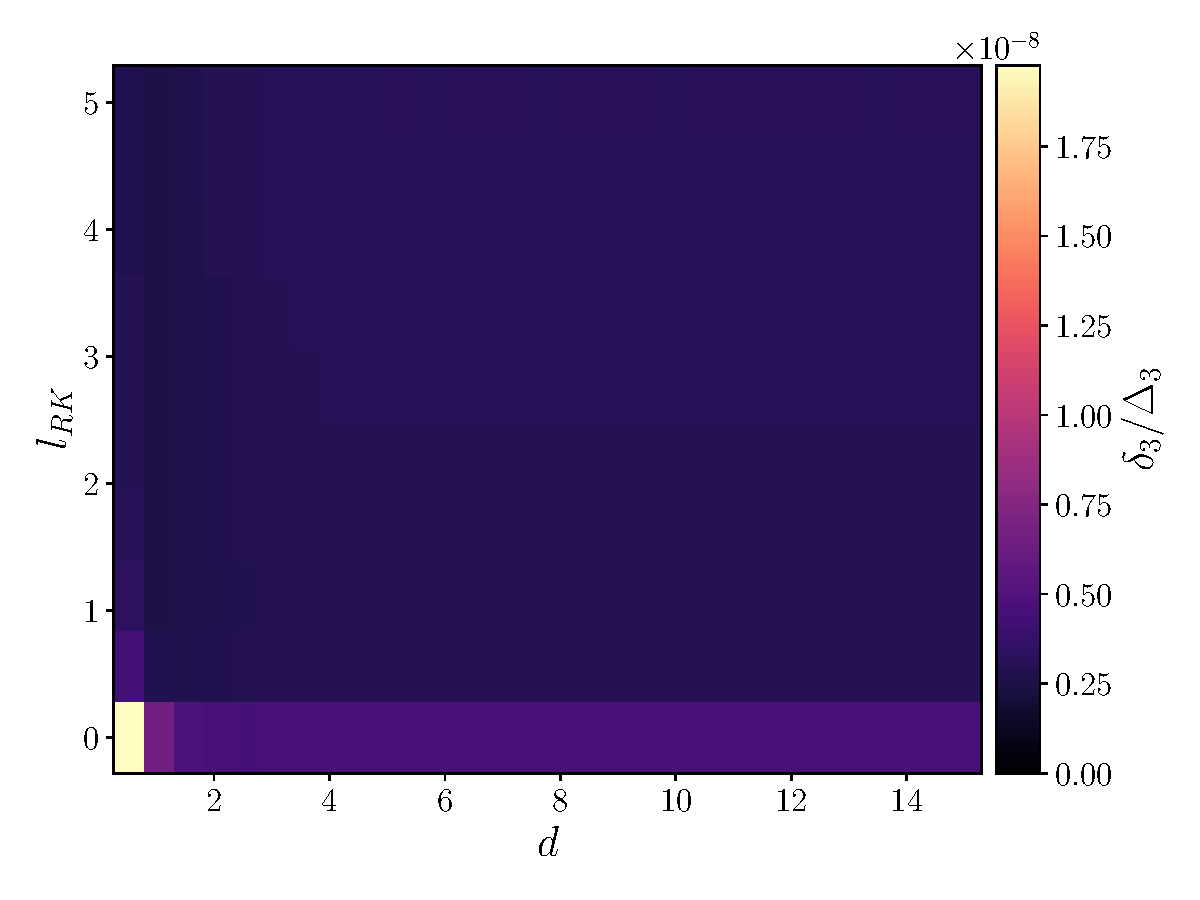
\includegraphics[width=\linewidth]{plots/LLL_stability_n3.pdf}
        \caption{Lowest Landau level}\label{fig:LLL_stability_n3}
    \end{subfigure}
    \begin{subfigure}[b]{0.48\textwidth}
        \centering
        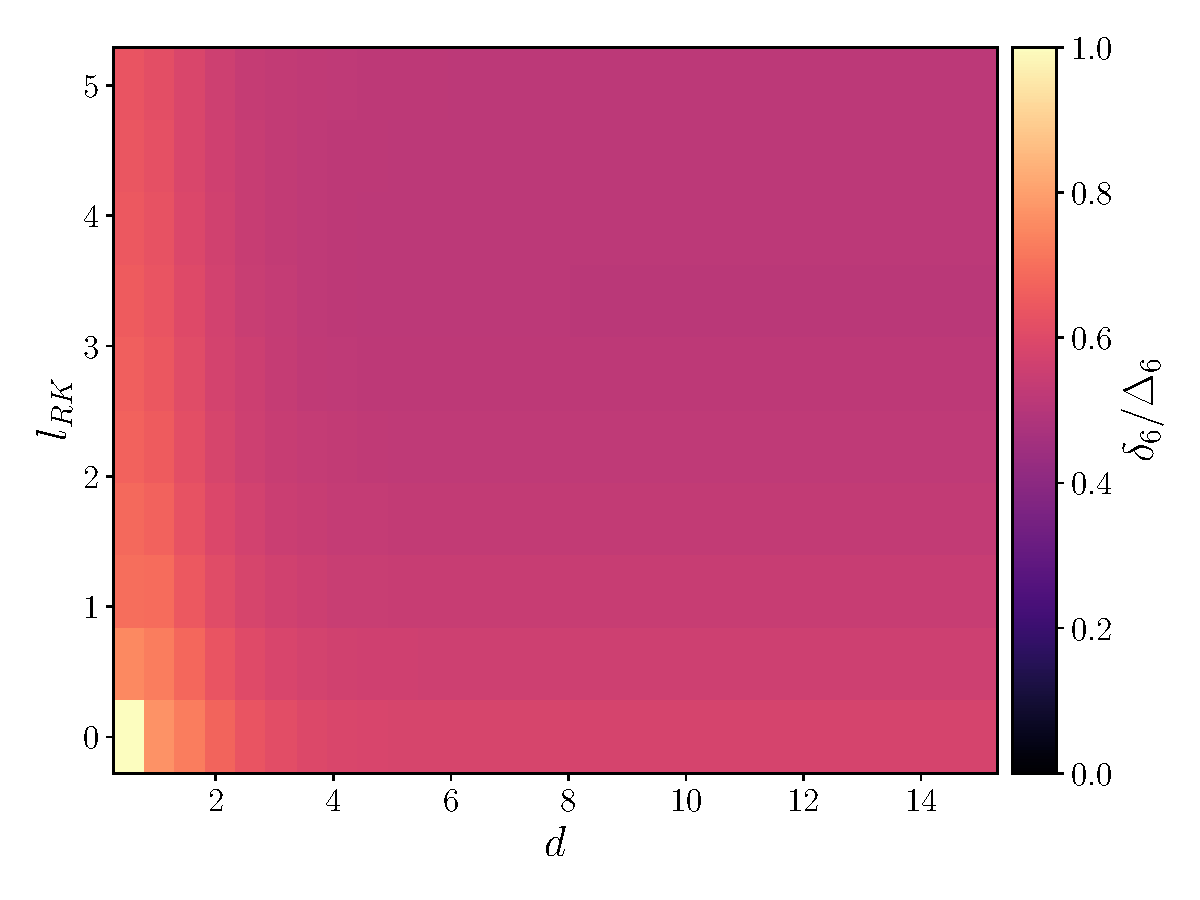
\includegraphics[width=\linewidth]{plots/1LL_stability_n6.pdf}
        \caption{$n=1$ Landau level}\label{fig:1LL_stability_n6}
    \end{subfigure}
    \caption{$\delta_6/\Delta_6$ ratio in one decoupled $\ket{\mathrm{FCI}}$ state corresponding to $W=0$ and $\alpha=1$. Value near zero means good stability.}
    \label{fig:stability_phases}
\end{figure}

In Fig.~\ref{fig:1LL_stability_n6}, the dependence of the $\delta_6/\Delta_6$ ratio on the screening parameters is shown. It is seen that the ratio decreases monotonically with increasing $d_{\mathrm{SC}}$ and $l_{\mathrm{RK}}$. However, comparing with a similar plot for the single-valley $\nu=1/3$ FCI state (Fig.~\ref{fig:LLL_stability_n3}), the ratio is much larger for the $\nu=1/2$ Moore--Read state. While for the lowest Landau level FCI it is consistently close to 0, for the $n=1$ Landau level it does not fall below the $0.5$ threshold. This indicates that the screening of the Coulomb interaction is not sufficient to stabilize the non-Abelian FTI phase.

However, it is important to note that the stability of the FTI phase shown here at the $\alpha=1$ point does not correspond to the stability of the FTI phase in the full $(\alpha, W)$ phase diagram. In Figure~\ref{fig:third_third_screening_alpha_vs_lRK_phase_diagram_b} a maximum of inter--valley coupling stability was seen at $l_{\mathrm{RK}} \neq 0$, while here, the $\delta/\Delta$ ratio decreases monotonically with increasing $l_{\mathrm{RK}}$. This furhter shows the importance of considering the inter-valley interaction.


    \chapter{Conclusions and outlook}\label{ch:conclusions}
    
\section{Limitations}

Several limitations of the present work should be kept in mind when interpreting
the results of Chapter~\ref{ch:results} and Chapter~\ref{ch:results_1LL}.

\paragraph{Finite-size effects.} All results are obtained by exact diagonalization
on a single system size (a $3 \times 4$ torus for the phase diagrams, with a
separate tilted geometry for the momentum-occupation calculations of \S\ref{sec:third_third_intermediate_phases}
onward). As discussed in \S\ref{sec:recognition}, a rigorous identification of topological order
requires finite-size scaling --- confirming that the many-body gap remains open and
the ground-state degeneracy persists as the system size increases --- which was not
performed here due to computational cost. The phase boundaries reported in
Chapter~\ref{ch:results} and Chapter~\ref{ch:results_1LL} should therefore be understood as consistent with, rather than a
definitive proof of, the identified phases; in particular, the precise location of
phase boundaries (e.g.\ $\alpha_c$, $W_c$) is expected to shift with system size,
even where the qualitative phase structure is robust.

\paragraph{Momentum grid choice.} Related to the above, the untilted rectangular
momentum grid used by default (\S\ref{sec:tilted_bc}) is known to bias the competition between
topological and charge-density-wave-like states relative to more isotropic tilted
grids~\cite{lauchli2013hierarchy}. While this choice was made for simplicity and
consistency across the phase diagrams, it means the reported phase boundaries may
not be fully representative of the thermodynamic-limit behavior.

\paragraph{Treatment of the $q=0$ interaction component.} As noted in \S\ref{sec:interactions}, the
``background-subtracted'' variant of the interaction removes the full
$q \to 0$ component of $\tilde{U}_{\tau\tau'}(q)$ for all $\tau, \tau'$, rather than
only the part that couples to the total charge density. This is a simplification of
the standard neutralizing-background convention, and the $\alpha$-dependence of the
discarded component is in principle physical. The qualitative difference between the
two phase diagrams shown throughout Chapter~4 (with and without this subtraction)
suggests this choice is not negligible, and a more careful treatment is left for
future work.

\paragraph{Model scope.} The model of Chapter~2 captures the two-valley
Landau-level physics of Moir\'e TMDs at a single magic angle, projected onto a
single (Landau-level-like) band per valley, and neglects Landau-level mixing. Real Moir\'e TMD flat bands deviate from
ideal Landau levels in ways not captured by this construction (e.g.\ non-uniform
Berry curvature, deviations of the form factor from the ideal Gaussian form), and a
quantitative comparison to specific materials (e.g.\ MoTe$_2$ at
$\theta \approx 1.89^\circ$) would require using the actual continuum-model form
factors rather than the idealized Landau-level ones used here.

\paragraph{Unresolved intermediate phases.} Several regions of the phase diagrams
-- most notably the narrow 3-fold-degenerate region near the FTI--gapless boundary
at $\nu = 2/3$ (\S4.3.3), the candidate IVC regions inferred from flat momentum
occupation at $\nu = 2/3$ and $\nu = 1$ (\S4.3.3, \S4.4), and the
$|\mathrm{CFL}\rangle \otimes |\mathrm{CFL}\rangle$--$|\mathrm{FL}\rangle \otimes
|\mathrm{FL}\rangle$ transition at $\nu = 1$ (\S4.4) -- were identified only
indirectly, through the degeneracy/spectral-flow/occupation diagnostics of \S3.4,
rather than through direct comparison with model wavefunctions. A more conclusive
identification of these states would require computing their overlap with
candidate trial wavefunctions (e.g.\ the Halperin $(1,1,2)$ state), which was
beyond the scope of this thesis.


% ------------------------------------------------------------
% 4. CONCLUSIONS
% Final chapter (or final section of Ch. 5, as preferred).
% ------------------------------------------------------------

\section{Conclusions}

This thesis studied a two-valley Landau-level model designed to capture the
essential physics of correlated and topological phases in Moir\'e transition metal
dichalcogenides, using exact diagonalization on finite tori. At filling
$\nu = 2/3$, we found clear numerical evidence --- via ground-state degeneracy and
spectral flow --- for a valley-polarized fractional quantum Hall
state at small inter-valley coupling $\alpha$ and small bandwidth $W$, and for a
valley-unpolarized fractional topological insulator built from two time-reversed
Laughlin copies at large $\alpha$, consistent with theoretical expectations. Both
phases were shown to survive a finite bandwidth and finite screening length, with
stability boundaries that depend systematically on $d_{\mathrm{SC}}$ and
$l_{\mathrm{RK}}$. At $\nu = 1$ and $\nu = 1/2$, we recovered the expected
valley-polarized integer quantum Hall state and decoupled composite-Fermi-liquid
pairs, respectively, together with signatures of an intervening
inter-valley-coherent regime at large $|W|$.

An analytic Hartree--Fock treatment of the valley-depolarization transition,
developed for both the $\alpha$-driven and $W$-driven cases, reproduced the correct
qualitative trends of the numerical phase diagrams -- including the direction of
the phase boundaries with $d_{\mathrm{SC}}$ and $l_{\mathrm{RK}}$ -- while
systematically overestimating the critical $\alpha_c$ and $W_c$ by up to an order
of magnitude, a discrepancy attributed largely to the circular-Fermi-surface
approximation used in the mean-field derivation.

Taken together, these results support the picture of Moir\'e TMDs as a
magnetic-field-free platform for realizing both fractional Chern insulator and
fractional topological insulator physics, and provide a systematic account of how
this physics competes with bandwidth, inter-valley coupling, and dielectric
screening within a single, tunable model. The main open questions raised by this
work --- the precise nature of the intermediate phases identified only indirectly in
\S4.3--4.4, the role of finite-size effects, and the extension to non-Abelian
Moore--Read-like states in the first excited Landau level --- are left for future work.
    \newpage

    %\nocite{*}
    \printbibliography

    \newpage
    \appendix
    

\chapter{Explanations and questions to Glenn}

In the draft, mainly in the results section, I have provided some theories and explanations of the seen phases and transitions which we haven't discussed yet. Namely, the IVC phase --- and its possible transition to the FL phase, as well as the 3-fold degenerate gapped phase in unpolarized region of $\nu = 2/3$ filling. I provided some references to the literature which I used to get these ideas, but I am not at all sure if it is correct so please treat it more as a question than a statement. Does this make sense, or maybe there is something I am missing which busts these explanations?
\\
\\

I found a bug in the calculation of the inter valley coherence --- instead of IVC\^2 order paramter I just calculated the inter valley density-density correlation function / structure factor... Unfortunately this also means that the DiagHam density code does not even produce the correct matrix terms so I cannot calculate the IVC order parameter at all. 
What I did calculate using this, are the inter and intra-valley static structure factors, however, I was not able to infer anything useful from them yet --- I did not add it to the thesis.
\\
\\
I made quite a big mistake calculating the $U(q=0)=0$ phase diagrams I believe --- what i should cancel is just the total-density part of the interaction, meanwhile I just zeroed out the WHOLE $U(q=0)$ term. For now I just left in these phase diagrams and commented shortly on the interaction used, but probably recalculating them with correct interaction would be a good idea.


I also have a bit  more results:
\begin{itemize}
    \item I have the comparison of Haldane pseudopotentials between different screenings and different Landau levels, which I can add (along with explanation of the pseudopotentials themselves in the introduction)
    \item I already have additional plots ready --- different spectral gaps at all of the fillings, and also the \textit{relative} gaps (gap\_inside\_GS\_manifold / gap\_to\_first\_excited\_state). I was thinking about adding them but I don't see if they bring much added value compared to what I already have --- the relative gap in abelian topological phases is very close to zero (as it should be) and then it grows quite quickly to high values near the phase boundaries.
    \item I could also add the phase transitions $\alpha=0$, increasing $W$ and $W=0$, increasing $\alpha$ to compare them with the ones in the textured exciton insulators paper
    \item I am quite close to calculating the Chern number numerically
    \item I have some earlier results for systems WITHOUT the valley degree of freedom --- just single valley. But again I am not sure if they provide any additional information.
\end{itemize}


\end{document}
